% !TEX TS-program = LuaLaTeX
\documentclass[10pt, oneside, a4paper]{article}

\usepackage[T1]{fontenc}
\usepackage{lmodern}
\usepackage{xcolor}
    \definecolor{gray} {HTML}{363636}
    \definecolor{red}  {HTML}{950009}
    \definecolor{green}{HTML}{0E610A}
    \definecolor{blue} {HTML}{020069}
\usepackage{fontspec}
    \setsansfont{Arial}
\usepackage{amsmath}
\usepackage{titlesec}
    \titleformat*{\section}      {\color{gray}\large\bfseries\sffamily}
    \titleformat*{\subsection}   {\color{gray}\large\bfseries\sffamily}
    \titleformat*{\subsubsection}{\color{gray}\large\bfseries\sffamily}
\usepackage{geometry}
    \geometry{scale={0.75,0.85}}
\usepackage{siunitx}
    \sisetup{locale=FR}
    \sisetup{math-micro=\text{µ},text-micro=µ} % fix
\usepackage{graphicx}
\usepackage{caption}
    \captionsetup{labelfont={bf,sf,color=gray}}
\usepackage{pdfpages}
\usepackage{caption}

\usepackage{mwe} % For dummy images
\usepackage{subcaption}

\usepackage{fancyhdr}
\pagestyle{fancy}
\fancyhead[R]{}
\fancyfoot[L]{Thomas Anizet}
\fancyfoot[C]{}
\fancyfoot[R]{\thepage}

\usepackage{rotating}
\usepackage{tikz}


% Keep lasts
\usepackage[french]{babel}
    \frenchsetup{SmallCapsFigTabCaptions=false}
\usepackage[expansion]{microtype}
\usepackage[luatex, backref]{hyperref}
    \hypersetup{unicode, colorlinks, breaklinks, urlcolor=red,
                bookmarksopen, bookmarksnumbered}

\renewcommand{\UrlFont}{\small}
\renewcommand{\arraystretch}{1.1}
\setlength{\parskip}{2mm}

\begin{document}


%%%%%%%%%%%%%%%%%%%%%%%% Table des matières
\tableofcontents
\newpage

%%%%%%%%%%%%%%%%%%%%%%%% Introduction

\phantomsection
\section*{Introduction}
\addcontentsline{toc}{section}{Introduction}

Candidat "Officier de carrière" à l’\textbf{\textit{École Royale Militaire}} (ERM), je suis actuellement ma formation académique à l’\textbf{\textit{École Centrale des Arts et Métiers}} (ECAM) en option électronique. \\ \\
Durant notre 2ème année de Master, les étudiants doivent réaliser un stage d’immersion en entreprise d’une durée de six semaines. Ce stage consiste, entre autres, à s’insérer dans une entreprise afin d’y découvrir différents aspects tels que l’organisation générale d’une entreprise, son vécu, sa structure interne et ses domaines d'activité. Il a également pour but de se familiariser au travail quotidien de l’ingénieur en participant de façon autonome à diverses activités. \\ \\
Ayant réalisé mon stage de 3ème Bachelier chez \textbf{\textit{AIRBUS DS SLC}} sur le site de Diegem et de Elancourt, il était important pour moi de saisir la chance et l’opportunité de découvrir une nouvelle entreprise renommée à travers le monde. C'est ainsi que je décidai de réaliser mon stage chez \textit{\textbf{THALES} Telecommunications Belgium} sur le site de Tubize. L'objectif principal de ce stage de six semaines fut essentiellement d'introduire et de parcourir l'ensemble des notions théoriques et pratiques sur un sujet peu connu à l'heure actuelle : les \textit{"Side Channel Attacks"} (SCA). En effet, devant réaliser par la suite mon \textit{Travail de Fin d'Étude} (TFE) chez Thales, ce stage devait me permettre d'apprendre et de développer le bagage nécessaire pour la mise en oeuvre de mon sujet de TFE, à savoir : \textit{"Développer une contre-mesure pour les attaques par analyse de la consommation de puissance"}.

\newpage

%%%%%%%%%%%%%%%%%%%%%%%% Partie 1 - Environnement de stage %%%%%%%%%%
\section{Environnement de stage}
Cette section a pour objectif de décrire l'entreprise à différents points de vue. Tout d'abord, une description de l'entreprise d'un point de vue historique est abordée. Ensuite, sont détaillés succinctement la structure de l'entreprise, son organisation ainsi que ses domaines d'activités.

\subsection{Historique}
C'est donc chez \textbf{\textit{Thales}} \textit{Telecommunication Belgium} que je me suis rendu pour réaliser mon stage d'immersion en entreprise. Thales est une société anonyme (\textit{S.A.}) d'origine Française. Elle est spécialisée dans cinq domaines clés, à savoir : l'aéronautique, l'espace, la défense, la sécurité et le transport terrestre. Née d'une fusion entre plusieurs entreprises, Thales hérite ainsi d’un passé prestigieux qui remonte à plus d’un siècle. La figure \ref{fig:temps} ci-dessous retrace les dates-clés qui ont permis à Thales de se développer progressivement mais sûrement. \\

\begin{figure}[htbp]
    \centering
    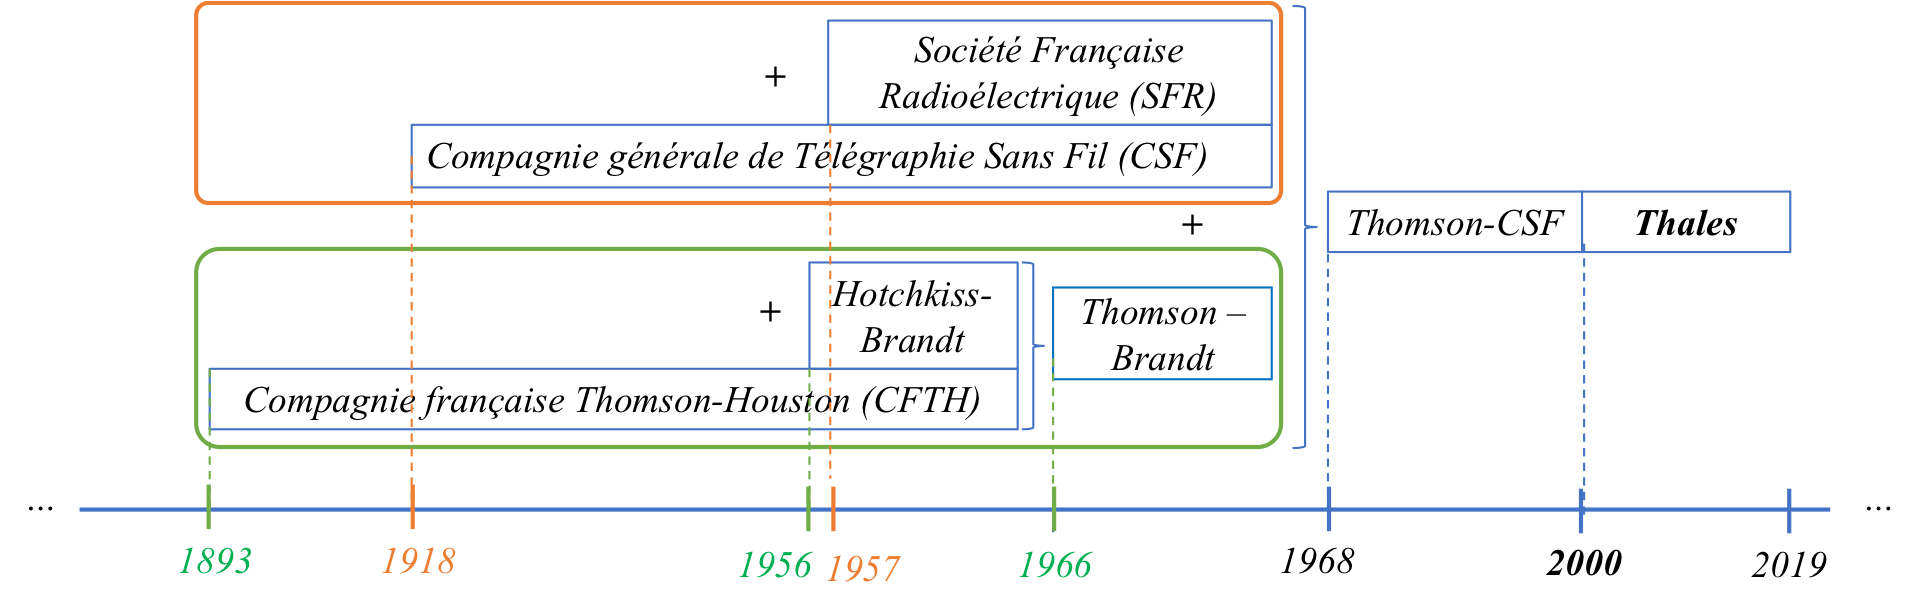
\includegraphics[width=1.\textwidth]{image/temps}
    \caption{Ligne du temps reprenant les dates majeures dans la création de la société \textbf{\textit{Thales}}.}
    \label{fig:temps}
\end{figure}

\hspace{-0.5 cm}Il faut remonter en \underline{\textbf{1893}} pour connaître l'origine de \textit{Thales}. À cette date figure la naissance de la \textbf{\textit{Compagnie Française Thomson-Houston}} (\textit{CFTH}). Cette compagnie avait essentiellement pour but d'exploiter en France les brevets de la société américaine \textit{Thomson-Houston Electric Company}, dans le domaine de la production et du transport de l'électricité. \\ \\
Parallèlement, en \underline{\textbf{1918}} est créé la \textbf{\textit{Compagnie Générale de Télégraphie sans Fil}} (\textit{CSF}) qui deviendra plus tard l'un des pionniers des transmissions hertziennes. En \underline{\textbf{1957}}, \textit{CSF} absorbe la \textbf{\textit{Société Française Radioélectrique}} (\textit{SFR}). Toutes deux tiennent un rôle primordial dans le développement de la radiodiffusion, des radiocommunications sur ondes courtes, de l'électro-acoustique ainsi que du radar et de la télévision. \\ \\
En \underline{\textbf{1966}}, la \textbf{\textit{Compagnie Thomson-Houston}} est renommée \textbf{\textit{Thomson-Brandt}} en raison de sa fusion avec \textbf{\textit{Hotchkiss-Brandt}} (\textit{créé en 1956}), fabriquant d'appareils électroménagers, de voitures, d'armes et de munitions. \\ \\
Deux années plus tard, c'est-à-dire en \underline{\textbf{1968}}, né \textbf{\textit{Thomson-CSF}}, fusion de \textit{CSF} et des activités d'électronique professionnelle de \textit{Thomson-Brandt}. \textit{Thomson-CSF} se développe dans divers domaines. Citons comme exemples les composants électroniques tels que les semi-conducteurs en silicium, l'imagerie médicale ou encore la commutation téléphonique numérique. Cependant, en \underline{\textbf{1982}}, la société est nationalisée en raison d’une situation financière difficile. Cela s’explique par le fait que le portefeuille d’activités est très diversifié, ce qui rend ses parts de marchés trop faibles pour être rentables. Dans les années qui suivent, l’entreprise se recentre sur les activités d’électronique professionnelle et de la défense. \\ \\
En \underline{\textbf{1998}}, \textbf{\textit{Aérospatial}}, \textbf{\textit{Alcatel}}, \textbf{\textit{Dassault Industries}} et \textbf{\textit{Thomson-CSF}} signent un accord de coopération grâce au gouvernant français. À l’issu de celui-ci, \textit{Thomson-CSF} obtient les activités d’électronique professionnelle et de défense \textit{d’Alcatel} et \textit{Dassault Electronique}. De cette façon, \textit{Thomson-CSF} consolide son périmètre d'activité, ses positions concurrentielles dans la défense et l'électronique industrielle, ainsi que son implantation dans plusieurs pays européens. S'en suivent diverses acquisitions à travers le monde, permettant à la société de se développer d’avantage. Ainsi, en \underline{\textbf{juillet 2000}}, une nouvelle organisation en trois pôles est mise en place. Cette organisation s'articule autour de la \textbf{défense}, \textbf{l'aéronautique}, et \textbf{des technologies de l'information et des services}. Cette même année, en \underline{\textbf{décembre 2000}}, pour marquer le coup, \textbf{\textit{Thomson-CSF}} devient la compagnie privée \textbf{\textit{Thales}}. \\ \\
L’organisation actuelle de \textit{Thales} a été mise en place en \underline{\textbf{2007}}, année où \textit{Thales} acquiert les activités de transport, sécurité et aéronautique \textbf{\textit{d’Alcatel-Lucent}}. Cela a permis au groupe de devenir un des leaders mondiaux dans ses domaines d’études. Aujourd’hui, \textit{Thales} est présent dans 56 pays à travers le monde et compte près de 64 000 employés. En 2016, \textit{Thales} affiche un chiffre d’affaire de 14.9 milliards d’euros et a réinvesti près de 731 millions d’euros en \textit{R\&D}. Cela place l’entreprise comme le 10ème acteur mondial dans le domaine de la défense, qui représente 50\% de ses ventes, l’autre part étant générée par le marché civil. \\


\subsection{Structure/Organisation - Domaines d'activité}

Depuis plus de 50 ans, Thales travaille pour les marchés belges de la défense, du spatial, de la sécurité et des transports. Actuellement, le groupe emploie environ 1000 salariés, répartis sur 7 sites à travers la Belgique : Bruxelles, Charleroi, Tubize, Herstal, Genk, Hasselt et enfin Leuven. Le site de Tubize, sur lequel j'ai effectué mon stage, compte environ 150 employés dont une part importante d’ingénieurs et de techniciens. 

\hspace{-0.5 cm}Le groupe laisse à chacune de ses divisions une certaine autonomie, ce qui permet à \textbf{\textit{Thales Belgium}} de fonctionner avec la flexibilité d’une PME tout en bénéficiant de la solidité conférée par un grand groupe international. Elle possède un large panel de compétences : du hardware (conception et production), du software (développement et maintenance), de la sécurité des systèmes développés, de l’ingénierie système via le cycle IVVQ (Intégration, Validation, Vérification, Qualification). En parallèle, des équipes sont en charge des ventes et du marketing, du management des projets, des achats et d’autres fonctions supports. Cette variété de compétences permet de constituer pour chaque projet une équipe pluridisciplinaire qui prendra en charge l’ensemble du projet, du concept au prototypage en passant par l’industrialisation. \\

Comme dit précédemment, \textit{Thales Group} est spécialisée dans cinq domaines clés : l'aéronautique, l'espace, le transport terrestre, la défense et la sécurité (voir figure \ref{fig:thales}). 
\begin{figure}[htbp]
    \centering
    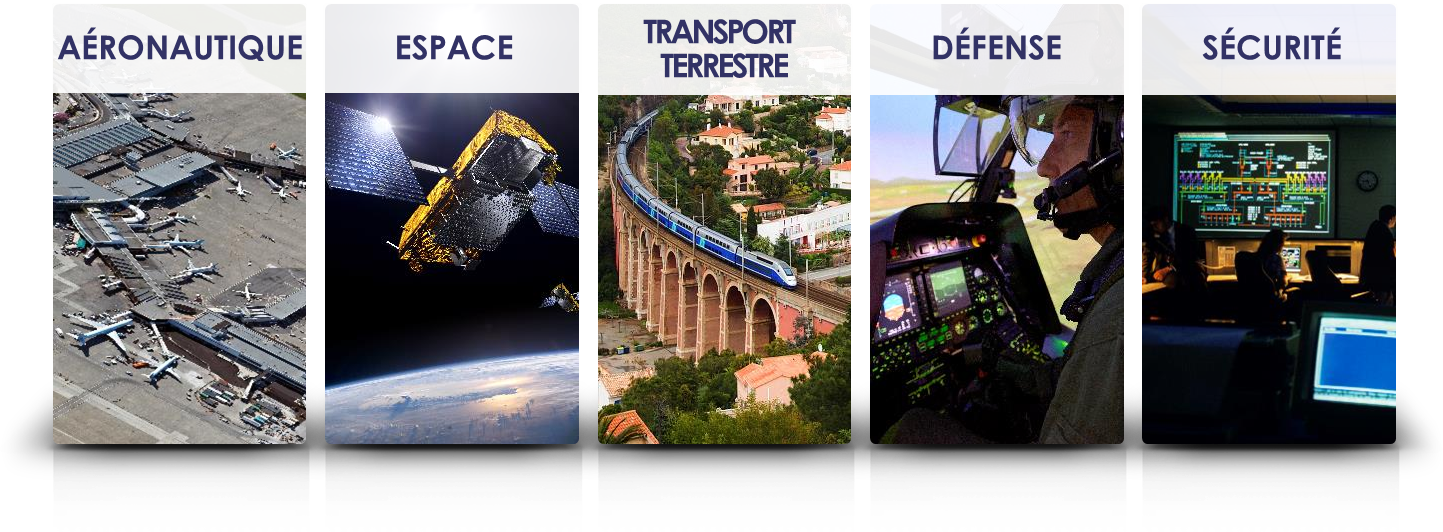
\includegraphics[scale=0.56]{image/thales}
    \caption{Les domaines d'activité du groupe \textbf{\textit{Thales}}.}
    \label{fig:thales}
\end{figure}

\vspace{-0.4 cm}\hspace{-0.5 cm}Les domaines d’activités spécifiques au site de \textit{Tubize} sont la conception et la maintenance de systèmes de communication et d’information :
\begin{itemize}
\item Systèmes de communication : équipements radio HF et VHF robustes et sécurisés (boîtes d’antennes, amplificateurs de puissance, coupleurs d’antennes) pour les communications terrestres, navales ou aéronautique, qu’elles soient civiles ou militaires.
\item Systèmes d’information : dispositifs de gestion d’urgence, d’information aux usagers de transports, BMS (\textit{Battlefield Management System}), soldat modernisé, vétronique (systèmes électroniques de navigation et de communication des véhicules militaires).
\item Protection de l’information : sécurisation des échanges de données et protection contre le vol et la publication de données confidentielles. \\
\end{itemize}


\newpage
%%%%%%%%%%%%%%%%%%%%%%%% Partie 2 - Objectifs du stage %%%%%%%%%%%%%
\section{Objectifs }
\label{sec:objectifs}

 
L'objectif de ce stage était d'introduire l'ensemble des notions élémentaires, nécessaires pour la réalisation du \textit{Travail de Fin d'Étude} (TFE). Ce travail de fin d'étude qui allait se poursuivre durant 6 mois à compter du mois de Novembre 2018. Dans un premier temps, il s'agit donc surtout de définir les concepts théoriques. Ensuite, un exemple ou une simulation est mise en oeuvre afin d'appuyer le concept théorique.\\ \\
La liste ci-dessous reprend l'ensemble des objectifs fixés et réalisés durant les 6 semaines de stage : 
\begin{description}
\item[1. Chiffrement] 
\item[2. L'algorithme AES (\textit{Advanced Encryption Standard})]
\item[3. Introduction aux \textit{Side-Channel Attacks} (attaques par canal auxiliaire)]
\item[4. Cas spécifique des \textit{Side-Channel Attacks} : Attaques \textit{CPA}] 
\item[5. Simulation d'une attaque CPA sur MATLAB] 
\item[6. Contre-mesures] 
\item[7. Simulation contre-mesures sur MATLAB] 
\end{description}
Ces différents objectifs sont décrits dans la section \ref{sec:Projet} \textit{"Projet du stage"}.

%%%%%%%%%%%%%%%%%%%%%%%% Partie 3 - Projet du stage %%%%%%%%%%%%%
\section{Projet du stage}
\label{sec:Projet}

Cette section décrit l'ensemble des objectifs, cités à la section \ref{sec:objectifs}, fixés pour le stage. 

%%%% PARTIE 3.1
\subsection{Notions  de chiffrement}

Les systèmes de sécurité modernes utilisent des algorithmes de chiffrement pour assurer la disponibilité, la confidentialité et l'intégrité de données. Ces algorithmes de chiffrement sont en réalité des fonctions mathématiques qui prennent typiquement : 
\begin{itemize}
\item  2 paramètres en entrée : un \textbf{\textit{message clair}} (nommé \textit{plaintext} en anglais) et une \textbf{\textit{clé de chiffrement}} (nommée \textit{key} en anglais).
\item 1 paramètre en sortie : le \textbf{\textit{message chiffré}} (nommé \textit{ciphertext} en anglais). \\
\end{itemize}
Le procédé transformant les données claires en entrée en données chiffrées en sortie est appelé le \textbf{\textit{chiffrement}}.
Ce procédé est réalisé grâce à un \textbf{\textit{algorithme de chiffrement}} utilisant une clé de chiffrement et diverses opérations mathématiques. Il est important de préciser que tous les détails décrivant le fonctionnement d'un algorithme sont disponibles publiquement, seule la clé de chiffrement doit rester secrète. En effet, la sécurité offerte par un algorithme de chiffrement ne doit pas dépendre du secret de son implémentation. Un bon algorithme est un algorithme dont on ne parviendra pas à déchiffrer les données chiffrées. Lorsque la clé d'un algorithme est trouvée, le déchiffrement des données confidentielles peut être réalisé. On dit que l'algorithme de chiffrement est \textbf{\textit{cassé}}.

La figure \ref{fig:chiffrement} ci-dessous présente le principe de fonctionnement d'un algorithme de chiffrement.

\begin{figure}[htbp]
    \centering
    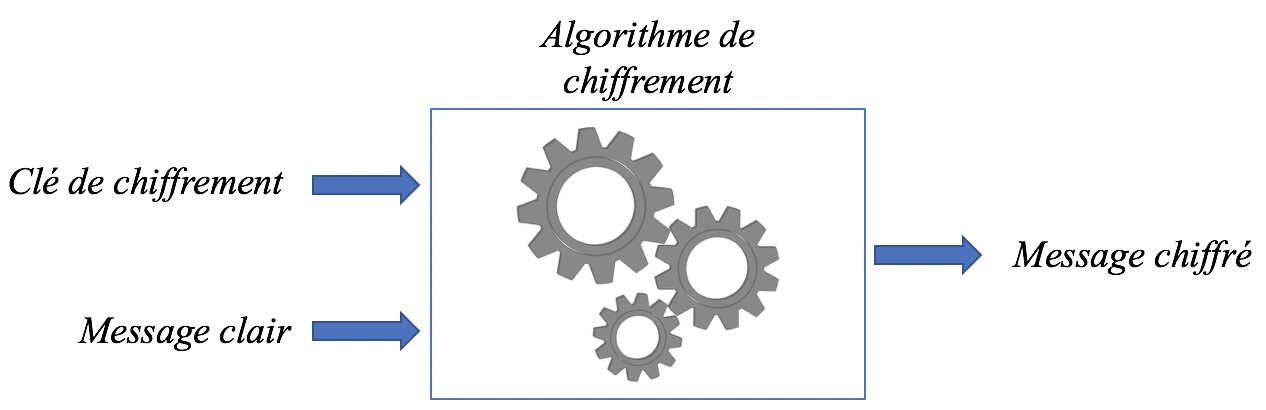
\includegraphics[width=0.7\textwidth]{image/chiffrement}
    \caption{L'algorithme de chiffrement, caractérisé par diverses opérations mathématiques, utilise une clé de chiffrement en entrée pour chiffrer un message clair. Cela produit un message chiffré, non compréhensible pour une personne ne connaissant pas la clé de chiffrement.}
    \label{fig:chiffrement}
\end{figure}

\newpage

Nous distinguons 2 types d'algorithmes de chiffrements : 
\begin{itemize}
\item \textbf{\textit{Chiffrement symétrique}} : Le chiffrement est dit symétrique lorsque le procédé de chiffrement (algorithme) utilise une seule clé, appelée \textit{clé secrète}. Par convention, ce type de chiffrement permet à la fois de chiffrer et de déchiffrer des messages à partir d'une seule et unique clé. Le désavantage de ce typer de chiffrement est que si une personne parvient à subtiliser la clé, elle sera en mesure de déchiffrer tout message qu'elle intercepte.  \\
\textit{Exemple} : L'algorithme AES (\textit{Advanced Encryption Standard}). Une explication plus détaillée de cet algorithme est reprise à la section \ref{sec:AES}
\item \textbf{\textit{Chiffrement asymétrique}} : Le chiffrement est dit asymétrique lorsque le procédé de chiffrement (algorithme) utilise 2 clés : une \textit{clé publique} et une \textit{clé privée}. Par convention, la clé publique est la clé de chiffrement du message clair, elle peut être communiquée sans aucune restriction tandis que la clé privée est la clé de déchiffrement du message chiffré, elle ne doit être communiquée sous aucun prétexte. Le fonctionnement est le suivant : Avec une clé publique, l'expéditeur code, dans un algorithme de chiffrement donné, un message. Ce message, une fois transmis, ne pourra être déchiffré que par le destinataire, détenteur de la clé privée. \\
\textit{Exemple} : L'algorithme RSA (\textit{Rivest Shamir Adleman}). \\
\end{itemize}

Les figures \ref{fig:symétrique} et \ref{fig:asymétrique} ci-dessous présentent les principes de fonctionnement des chiffrements symétriques et asymétriques respectivement.

\begin{figure}[htbp]
    \centering
    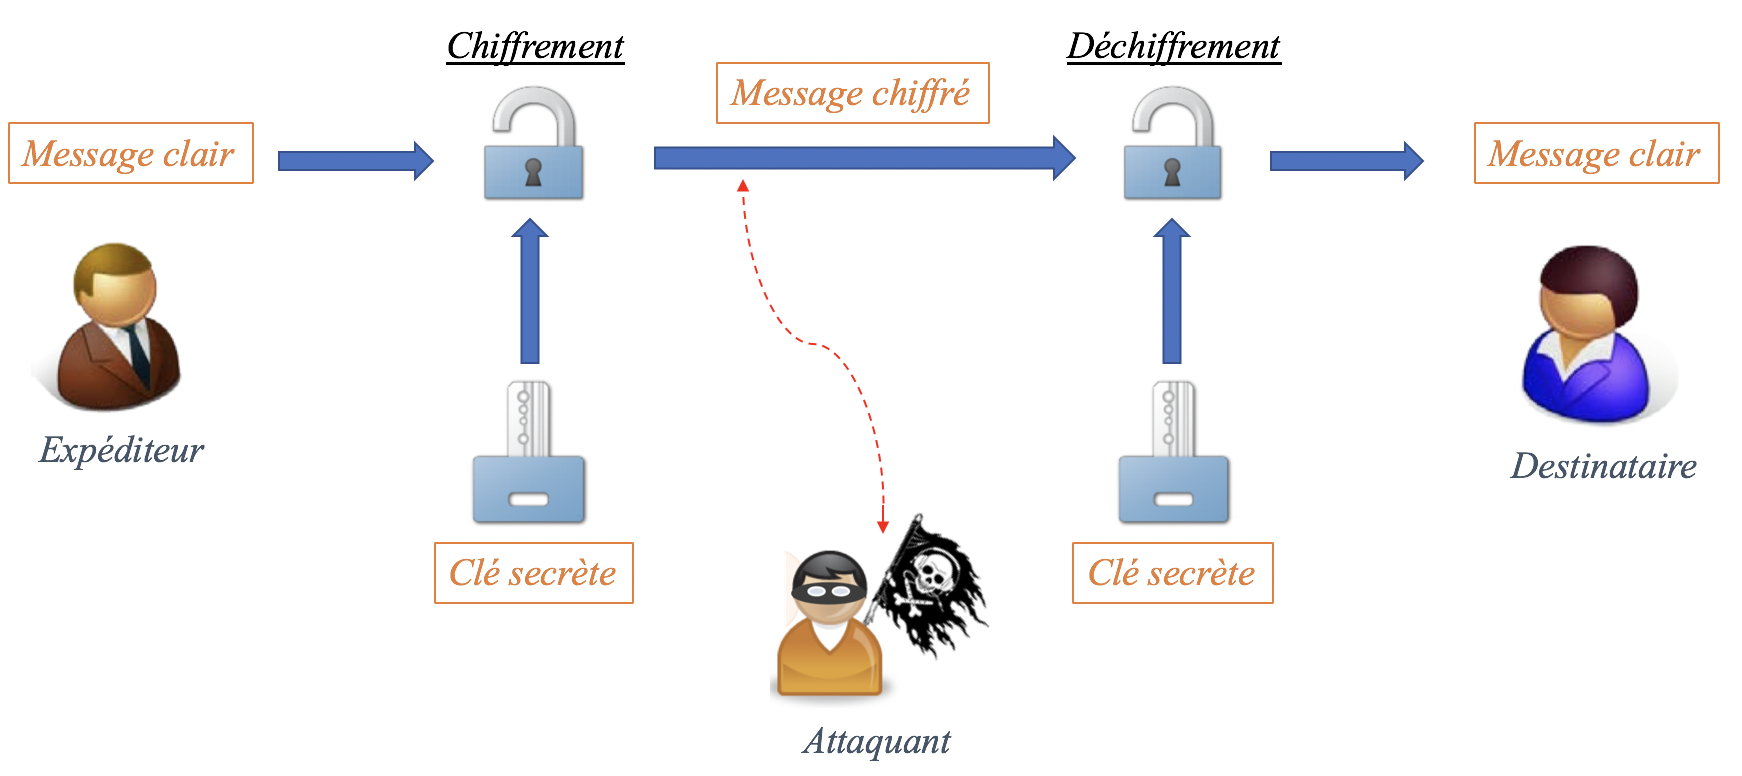
\includegraphics[width=0.65\textwidth]{image/symetrique}
    \caption{Chiffrement symétrique : Une seule clé est utilisée pour chiffrer et déchiffrer les messages.}
    \label{fig:symétrique}
\end{figure}

\begin{figure}[htbp]
    \centering
    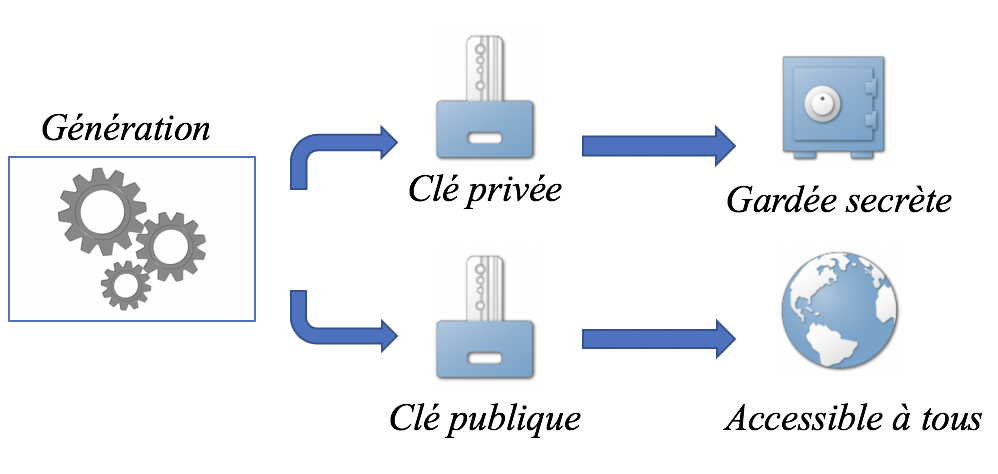
\includegraphics[width=0.38\textwidth]{image/cle_asymetrique}
    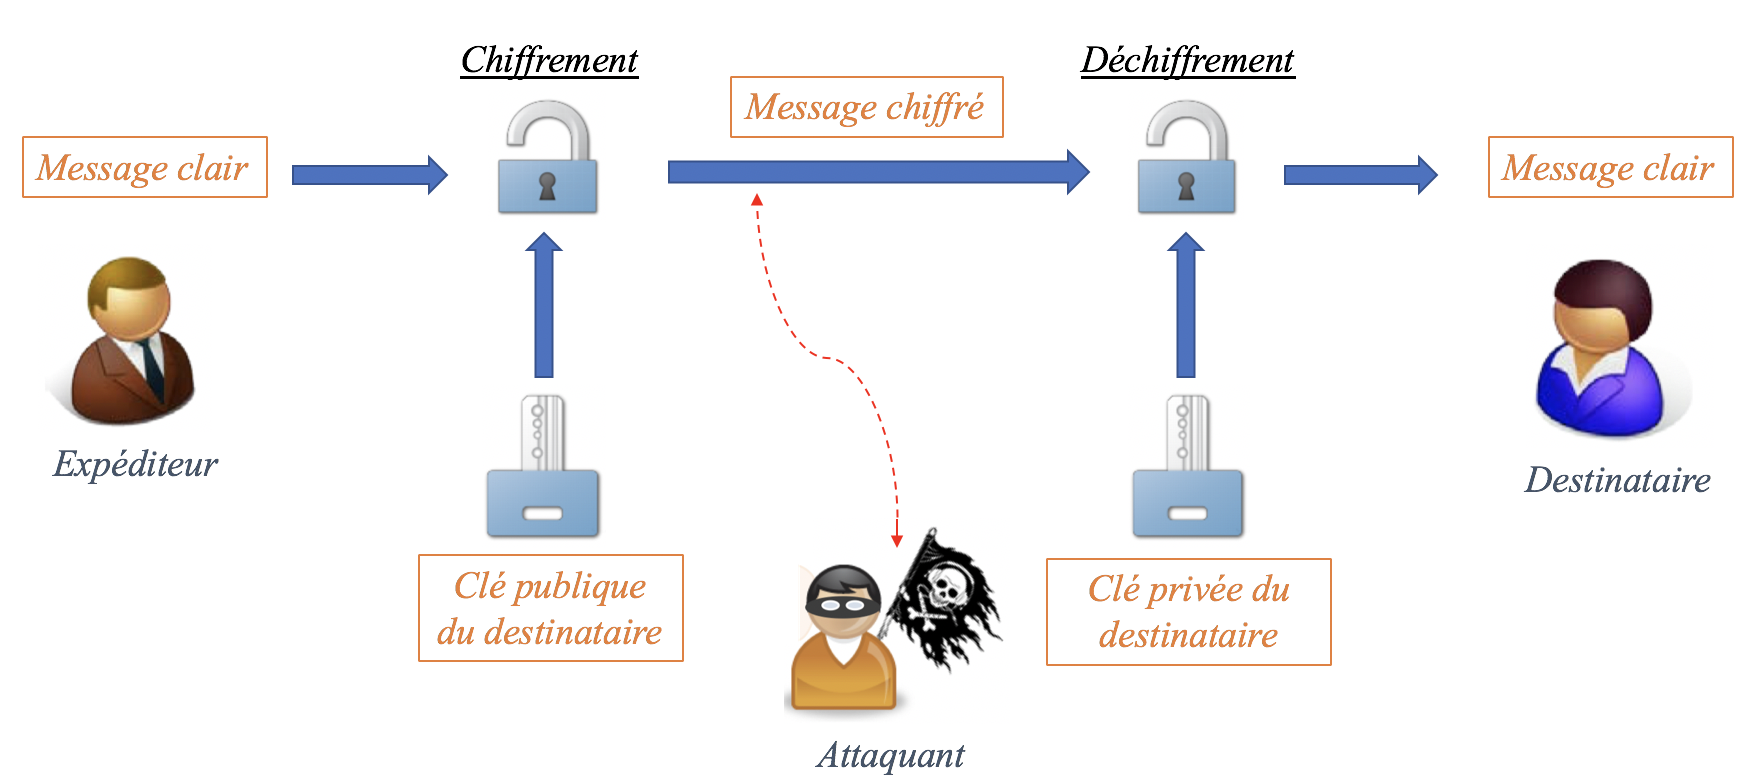
\includegraphics[width=0.7\textwidth]{image/asymetrique}
    \caption{Chiffrement asymétrique : Un clé publique est utilisée pour chiffrer le message et une clé privée est utilisée pour le déchiffrer.}
    \label{fig:asymétrique}
\end{figure}


Que ce soit pour un algorithme de chiffrement symétrique ou asymétrique, la clé de chiffrement doit être stockée sur un support physique. Ce support, appelé \textit{device cryptographique}, doit être suffisamment sécurisé que pour contenir de manière protégée la clé. Ainsi, un \textbf{\textit{device cryptographique}} est un device qui implémente des algorithmes de chiffrement et qui stocke des clés de chiffrement (exemple : \textit{FPGA}).

\subsection{Algorithme \textit{AES} (\textit{Advanced Encryption Standard})}
\label{sec:AES}

En 1997, le NIST (\textit{National Institute of Standards and Technology}) décida qu'il était temps de développer un nouveau standard d'algorithme de chiffrement. Ce nouveau standard, nommé \textbf{AES} (pour \textit{Advanced Encryption Standard}), était appelé à remplacer l'ancien standard de chiffrement, l'algorithme DES (pour \textit{Data Encryption Standard}). Pour ce faire, le NIST organisa un concours cryptographique, les chercheurs du monde entier furent invités à soumettre leurs propositions. En Octobre 2000, Le NIST annonça le vainqueur du concours : l'algorithme de Rijndael, du nom de ses concepteurs Joan Daemen et Vincent Rijmen, tous deux de nationalité belge.

L'algorithme de Rijndael, désormais plus connu sous le nom d'algorithme AES, est un \textbf{algorithme de chiffrement symétrique par blocs}. C'est-à-dire que les données sont traitées par blocs de 128 bits. La clé secrète peut posséder différentes tailles : 128 bits (AES-128), 192 bits (AES-192) ou encore 256 bits (AES-256). À noter qu'en théorie, plus la taille de la clé est élevée, moins il y a de chance de casser l'algorithme cependant,  comme nous le verrons par la suite, avec les attaques par canal auxiliaire (section \ref{sec:att}), le problème peut vite être contourné. La description qui suit est basée sur l'algorithme AES-128 bits, c'est-à-dire que la clé de chiffrement a une taille de 128 bits.

L'AES-128 a donc pour rôle de chiffrer des blocs de données de 128 bits avec une clé de 128 bits. Les données et la clé sont représentés par une matrice où chaque élément de la matrice correspond à un byte (un octet, i.e 8 bits). Étant donné que 128 bits correspond à 16 bytes, la matrice de données, au même titre que la matrice de clé, correspond à une matrice de 4 lignes et 4 colonnes (formant ainsi les 4x4 soit 16 bytes). Une matrice particulière (de taille 4x4 également) appelé STATE contient l'ensemble des résultats intermédiaires résultant des diverses opérations que subissent les données (depuis leur état initial). 

La figure \ref{fig:matrix} présente les 3 matrices qui viennent d'être citées : la matrice de donnée (message clair initial de 128 bits), la matrice STATE (qui va contenir les résultats intermédiaires des données suite aux différentes opérations) et la matrice clé (clé de 128 bits).
\begin{figure}[htbp]
    \centering
    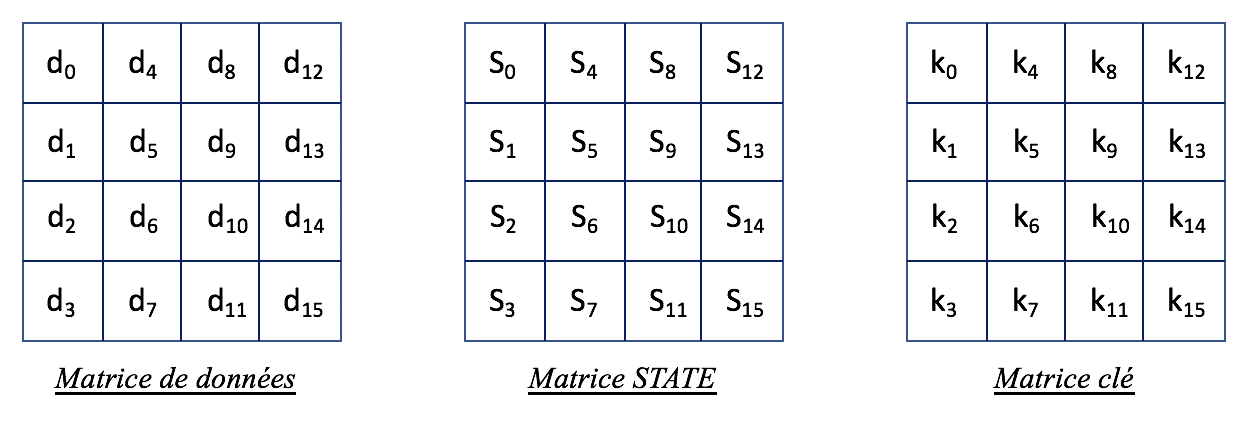
\includegraphics[scale=0.75]{image/matrix}
    \caption{Les 3 matrices utilisées par l'algorithme AES.}
    \label{fig:matrix}
\end{figure}

\textit{Remarque} : En pratique, la matrice de données est directement confondue avec la matrice STATE. Autrement dit, les premiers éléments à être placés dans la matrice STATE représentent les bytes de données. Ainsi, on n'utilise que deux matrices durant le fonctionnement de l'algorithme AES : la matrice STATE et la matrice clé.

Par ailleurs, l'algorithme AES est caractérisé par une série de tours (\textit{rounds} en anglais) dépendant de la taille de la clé. Pour une clé dont la taille est 128 bits, on dénombre 10 tours (12 tours pour une clé de 192 bits et 14 tours pour une clé de 256 bits). Un tour est définit par 4 opérations appliquées succinctement sur la matrice STATE. Ces 4 opérations sont : \textit{AddRoundKey}, \textit{SubBytes}, \textit{ShiftRows} et \textit{MixColumns}. Elles sont appliquées à divers instants dans l'exécution de l'algorithme AES. La figure \ref{fig:AES} (page suivante) permet de visualiser l'ordre d'exécution chronologique de ces 4 opérations. L'annexe \ref{ann:AES} reprend quant à elle le code réalisé pour l'exécution de l'algorithme AES-128.

\newpage

La figure \ref{fig:AES} ci-dessous présente le principe de fonctionnement général de l'algorithme AES-128.
\begin{figure}[htbp]
    \centering
    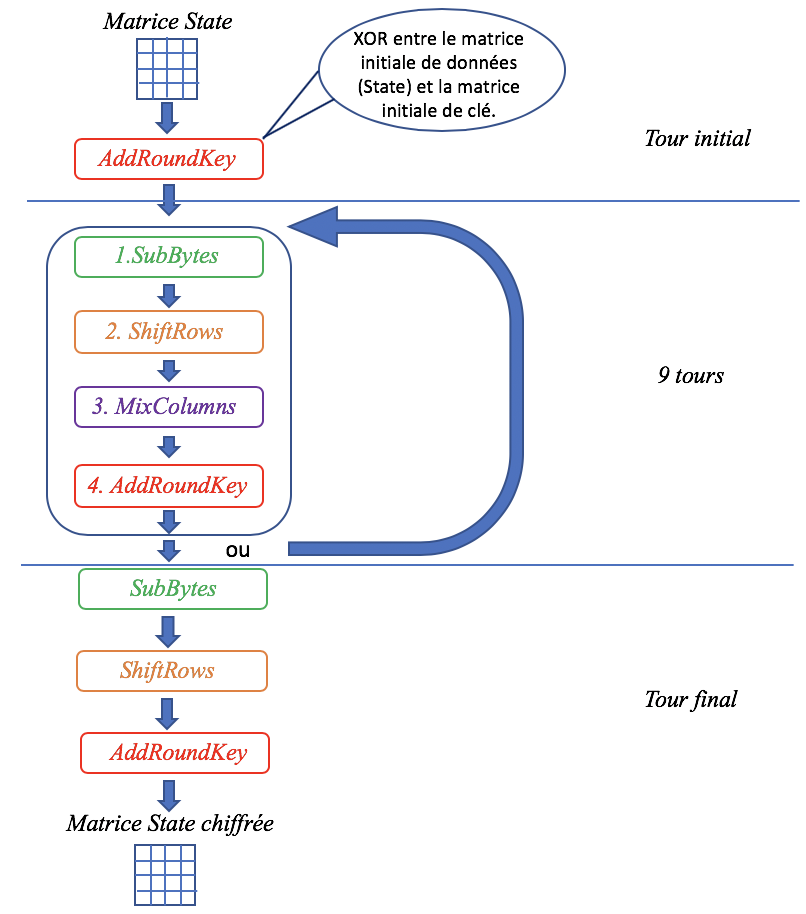
\includegraphics[scale=0.75]{image/AES}
    \caption{Principe de fonctionnement de l'algorithme AES-128.} 
    \label{fig:AES}
\end{figure}



\underline{\textbf{Fonctionnement :}} 

Initialement, deux matrices vont être utilisées : la matrice STATE, contenant les données claires, et la matrice clé, contenant la clé secrète initiale. La première opération à être appliquée sur ces deux matrices est l'opération \textit{AddRoundKey}. Cette opération réalise un XOR (symbole \oplus) entre chaque élément de la matrice STATE et chaque élément respectif de la matrice clé. Le résultat est ré-écrit dans la matrice STATE. La figure \ref{fig:XOR} ci-dessous présente le principe de fonctionnement de cette première opération :
\begin{figure}[htbp]
    \centering
    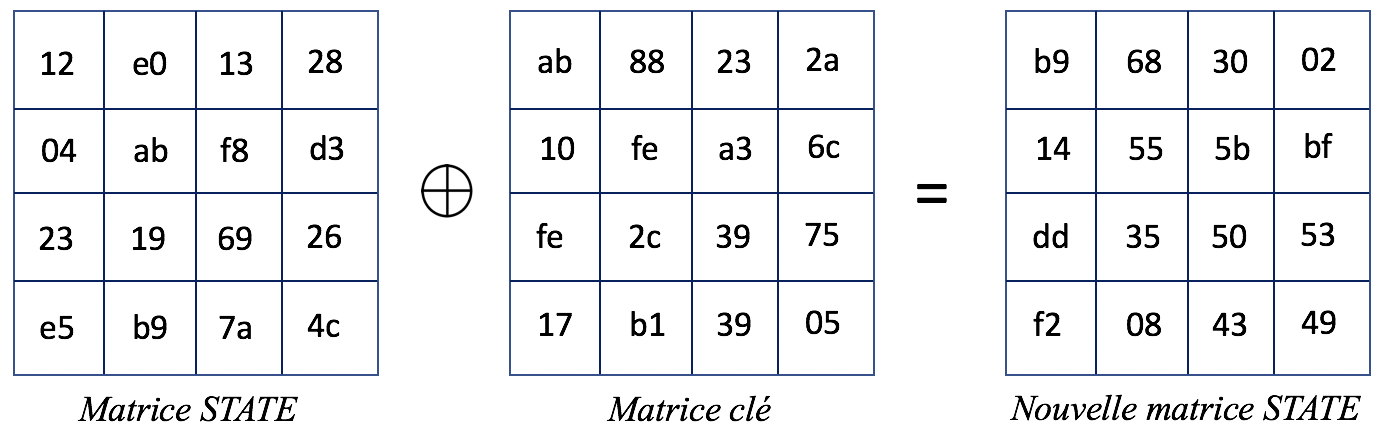
\includegraphics[scale=0.55]{image/XOR}
    \caption{Opération \textit{AddRoundKey} entre la matrice STATE et la matrice clé.}
    \label{fig:XOR}
\end{figure}

\hspace{-0.5 cm}Ensuite, une série de quatre opérations se répétant neuf fois (9 tours cycliques) est exécutée. Ces quatres opérations sont appliquées dans l'ordre suivant : \textit{SubBytes}, \textit{ShiftRows}, \textit{MixColumns}, \textit{AddRoundKey}. \\
Enfin, une fois les neufs tours exécutés, le neuvième et dernier \textit{round} se lance exécutant trois opérations : \textit{SubBytes}, \textit{ShiftRows} et \textit{AddRoundKey}. À la fin de ces trois dernières opérations, une matrice de taille 4x4 (la matrice STATE) présente le message chiffré de 128 bits.


\underline{\textbf{Description des 4 opérations :}} \\
\begin{description}
\item[1. SubBytes] : 
La figure \ref{fig:SubBytes} ci-dessous présente le principe de fonctionnement de l'opération \textit{SubBytes}. Le principe de fonctionnement présenté dans ce cas-ci est simple : il repose sur une table de substitution, appelée Sbox et présentée en annexe \ref{ann:Sbox}. La matrice STATE avant l'exécution de l'opération contient 16 bytes. Chacun de ses 16 bytes (notés $S_{i,j}$) va fournir une nouvelle valeur de byte (noté $S'_{i,j}$) en fonction de la Sbox. Un exemple est donné afin de comprendre le principe : Si le byte $S_{1,2}$ vaut $53$ (hexa) alors, selon la Sbox, la valeur du byte résultant $S'_{1,2}$ vaut $ed$ (hexa).

\begin{figure}[htbp]
    \centering
    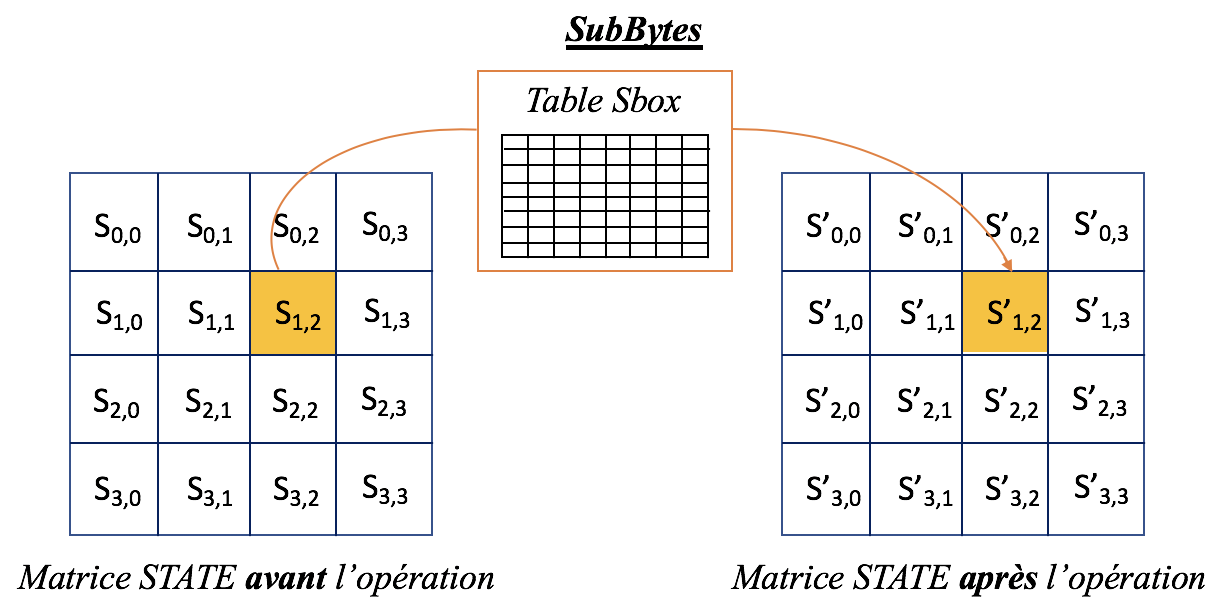
\includegraphics[scale=0.42]{image/SubBytes}
    \caption{Opération \textit{SubBytes} exécutée sur la matrice STATE.}
    \label{fig:SubBytes}
\end{figure}

\item[2. ShiftRows] : Comme son nom l'indique, cette opération concerne les lignes de la matrice STATE. Cette opération réalise une permutation cyclique des octets sur les lignes de la matrice STATE. Plus précisément, \textbf{pour la \textit{i-ième} ligne, on décalera chaque élément de la matrice STATE de \textit{i} positions vers la gauche}, en considérant que la première ligne a pour indice 0.
La figure \ref{fig:ligne} ci-dessous présente le principe de fonctionnement de l'opération \textit{ShiftRows} :
\begin{figure}[htbp]
    \centering
    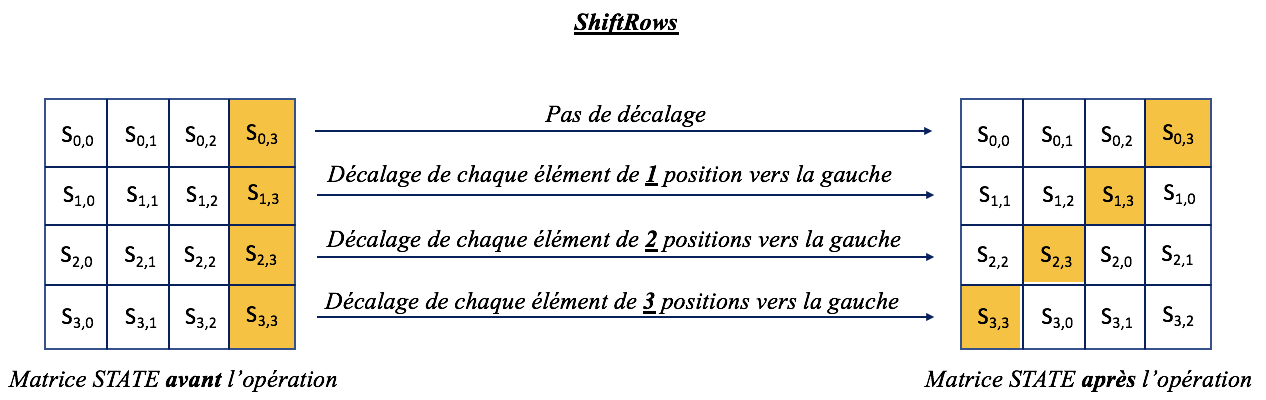
\includegraphics[scale=0.55]{image/ligne}
    \caption{Opération \textit{ShiftRows} exécutée sur la matrice STATE.}
    \label{fig:ligne}
\end{figure}

\item[3. MixColumns] : Comme son nom nom l'indique, cette opération concerne les colonnes de la matrice STATE. \textbf{Cette opération réalise un produit matriciel entre une matrice fixée (taille 4x4) définie ci-dessous} (figure \ref{fig:colonnebis}) \textbf{et un vecteur colonne (taille 4x1) de la matrice STATE}. Cela produit un nouveau vecteur colonne (taille 4x1) permettant de définir la nouvelle matrice STATE.
La figure \ref{fig:colonne} ci-dessous présente le principe de fonctionnement de l'opération \textit{MixColumns}. Un exemple est ensuite donné à la figure \ref{fig:colonnebis}.
\begin{figure}[htbp]
    \centering
    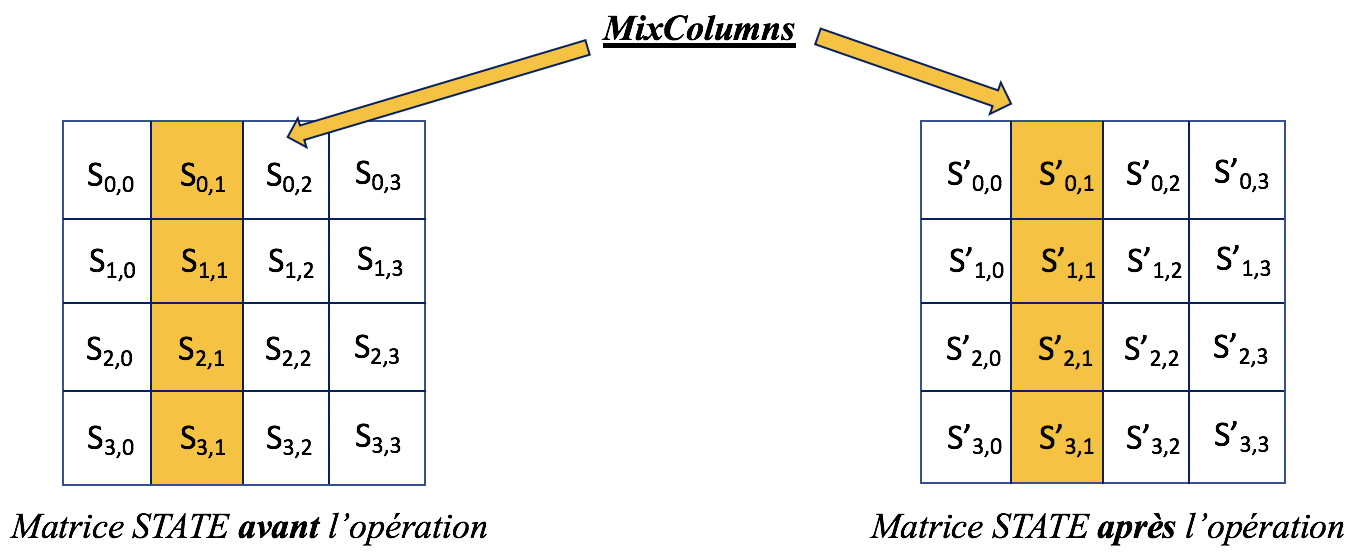
\includegraphics[scale=0.42]{image/colonne}
    \caption{Opération \textit{MixColumns} exécutée sur la matrice STATE.}
    \label{fig:colonne}
\end{figure}
\begin{figure}[htbp]
    \centering
    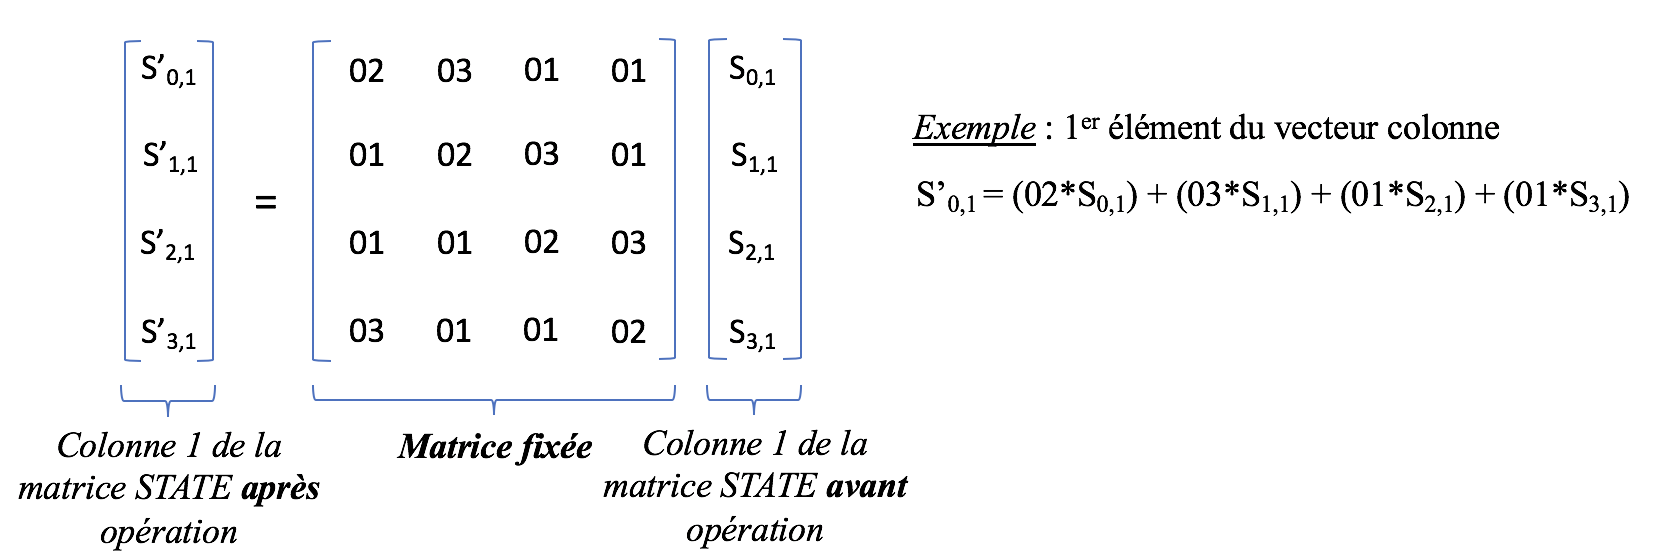
\includegraphics[scale=0.54]{image/colonnebis}
    \caption{Exemple de l'opération \textit{MixColumns} exécutée sur la deuxième colonne (i.e colonne 1) de la matrice STATE.}
    \label{fig:colonnebis}
\end{figure}

\item[4. AddRoundKey] : La gestion des clés se fait au travers des fonctions \textit{AddRoundKey} et \textit{KeySchedule}. Comme précisé précédemment dans le fonctionnement initial, l'opération \textit{AddRoundKey} réalise un simple XOR entre la matrice STATE et la matrice de clé. Le résultat de ce XOR est placé dans la nouvelle matrice STATE.\\ 
On sait que la matrice STATE est modifiée après chaque opération exécutée. Ce qu'on ne sait pas encore, c'est que la matrice clé est également modifiée à chaque round afin d'éviter d'utiliser toujours la même valeur de clé. Cela permet ainsi de complexifier le chiffrement des données. L'opération qui modifie la matrice de clé initiale en une nouvelle matrice de clé est appelée \textbf{\textit{KeySchedule}}. Cette opération génère une nouvelle clé sur base de la clé précédemment employée. Ainsi, pour générer la première nouvelle clé, l'opération \textit{KeySchedule} emploiera la clé initialement donnée. Étant donné que pour l'AES-128, nous avons un total de dix rounds à exécuter, cela signifie que l'opération \textit{KeySchedule} s'exécute dix fois afin de générer dix nouvelles clés de 128 bits. En rajoutant la clé initiale, nous aurons alors onze clés de chiffrement différentes permettant d'exécuter les onze opérations \textit{AddRoundKey} présentes dans l'algorithme AES-128. Ainsi, comme présenté à l'annexe \ref{ann:AES}, l'opération \textit{KeySchedule} s'exécute en premier lieu dans le code afin de générer dix nouvelles clés. En comptant la clé initialement donnée, il y a donc onze clés. Chacune de ces onze clés sera utilisée lors de l'appel de la fonction \textit{AddRoundKey}.\\ 

La figure \ref{fig:XOR} reste inchangée pour décrire le principe de fonctionnement de l'opération \textit{AddRoundKey}. Nous rappelons toutefois que la matrice clé est bien modifiée lors de chaque exécution de cette opération. \\
L'annexe \ref{ann:KeySchedule} permet quant à elle de comprendre le principe de fonctionnement de l'opération \textit{KeySchedule}, utilisée afin de générer les nouvelles clés. Plus précisément, cette annexe présente un exemple pour générer la première nouvelle clé. \\ \\
Le fonctionnement est le suivant : l'opération \textit{KeySchedule} s'exécute colonne par colonne (sur la matrice clé de taille 4x4). On va d'abord générer la première colonne de la nouvelle clé, ensuite on générera les colonnes 2, 3 et 4. C'est la première colonne qui est la plus compliquée à générer. Les 3 autres colonnes réalisent simplement un XOR pour générer la nouvelle colonne.
Ainsi, pour obtenir la 1ère colonne de la nouvelle clé (soit les quatre 1ers bytes), on va prendre 3 vecteurs colonnes (taille 4x1) : 
\begin{enumerate}
\item Prendre la 4ème colonne de la clé initiale.
\begin{enumerate}
\item Décaler chaque élément de cette colonne d'une position vers le haut.
\item Appliquer l'opération \textit{SubBytes} sur chaque élément de la colonne.
\end{enumerate}
\item Prendre la 1ère colonne de la clé initiale.
\item Prendre la 1ère colonne de la matrice RCON.
\end{enumerate}
Une fois ces trois vecteurs colonnes obtenus, on réaliser un XOR entre eux. Le résultat de ce XOR représente la 1ère colonne de la nouvelle matrice clé. Une fois ce





\end{description}


\newpage

\subsection{Introduction aux \textit{attaques par canal auxiliaire}}
\label{sec:att}
\subsubsection{Types d'attaques}

A la fin des années 1990, une nouvelle contrainte pour la conception de système informatique a vu le jour : la sécurité matérielle. Bien souvent, la sécurité d'un système informatique s'appuie plus sur les concepts software que hardware. Cependant, un nouveau mode d'attaque s'est développé. Il s'agit d'attaques physiques, c'est-à-dire d'attaques réalisées sur le circuit électronique lui-même. Deux grandes familles d'attaques sont recensées : 
\begin{itemize}
\item \textbf{\textit{Attaques actives}} : Une attaque est dite active lorsque les entrées et/ou l'environnement du device cryptographique sont manipulés par l'attaquant en vue de produire un comportement anormal du device. La clé secrète est révélée en exploitant les données issues de ce comportement anormal. Cela peut être une variation de la tension du device, une injection de glitch d'horloge, etc. On distingue deux types d'attaques actives : 
\begin{itemize}
\item Les attaques actives \textbf{\textit{irréversibles}} qui conduisent à la destruction du device cryptographique. Ce type d'attaque est souvent réalisé pour connaître la conception physique d'un device. \textit{Exemple} : Découpage laser d’un circuit intégré.
\item Les attaques actives \textbf{\textit{pseudo-réversibles}} qui n’entrainent pas forcément la destruction du device cryptographique, mais qui sont souvent tout de même invasives puisqu’elles nécessitent la préparation du circuit (découpe partielle du boitier du circuit intégré par exemple). Un exemple typique de ce type d'attaque est ce qu'on appelle les \textit{attaques en fautes}. Le principe est d'introduire volontairement des fautes dans le circuit (exemple : Injection de rayon laser, injection de glitch d’horloge, etc.). Les fautes ainsi créées peuvent entrainer le circuit dans des modes de fonctionnement conduisant à des erreurs. Ces erreurs peuvent ensuite être exploitées pour déterminer la clé.
\end{itemize}
\item \textbf{\textit{Attaques passives}} : Une attaque est dite passive lorsque l'attaquant exploite l'analyse, en fonctionnement normal, d'informations s'échappant d'un device cryptographique. Cela peut être l'analyse de la consommation de puissance, l'analyse temporelle, l'analyse par rayonnement électromagnétique, etc. C'est ce type d'attaque qui sera détaillé tout au long de ce stage et durant la réalisation de TFE. \\
\end{itemize}

\vspace{-0.1 cm}La figure \ref{fig:attaques} ci-dessous résume les différents types d'attaques physiques possibles.
\begin{figure}[htbp]
    \centering
    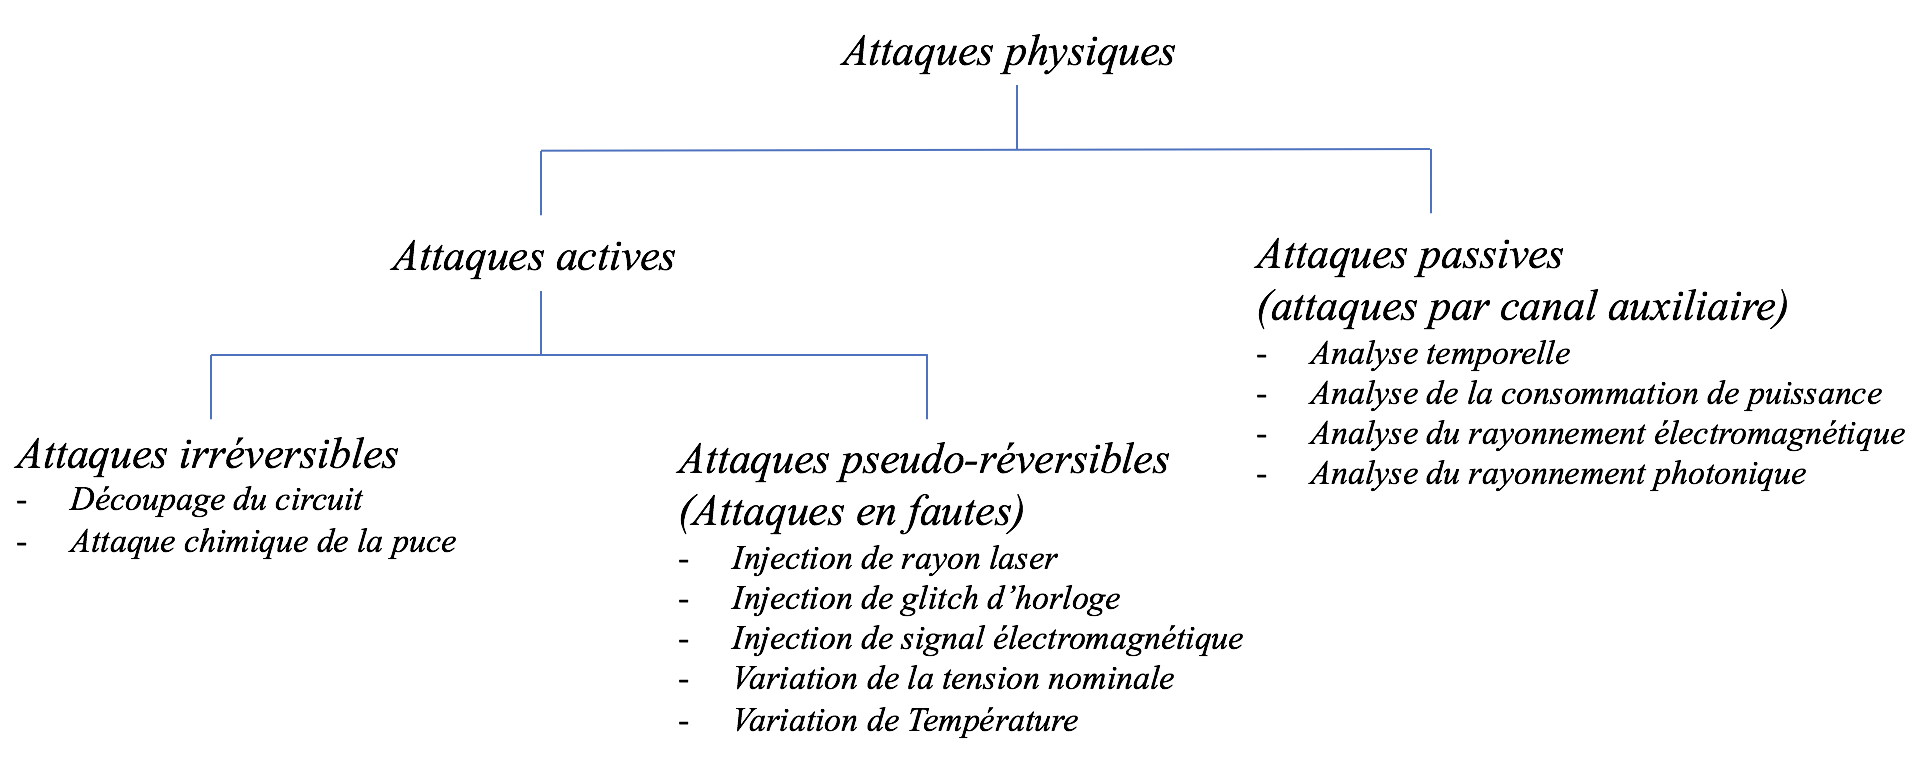
\includegraphics[width=0.9\textwidth]{image/attaques}
    \caption{Les 2 grandes familles d'attaques physiques possibles. La suite de ce rapport se concentre essentiellement sur les attaques physiques dites passives.}
    \label{fig:attaques}
\end{figure}

\vspace{-0.2 cm}Les attaques passives sont globalement beaucoup plus simples à mettre en oeuvre que les attaques actives. Comme définit précédemment, ces attaques consistent à analyser des données issues de canaux auxiliaires au device cryptographique (lorsque ce dernier est en état de fonctionnement normal). Ces canaux auxiliaires sont des canaux présents physiquement sur le circuit attaqué et le long desquels de l’information s’échappe (sous différentes formes : rayonnement électromagnétique, rayonnement photonique, consommation de puissance, etc.). C'est là qu'intervient la notion de \textit{side-channel attacks} ou en français \textit{l'attaque par canal auxiliaire}. 
En effet, les fonctions cryptographiques, bien que pouvant être extrêmement robustes théoriquement (c'est-à-dire mathématiquement) sont très sensibles aux fuites d’informations. C'est-à-dire qu'une quantité très faible d’informations peut être exploitée pour casser un algorithme cryptographique très fort. C’est ce que les attaques par canaux auxiliaires exploitent. 

La figure \ref{fig:attackpassive} ci-dessous présente les différentes façons possibles de réaliser des attaques passives.
\begin{figure}[htbp]
    \centering
    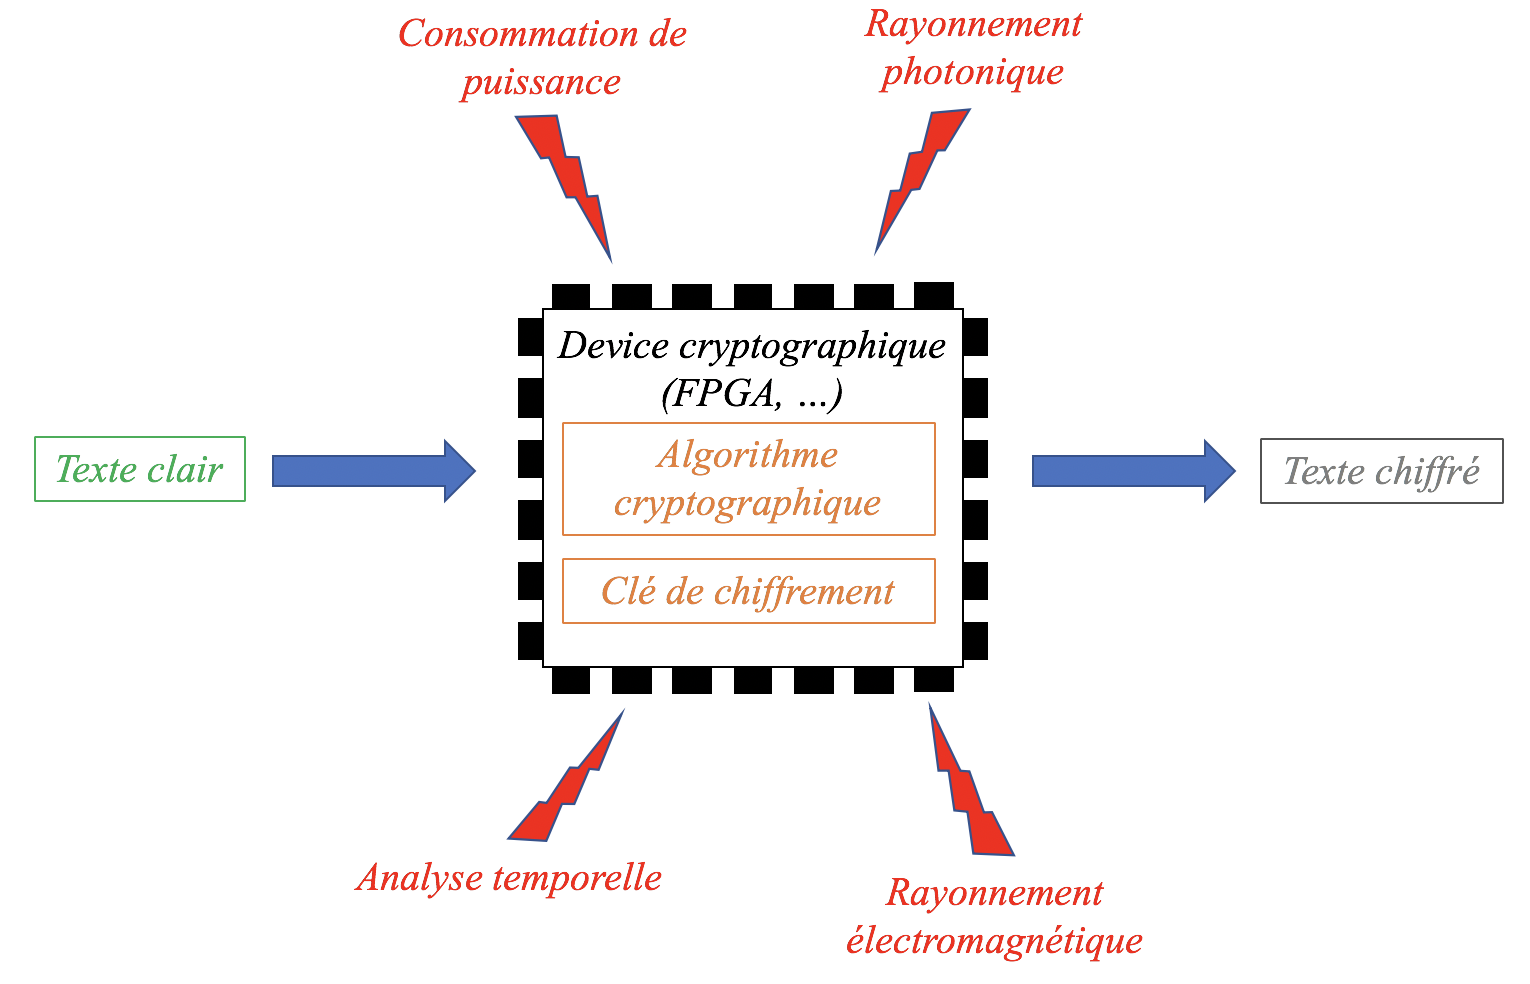
\includegraphics[scale=0.4]{image/attackpassive}
    \caption{Les différentes façons d'attaquer passivement un device cryptographique en vue de casser l'algorithme de chiffrement qui se trouve dessus.}
    \label{fig:attackpassive}
\end{figure}

Dans la suite de cet ouvrage, on se concentrera sur un type précis d'attaque passive : l'attaque sur \textbf{l'analyse de la consommation de puissance}. Les sections suivantes décrivent le principe de fonctionnement de ce type d'attaque. 

\subsubsection{Introduction aux attaques par analyse de la consommation de puissance}

Nous allons donc étudier un cas précis d'attaque passive : l'attaque par \textbf{l'analyse de la consommation de puissance}. Comme son nom l'indique, ce type d'attaque analyse la consommation de puissance du device cryptographique attaqué pour retrouver des informations sensibles. En effet, la consommation de courant d'un circuit électronique dépend de deux facteurs : 
\begin{itemize}
\item Les opérations qui sont exécutées.
\item Les données qui sont manipulées.
\end{itemize}
Ainsi, en mesurant un certain nombre de fois la consommation de puissance d'un circuit, il est possible de retrouver certaines informations comme les opérations exécutées (afin d'identifier un algorithme par exemple), les informations secrètes complètes (clé de chiffrement) ou partielles (poids de Hamming d'une clé de chiffrement). Pour ce faire, un oscilloscope est utilisé afin de capturer et d'enregistrer des données, appelées \textbf{\textit{traces}}, mesurées à partir des canaux auxiliaires du circuit électronique (dans notre cas, un FPGA). Pour réaliser la mesure, une résistance sera placée en série avec un canal du device cryptographique afin que l'oscilloscope soit capable de capturer une différence de potentielle minime. En effet, étant donné que les courants qui circulent sur le device cryptographique sont de valeurs très faibles (\si{\micro}A), un amplificateur est utilisé afin d'amplifier la différence de potentielle. La figure \ref{fig:oscillo} ci-dessous présente le principe de mesure à l'oscilloscope.
\begin{figure}[htbp]
    \centering
    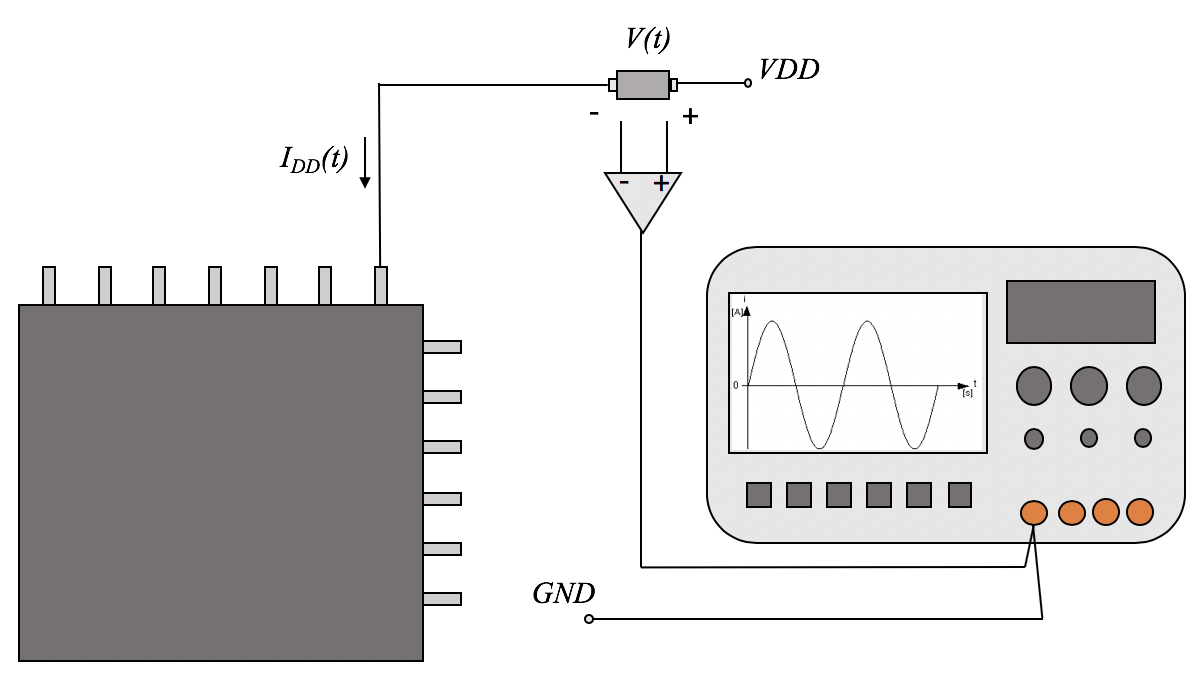
\includegraphics[scale=0.4]{image/oscillo}
    \caption{Principe de mesure à l'oscilloscope.}
    \label{fig:oscillo} 
\end{figure}

\hspace{-0.5 cm}Il existe différents types d'attaques par analyse de la consommation de puissance : 
\begin{itemize}
\item Les attaques SPA (\textit{Simple Power Analysis})
\item Les attaques DPA (\textit{Differential Power Analysis})
\item Les attaques CPA (\textit{Correlation Power Analysis}) \\
\end{itemize}
Nous allons en définir une plus précisément, c'est l'attaque CPA. C'est ce type d'attaque qui a été mis en place durant le stage afin de tenter de casser l'algorithme AES. Ainsi, en continuant l'introduction sur les attaques par analyse de la consommation de puissance, et en prenant le cas particulier d'une attaque dite CPA, nous pouvons dire que : \\ En supposant connu les messages clairs envoyés au device cryptographique et en supposant que ce dernier implémente l'algorithme AES, nous simulerons sur ordinateur le poids de Hamming de chaque donnée binaire obtenue en sortie de l'opération \textit{SubBytes}. Ensuite, nous calculerons les différentes valeurs de coefficient de corrélation entre les traces de puissance capturées à l'oscilloscope et le poids de Hamming obtenu par simulation (sur ordinateur). Sur base de cette étude de la corrélation, nous serons (en principe) capable de déterminer la clé secrète, c'est-à-dire casser l'algorithme AES et ainsi exploiter les données confidentielles. La figure \ref{fig:CPA} présente vulgairement le principe général d'une attaque CPA.
\begin{figure}[h]
    \hspace{-1.5 cm}
    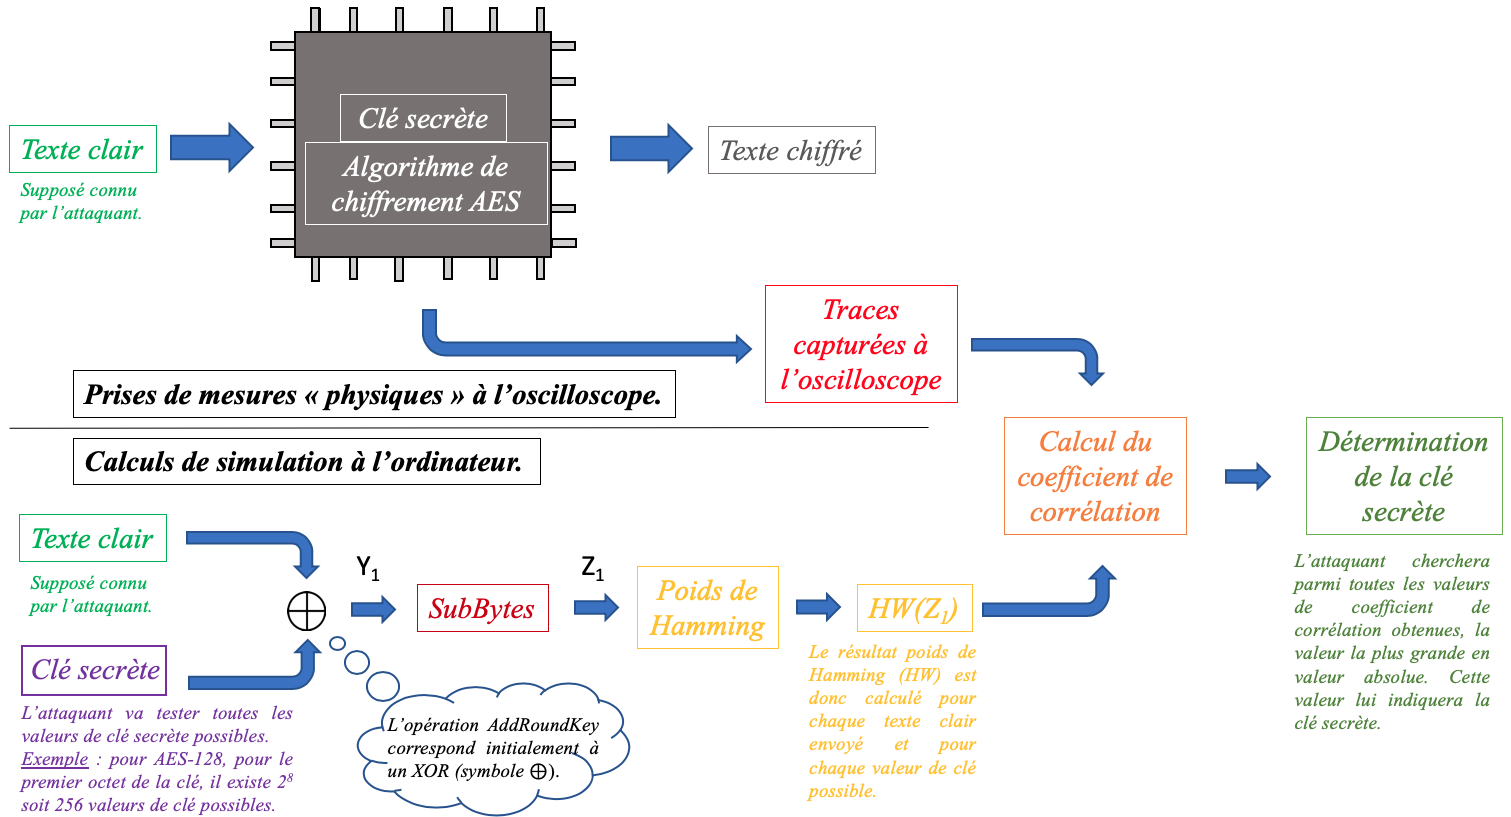
\includegraphics[scale=0.55]{image/CPA}
    \caption{Principe générale d'une attaque CPA.}
    \label{fig:CPA} 
\end{figure}

Le principe d'une attaque par consommation de puissance, et plus particulièrement d'une attaque CPA, ayant été introduit de manière générale, nous allons maintenant revenir sur différentes notions citées ci-dessus afin de mieux les définir et ainsi mieux comprendre le raisonnement qui se cache derrière une attaque par calcul de corrélation (CPA).

\newpage

\subsection{Attaque CPA (\textit{Correlation Power Analysis})}

\subsubsection{Technologie CMOS}
\label{sec:CMOS}
La \textbf{\textit{technologie CMOS}} (pour \textit{Complementary MOS}) est la technologie la plus répandue parmi toutes les technologies de semi-conducteurs. En effet, on la retrouve dans la majorité des systèmes informatiques modernes. En 2001, elle englobait 86\% de la production mondiale des circuits intégrés. Pour cette raison, nous nous intéressons à leur conception afin de détecter des anomalies qui pourraient se révéler être utiles pour la cryptanalyse. Le nom de cette technologie vient du fait que toutes les fonctions logiques (portes OR, NAND, etc.) peuvent être réalisées moyennant l’utilisation d’une paire de transistors MOS complémentaires (N-MOS et P-MOS) associés symétriquement et fonctionnant en régime de commutation. Ainsi lorsqu'un des deux transistor MOS conduit, l’autre est par conséquent fermé. Grâce à ce principe, une porte logique CMOS ne consomme de l’énergie qu’au moment de la commutation. Cette caractéristique permet de distinguer le CMOS de toutes les autres technologies.

\hspace{-0.5 cm}Pour expliquer le fonctionnement de cette technologie, on peut prendre un exemple simple : \textbf{\textit{l'inverseur CMOS}}. Un inverseur CMOS est simplement une fonction \textit{NON}. Voici donc sa table de vérité :
\begin{figure}[htbp]
    \centering
    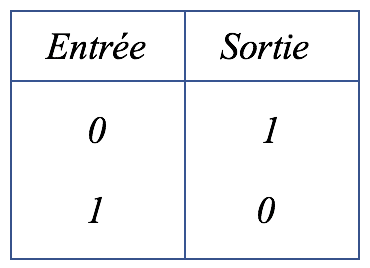
\includegraphics[scale=0.5]{image/verite}
    \caption{Table de vérité pour la fonction NON (inverseur CMOS).}
    \label{fig:verite} 
\end{figure}

\hspace{-0.5 cm}La figure \ref{fig:CMOS} ci-dessous présente le schéma de l'inverseur CMOS :
\begin{figure}[htbp]
    \centering
    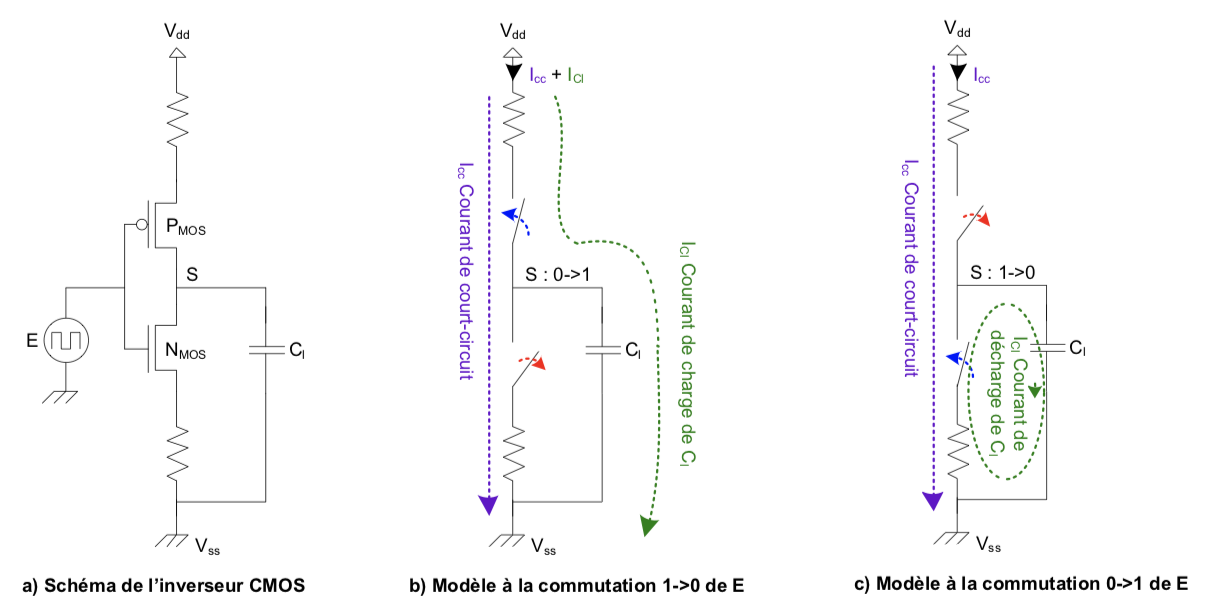
\includegraphics[scale=0.8]{image/CMOS}
    \caption{Schéma de l'inverseur CMOS.}
    \label{fig:CMOS} 
\end{figure}

Si on applique à l'entrée un niveau haut, le transistor N est passant et le P est bloqué. On place ainsi la sortie au potentiel Vss (la masse), c'est-à-dire à l'état bas. Inversement, quand on met l'entrée à l'état bas, le transistor P est passant et le N est bloqué. La sortie est donc à l'état haut. On a donc bien réalisé une fonction inversion.


\subsubsection{Puissance statique et dynamique}
\label{sec:puissance}
Il est évident que les circuits digitaux modernes consomment de la puissance lorsqu'ils exécutent des instructions (opérations) sur des données. Dans le domaine de la cryptanalyse, cette puissance va être mesurée et analysée afin de déterminer si le device cryptographique est attaquable ou non. Dans cette section, nous allons étudier plus particulièrement la consommation de puissance d'un type précis de circuit : les circuits utilisant la technologie CMOS (voir section \ref{sec:CMOS} pour plus de précision). Cette technologie est très répandue et couvre la plupart des circuit digitaux modernes. 

La consommation totale de puissance d'un circuit CMOS peut être obtenue en sommant les consommations de puissance respectives de chaque cellule logique du circuit CMOS. De cette façon, la consommation de puissance totale dépend essentiellement du nombre de cellules logiques dans le circuit CMOS. \\
En prenant comme exemple de cellule logique CMOS, l'inverseur CMOS (expliqué à la section \ref{sec:CMOS}), nous allons tenter de comprendre quand et pourquoi ces cellules CMOS dissipent de la puissance. Pour ce faire, il faut savoir que la consommation de puissance est essentiellement divisée en deux parties : 
\begin{itemize}
\item La puissance statique (notée $P_{stat}$): C'est la puissance qui est consommée lorsqu'il n'y a pas de commutation dans une cellule (c'est-à-dire dans l'inverseur). Autrement dit, c'est la puissance qui est consommée lorsque l'inverseur est en fonctionnement normal mais ne commute pas.
\item La puissance dynamique (notée $P_{dyn}$) : C'est la puissance qui est consommée par une cellule si la sortie de cette cellule commute. 
\end{itemize}
Ainsi, la puissance totale consommée par une cellule vaut la somme de ces deux composantes, soit :
\begin{gather}
	P_{total} = P_{stat} + P_{dyn}
\end{gather}

Mais de façon plus précise, que vaut la puissance statique ? De même, comment pourrait-on exprimer la puissance dynamique ? 

\underline{\textbf{\textit{Puissance statique :}}} \\ \\
Les cellules CMOS sont toujours construites de façon à ce que les deux transistors complémentaires ne soient jamais passants au même moment. En effet, si on reprend l'exemple de l'inverseur CMOS (\ref{sec:CMOS}), lorsqu'on met le signal d'entrée à \textit{GND} alors le transistor P1 est passant et N1 est bloqué. Par contre, lorsqu'on met le signal d'entrée à \textit{$V_{DD}$}, le transistor P1 devient bloqué tandis que le transistor N1 devient passant. Ainsi, en théorie, un seul transistor fonctionne et laisse passer du courant. Cependant, en pratique, lorsqu'un transistor MOS est bloqué, le courant qui le traverse n'est pas totalement nul. En effet, une très petite valeur de courant circule dans le canal du transistor. Ce courant, que l'on appelle \textit{courant de fuite} et que l'on note \textit{$I_{fuite}$}, produit une consommation de puissance \textbf{statique} pouvant être calculée de la façon suivante :
\begin{gather}
	P_{stat} = I_{pic} . V_{DD}
\end{gather}

\hspace{-0.5 cm}\fbox{
\begin{minipage}{\textwidth}
Ainsi, on peut conclure que la consommation de puissance statique des circuits CMOS correspond à la puissance qui est consommée par le circuit lorsqu'il n'y a pas de commutation dans une cellule. Cette puissance est typiquement très faible et sera, en pratique, négligée.
\end{minipage}
}

\underline{\textbf{\textit{Puissance dynamique :}}} \\ \\
La consommation de puissance dynamique apparait typiquement lors d'une commutation des transistors. Une commutation est le passage d'un état haut à un état bas ou d'un état bas à un état haut. En réalité, il existe 4 transitions d'état possibles. Ces 4 possibilités sont reprises dans le tableau \ref{fig:dyn} ci-dessous. 
\begin{figure}[htbp]
    \centering
    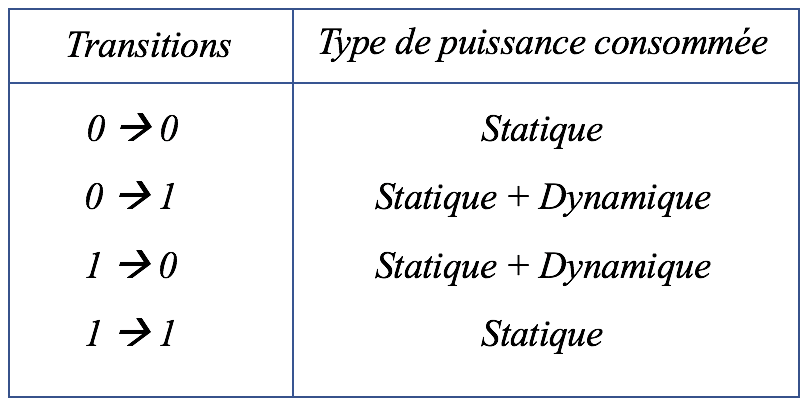
\includegraphics[scale=0.4]{image/dyn}
    \caption{Type de puissance consommée par une cellule CMOS en fonction des 4 transitions d'état de sa sortie.}
    \label{fig:dyn} 
\end{figure}

\hspace{-0.5 cm}On constate que pour chaque transition possible, il y a présence de puissance statique. Cependant, il n'y présence de puissance dynamique que dans le cas d'une commutation, c'est-à-dire dans les deux transitions suivantes : 0-1 et 1-0.  En toute logique, la consommation de puissance totale dépend du type de cellule et de la technologie employée. Cependant, en général, on constate que : 
\begin{itemize}
\item \textbf{\textit{Lorsqu'il n'y a pas de commutation}}(transitions 0-0 et 1-1), la puissance totale reste plus ou moins constante. En effet, la puissance dynamique étant nulle, on ne retrouve dans le calcul de puissance total que la puissance statique. Autrement dit : $P_{total}=P_{stat}$.
\item \textbf{\textit{Lorsqu'il y a une commutation}} (transitions 0-1 et 1-0), la puissance totale augmente. En effet, en plus de la puissance statique vient s'ajouter la puissance dynamique. Autrement dit : $P_{total}=P_{stat}+P_{dyn}$.
\end{itemize}

\vspace{+0.5 cm}\hspace{-0.5 cm}\fbox{
\begin{minipage}{\textwidth}
Ainsi, on peut conclure que la consommation de puissance dynamique des circuits CMOS correspond à la puissance qui est consommée par le circuit lorsqu'il y a une commutation dans la cellule. Cette puissance constitue un facteur dominant dans la consommation de puissance totale. Il est donc primordial de pouvoir la calculer.
\end{minipage}
}

Le calcul de la consommation de puissance dynamique se divise en deux parties. Pour mieux comprendre pourquoi, reprenons l'exemple de l'inverseur CMOS.

\begin{enumerate}
\vspace{-0.2 cm}\item \textbf{\textit{Puissance moyenne de chargement de la capacité}} : La figure \ref{fig:transitors} présente le schéma de l'inverseur CMOS lorsqu'il y a une commutation de sa sortie de l'état 0 à l'état 1 (partie gauche du shéma) et lorsqu'il y a une commutation de sa sortie de l'état 1 à l'état 0 (partie droite du schéma). Pour rappel, le fonctionnement de l'inverseur est le suivant : Lorsque le signal d'entrée est à 1 (ou 0), la transistor du dessous est passant (ou bloqué) alors que celui du haut est bloqué (ou passant), la sortie est donc à 0 (ou 1). Maintenant, il faut regarder dans le cas d'une commutation à la sortie de l'inverseur CMOS. Si il y a une commutation de l'état 0 à l'état 1 en sortie, l'inverseur dessine un courant provenant de l'alimentation ($V_{DD}$) et venant charger le condensateur $C_L$. Ce courant est appelé \textit{courant de charge}. À contrario, lors d'une commutation de l'état 1 à l'état 0, l'inverseur décharge le courant du condensateur $C_L$ vers la masse ($GND$). Ainsi, on constate bien que la commutation à la sortie de l'inverseur génère un courant qui produira une partie de la consommation de puissance dynamique. La consommation de puissance moyenne de chargement de la capacité durant un temps T peut être calculé de la façon suivante (\ref{eqn:charge}) :
\begin{gather}
	P_{chrg} = \frac{1}{T}\int_{0}^{T}p_{chrg}(t)dt=\alpha.f.C_{L}.V_{DD}^{2}\label{eqn:charge}
\end{gather}
Où : 
\begin{itemize}
\item $p_{chrg}(t)$ représente la consommation de puissance de chargement instantané de la cellule.
\item $\alpha$ est le facteur d'activité. Il correspond au nombre moyen de transitions (0-1) en sortie de la cellule à chaque coup de clock.
\item $f$ représente la fréquence de clock.
\item $C_L$ représente la valeur de capacité du condensateur.
\item $V_{DD}$ représente la tension positive de l'alimentation. \\
\end{itemize}


\vspace{-0.2 cm}\item \textbf{\textit{Puissance moyenne causée par les courants de court-circuit}} : En plus de la puissance moyenne de chargement de la capacité, il existe lors d'une commutation un bref instant, durant lequel les deux transistors conduisent le courant. Cela a pour effet de créer un court-circuit entre $V_{DD}$ en $GND$. Ce court-circuit va dissiper, le temps de son passage, de la puissance. La consommation de puissance moyenne qui est causée par les courants de court-circuit dans une cellule durant un temps T peut être calculé de la façon suivante (\ref{eqn:charge}) :
\begin{gather}
	P_{cc} = \frac{1}{T}\int_{0}^{T}p_{cc}(t)dt=\alpha.f.C_{L}.V_{DD}.I_{fuite}.t_{cc}
\end{gather}

Où : 
\begin{itemize}
\item $p_{cc}(t)$ représente la puissance de court-circuit consommée par la cellule.
\item $\alpha$ est le facteur d'activité. Il correspond au nombre moyen de transitions (0-1) en sortie de la cellule à chaque coup de clock.
\item $f$ représente la fréquence de clock.
\item $V_{DD}$ représente la tension positive de l'alimentation.
\item $I_{fuite}$ représente le courant de fuite causé par le court-circuit.
\item $t_{cc}$ représente le temps durant lequel le court-circuit existe.
\end{itemize}

\end{enumerate}



\subsubsection{Composition des traces de puissance}
Les attaques basées sur l'analyse de la consommation de puissance exploitent le fait que la consommation de puissance d'un device cryptographique dépend des \textbf{opérations qu'il exécute} et des \textbf{données qu'il manipule}. Ces deux informations vont ainsi permettre de définir différentes propriétés intéressantes. Pour chaque point analysé dans une trace de puissance, on notera :
\begin{itemize}
\item \textbf{$P_{op}$ la composante dépendante de l'opération exécutée} ;
\item \textbf{$P_{data}$ la composante dépendante de la donnée manipulée}. \\
\end{itemize}
De plus, une troisième composante doit également être prise en compte. Cette composante fait référence au \textbf{bruit électrique} (aussi appelé bruit de fond) et sera notée \textbf{$P_{noise}$}. En effet, un signal est toujours affecté de petites fluctuations plus ou moins importantes. Ces fluctuations, dont les origines peuvent être diverses, sont appelées bruit électrique (ou simplement bruit). Le bruit est considéré comme un élément parasite aléatoire, c'est-à-dire qu'on ne sait pas le déterminer à l'avance. Au plus cette composante sera élevée et au plus l'analyse de la consommation de puissance sera difficile.

Ainsi, chaque point d'une trace de puissance peut être modélisé comme la somme des 3 composantes définies ci-dessus, soit : 
$P_{total} = P_{op} + P_{data} + P_{noise}$.

\subsubsection{Modèles de puissance}

Distance de Hamming...

Poids de Hamming ...

\subsubsection{L'attaque CPA en concret}

La figure \ref{fig:CPAconcrete} ci-dessous présente le principe de fonctionnement d'une attaque CPA comme décrite ci-avant.

\newpage

\subsection{Simulations sur MATLAB}

Afin de bien assimiler une attaque par canal auxiliaire, il m'a été demandé de tester, par des simulation sur le logiciel MATLAB, les notions théoriques développées précédemment. Deux exercices différents ont ainsi été réalisés. 
\begin{enumerate}
\item \textbf{Simuler un point d'une trace et ensuite réaliser une attaque CPA sur ce point}. La première phase de la simulation a pour objectif de génèrer un point particulier d'une trace sur base de l'algorithme AES. La seconde phase de la simulation a pour but de réaliser une attaque par canal auxiliaire. Plus précisément, il s'agit d'une attaque CPA. Pour cette raison, seules les 2 premières étapes de l'algorithme AES sont nécessaires et seront donc simulées (\textit{AddRoundKey}, \textit{SubBytes}). À noter que, pour simplifier, cette attaque n'est réalisée que sur un seul byte de données et donc aussi un seul byte de clé.
\item \textbf{Réaliser une attaque CPA à partir de traces réelles}. Dans ce cas de figure, on connait 4 paramètres : les messages clairs envoyés (plaintexts), les traces capturées à l'oscilloscope, le nombre de traces ainsi que le nombre d'échantillons. Ainsi, sur base des traces qui nous sont fournies, l'objectif est de tenter de retrouver la clé secrète en réalisant une attaque CPA. La différence majeure avec l'exercice précédent est que l'on étudie une trace selon l'ensemble de points (les échantillons) qui la caractérise. Cet ensemble de traces étant par ailleurs fournit sur base de mesures réalisées à l'oscilloscope. \\
\end{enumerate}

\hspace{-0.5 cm}\textbf{\underline{Exercice 1 :}} La figure \ref{fig:simul1} ci-dessous représente le schéma-bloc de la première phase de l'exercice 1, c'est-à-dire qu'il présente les différentes étapes à réaliser pour simuler un point d'une trace.
\begin{figure}[htbp]
    \centering
    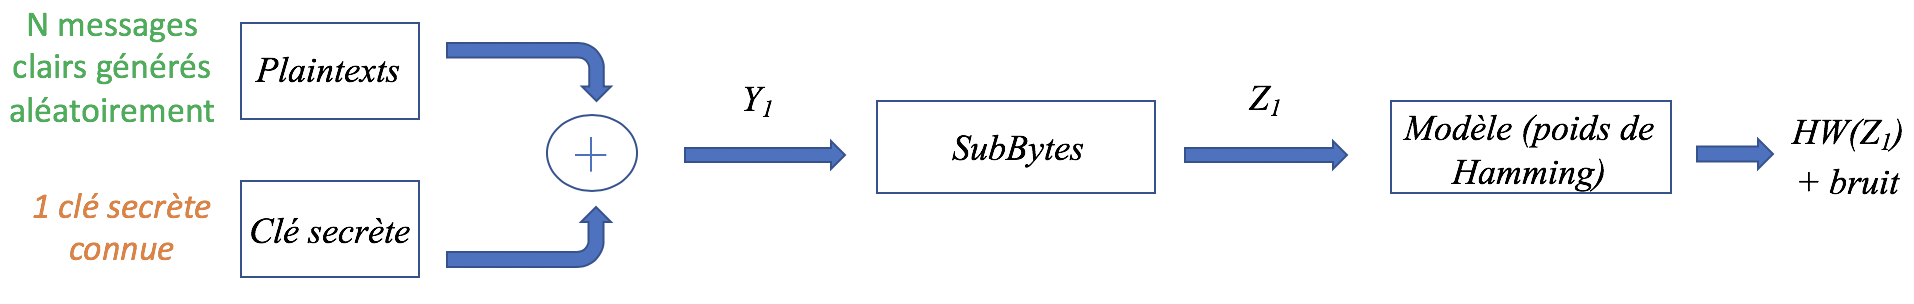
\includegraphics[scale=0.45]{image/simul1}
    \caption{Schéma-bloc permettant de comprendre la simulation d'un point d'une trace.}
    \label{fig:simul1} 
\end{figure}

\vspace{-0.4 cm}Sur le schéma-bloc, nous percevons deux entrées : la clé secrète (connue) utilisée pour le chiffrement ainsi que les N messages clairs devant être chiffrés. Nous réalisons ensuite les deux premières étapes de l'algorithme AES, à savoir les opérations \textit{AddRoundKey} (correspondant à un \textit{XOR}) et \textit{SubBytes} respectivement. Le résultat obtenu à la sortie de l'opération \textit{AddRoundKey} est noté \textit{$Y_1$} alors que celui obtenu à la sortie de l'opération \textit{SubBytes} est noté \textit{$Z_1$}. Ensuite, un modèle de puissance est utilisé afin d'imiter au mieux la consommation de puissance du circuit. Ce modèle de puissance est le \textit{poids de Hamming}. Le but est donc de compter le nombre de bits à '1' pour chaque octet de données \textit{$Z_1$}. Le résultat obtenu est noté \textit{$HW(Z_1)$}. Enfin, une fois que le poids de Hamming a été calculé, on ajoute du bruit afin de rendre la simulation plus réelle. En effet, en réalité, lors d'une prise de mesure, un élément parasite vient toujours s'additionner au signal que l'on étudie, il s'agit de bruit électronique.

La figure \ref{fig:simul2} ci-dessous représente le schéma-bloc de la seconde phase de l'exercice 1. Il présente ainsi les différentes étapes à réaliser qui serviront \textit{in fine} à réaliser l'attaque CPA.
\begin{figure}[htbp]
    \centering
    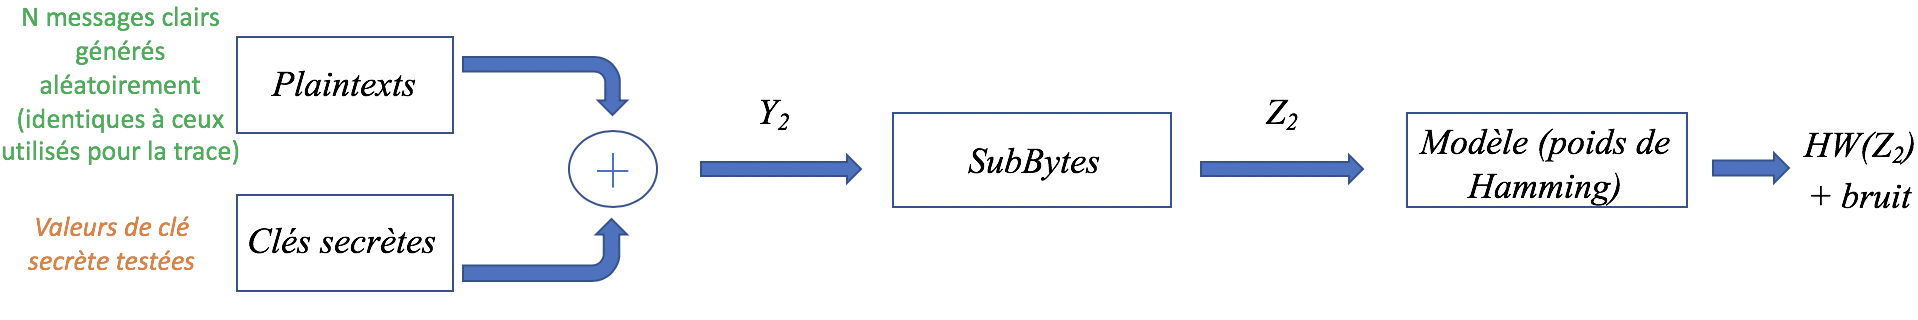
\includegraphics[scale=0.45]{image/simul2}
    \caption{Schéma-bloc permettant de comprendre la seconde phase de l'exercice 1.}
    \label{fig:simul2} 
\end{figure}

\vspace{-0.4 cm}La figure \ref{fig:simul2} est quasi identique à la figure \ref{fig:simul1}. La seule différence concerne l'une des deux entrées. En effet, le but de l'attaque CPA est de retrouver la clé secrète utilisée dans la figure \ref{fig:simul1} pour chiffrer nos N messages. Ainsi, si on ne s'intéresse qu'à un seul octet de données et donc, par la même occasion, à un seul octet de clé, on va tester les 256 ($2^8$) valeurs de clé possibles. En notant respectivement $Y_2$ et $Z_2$ les résultats obtenus en sortie des opérations \textit{AddRoundKey} et \textit{SubBytes}, il ne nous restera plus qu'à calculer le poids de Hamming et à ajouter du bruit pour ensuite tenter de retrouver la clé secrète par calcul du coefficient de corrélation.


Concrètement, sur MATLAB, tous ces calculs vont être opérés sur des matrices. La figure \ref{fig:simulCPA1} présente les différentes tailles de matrices utilisées pour réaliser la simulation.
\begin{figure}[htbp]
    \centering
    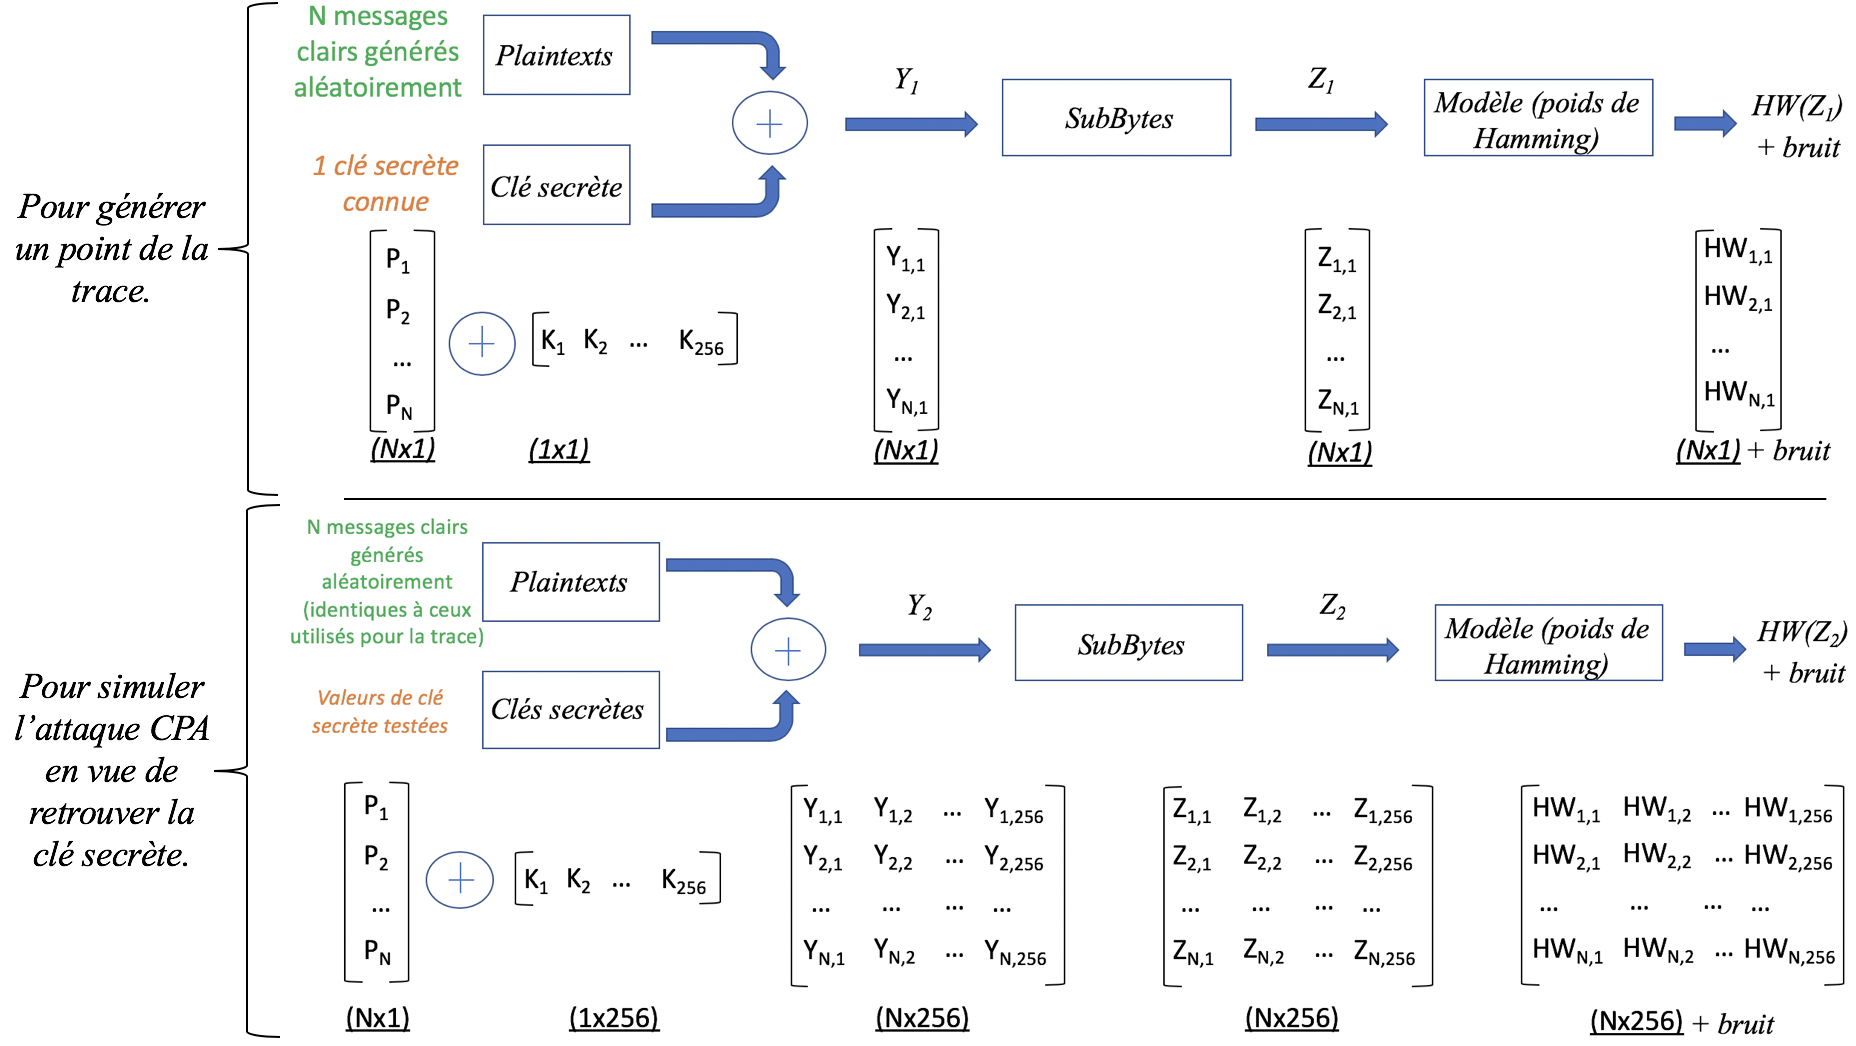
\includegraphics[width=0.9\textwidth]{image/simulCPA1}
    \caption{Schéma-bloc permettant de visualiser la taille des différentes matrices employées pour la simulation.}
    \label{fig:simulCPA1} 
\end{figure}

\vspace{-0.3 cm}Comme vu à la section \ref{sec:AES}, l'algorithme AES implémente deux matrices en entrée : la matrice STATE et la matrice clé. Ces deux matrices contiennent 16 éléments correspondants aux 16 octet de données (pour la matrice STATE) et aux 16 octets de clé (pour la matrice clé). Autrement dit, ces deux matrices sont de tailler 4x4. Pour le test, nous allons simplifier le procédé. En effet, en pratique les opérations s'exécutent octect par octet. Dans notre cas, on ne va s'intéresser qu'au premier octet de la matrice STATE et donc, par la même occasion, au premier octet de la matrice clé. \textbf{\textit{Le but final de la simulation sera donc de retrouver le premier octet de la clé connaissant le premier octet des N messages clairs devant être chiffrés.}}
Ainsi :
\begin{itemize}
\item La matrice STATE est représentée par une matrice de taille Nx1. N représente le nombre de messages clairs envoyés.
\item La matrice clé, dans le cas de la génération d'un point de la trace, est représentée par une matrice de taille 1x1. Un seul octet de l'unique clé secrète est en effet utilisé.
\item La matrice clé, dans le cas de la simulation par ordinateur, est représentée par une matrice de taille 1x256. En effet, le but étant de retrouver la valeur du premier octet de la clé secrète, il existe $2^8$ soit 256 valeurs possibles.
\item $Y_1$ et $Y_2$ sont des matrices de taille Nx1 etNx256 respectivement. En effet, pour $Y_1$, une seul clé est utilisée alors que pour $Y_2$, 256 valeurs de clé sont utilisées.
\item $Z_1$ et $Z_2$ sont des matrices de taille Nx1 et Nx256 respectivement. En effet, l'opération \textit{SubBytes} ne modifie pas la taille des données obtenues précédemment ($Y_1$ et $Y_2$).
\item Enfin, $HW(Z_1)$ et $HW(Z_2)$ sont des matrices de taille Nx1 et Nx256 pour les mêmes raisons évoquées précédemment. \\
\end{itemize}

\vspace{-0.2 cm}Pour rappel, le but final de la simulation est de retrouver le premier octet de la clé connaissant un point de la trace (obtenu par simulation) et connaissant les N messages clairs envoyés. Cela sera rendu possible en calculant le coefficient de corrélation pour chaque valeur de clé possible. Le figure \ref{fig:CorrEx1} ci-dessous présente le calcul final qui permettra de retrouver le premier octet de la clé secrète.

\begin{figure}[htbp]
    \centering
    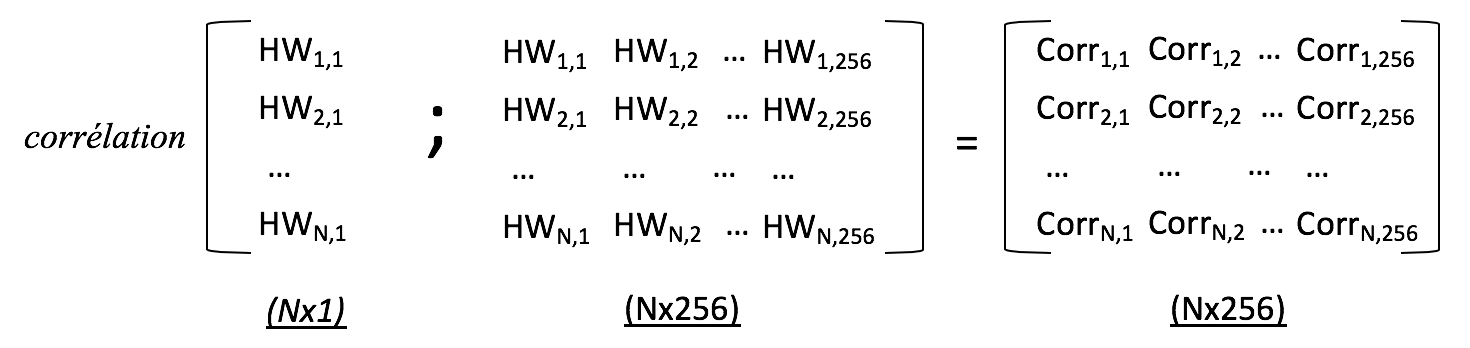
\includegraphics[scale=0.35]{image/CorrEx1}
    \caption{Calcul du coefficient de corrélation entre un point d'une trace simulée et le poids de Hamming.}
    \label{fig:CorrEx1} 
\end{figure}

\newpage
Les graphes \ref{fig:10}, \ref{fig:100} et \ref{fig:1000} ci-dessous présentent les résultats obtenus. Il s'agit de graphes indiquant les valeurs de coefficient de corrélation en fonction des 256 valeurs de clé testées. En toute logique, le coefficient de corrélation est maximum (en valeur absolue) pour la clé réellement utilisée pour le chiffrement des données. Cependant, on sait qu'en fonction du nombres de traces analysées, les valeurs du facteur de corrélation fluctuent dans un intervalle plus ou moins grand. Ainsi, au plus le nombre de traces sera grand, au plus l'intervalle des valeurs de corrélation sera petit et au plus ce sera facile de repérer la clé de chiffrement. En effet, si on observe les trois graphes ci-dessous, on peut remarquer que pour 10 traces, le coefficient de corrélation varie entre -0,83 et 0,8 ; pour 100 traces, le coefficient de corrélation varie entre -0,26 et 0,34 ; pour 1000 traces, le coefficient de corrélation varie entre -0,24 et 0,21. Pour chacun des trois graphes, on peut néanmoins distinguer la valeur de la clé secrète dont la valeur du coefficient de corrélation culmine à 0,98. Dans l'exemple, la clé secrète qui était utilisée valait 200 (en décimal).

\begin{figure}[htbp]
    \centering
    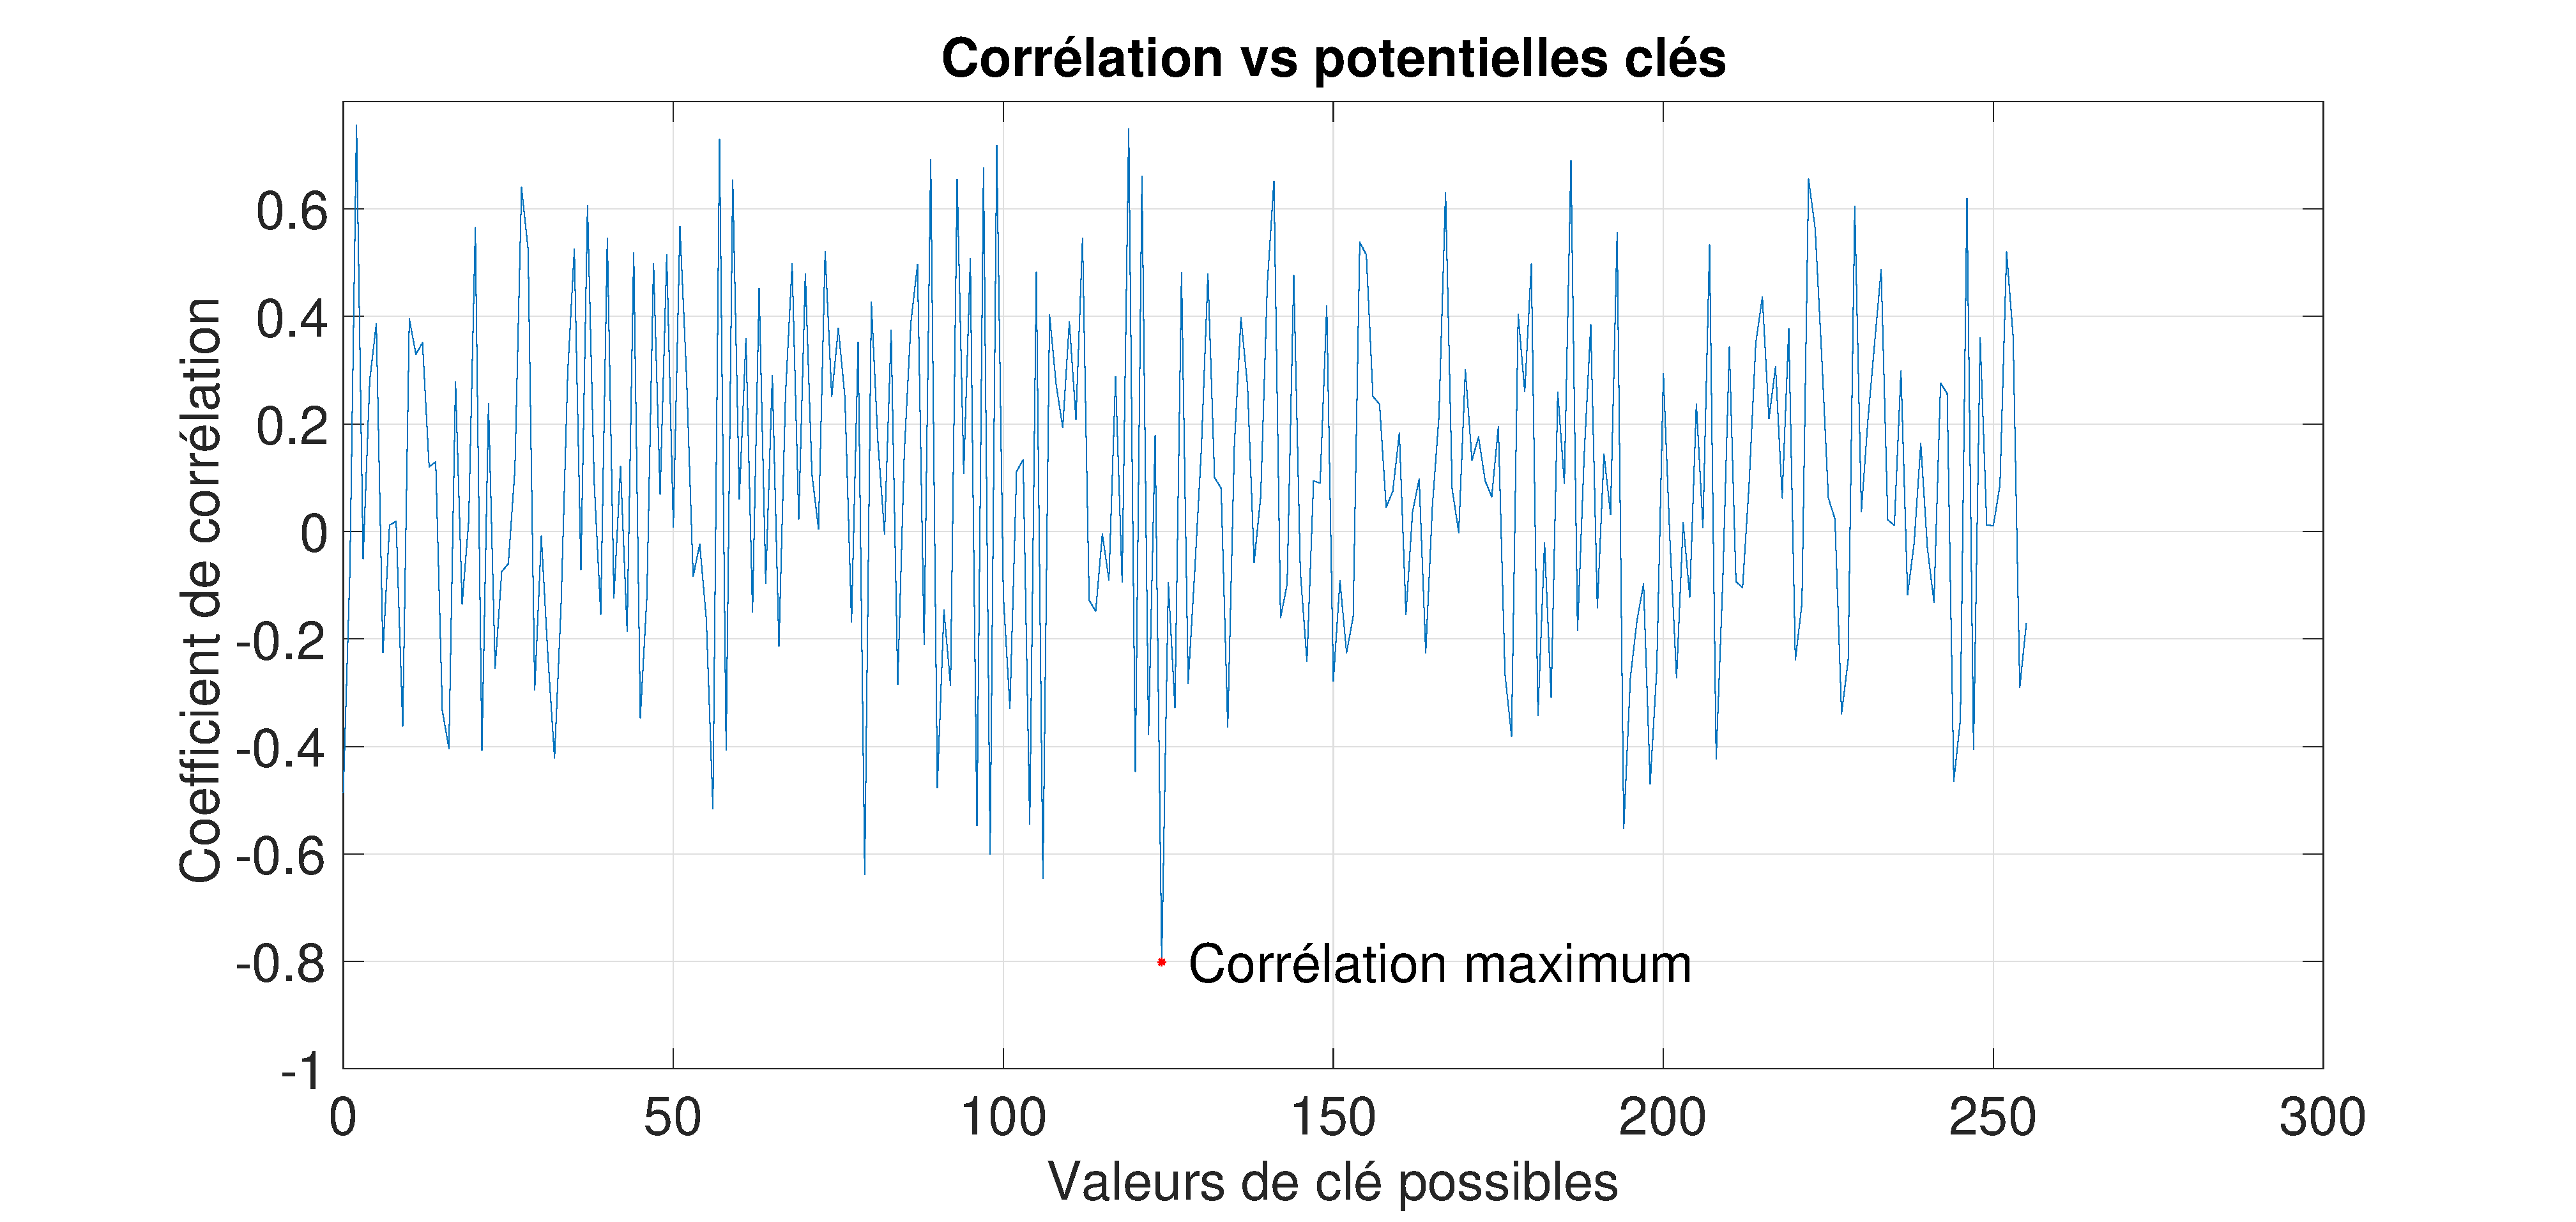
\includegraphics[width=0.95\textwidth]{image/10}    \caption{Coefficient de corrélation en fonction de la valeur de la clé lorsqu'on analyse 10 traces.}    \label{fig:10}
\end{figure}

\begin{figure}[htbp]
    \centering
    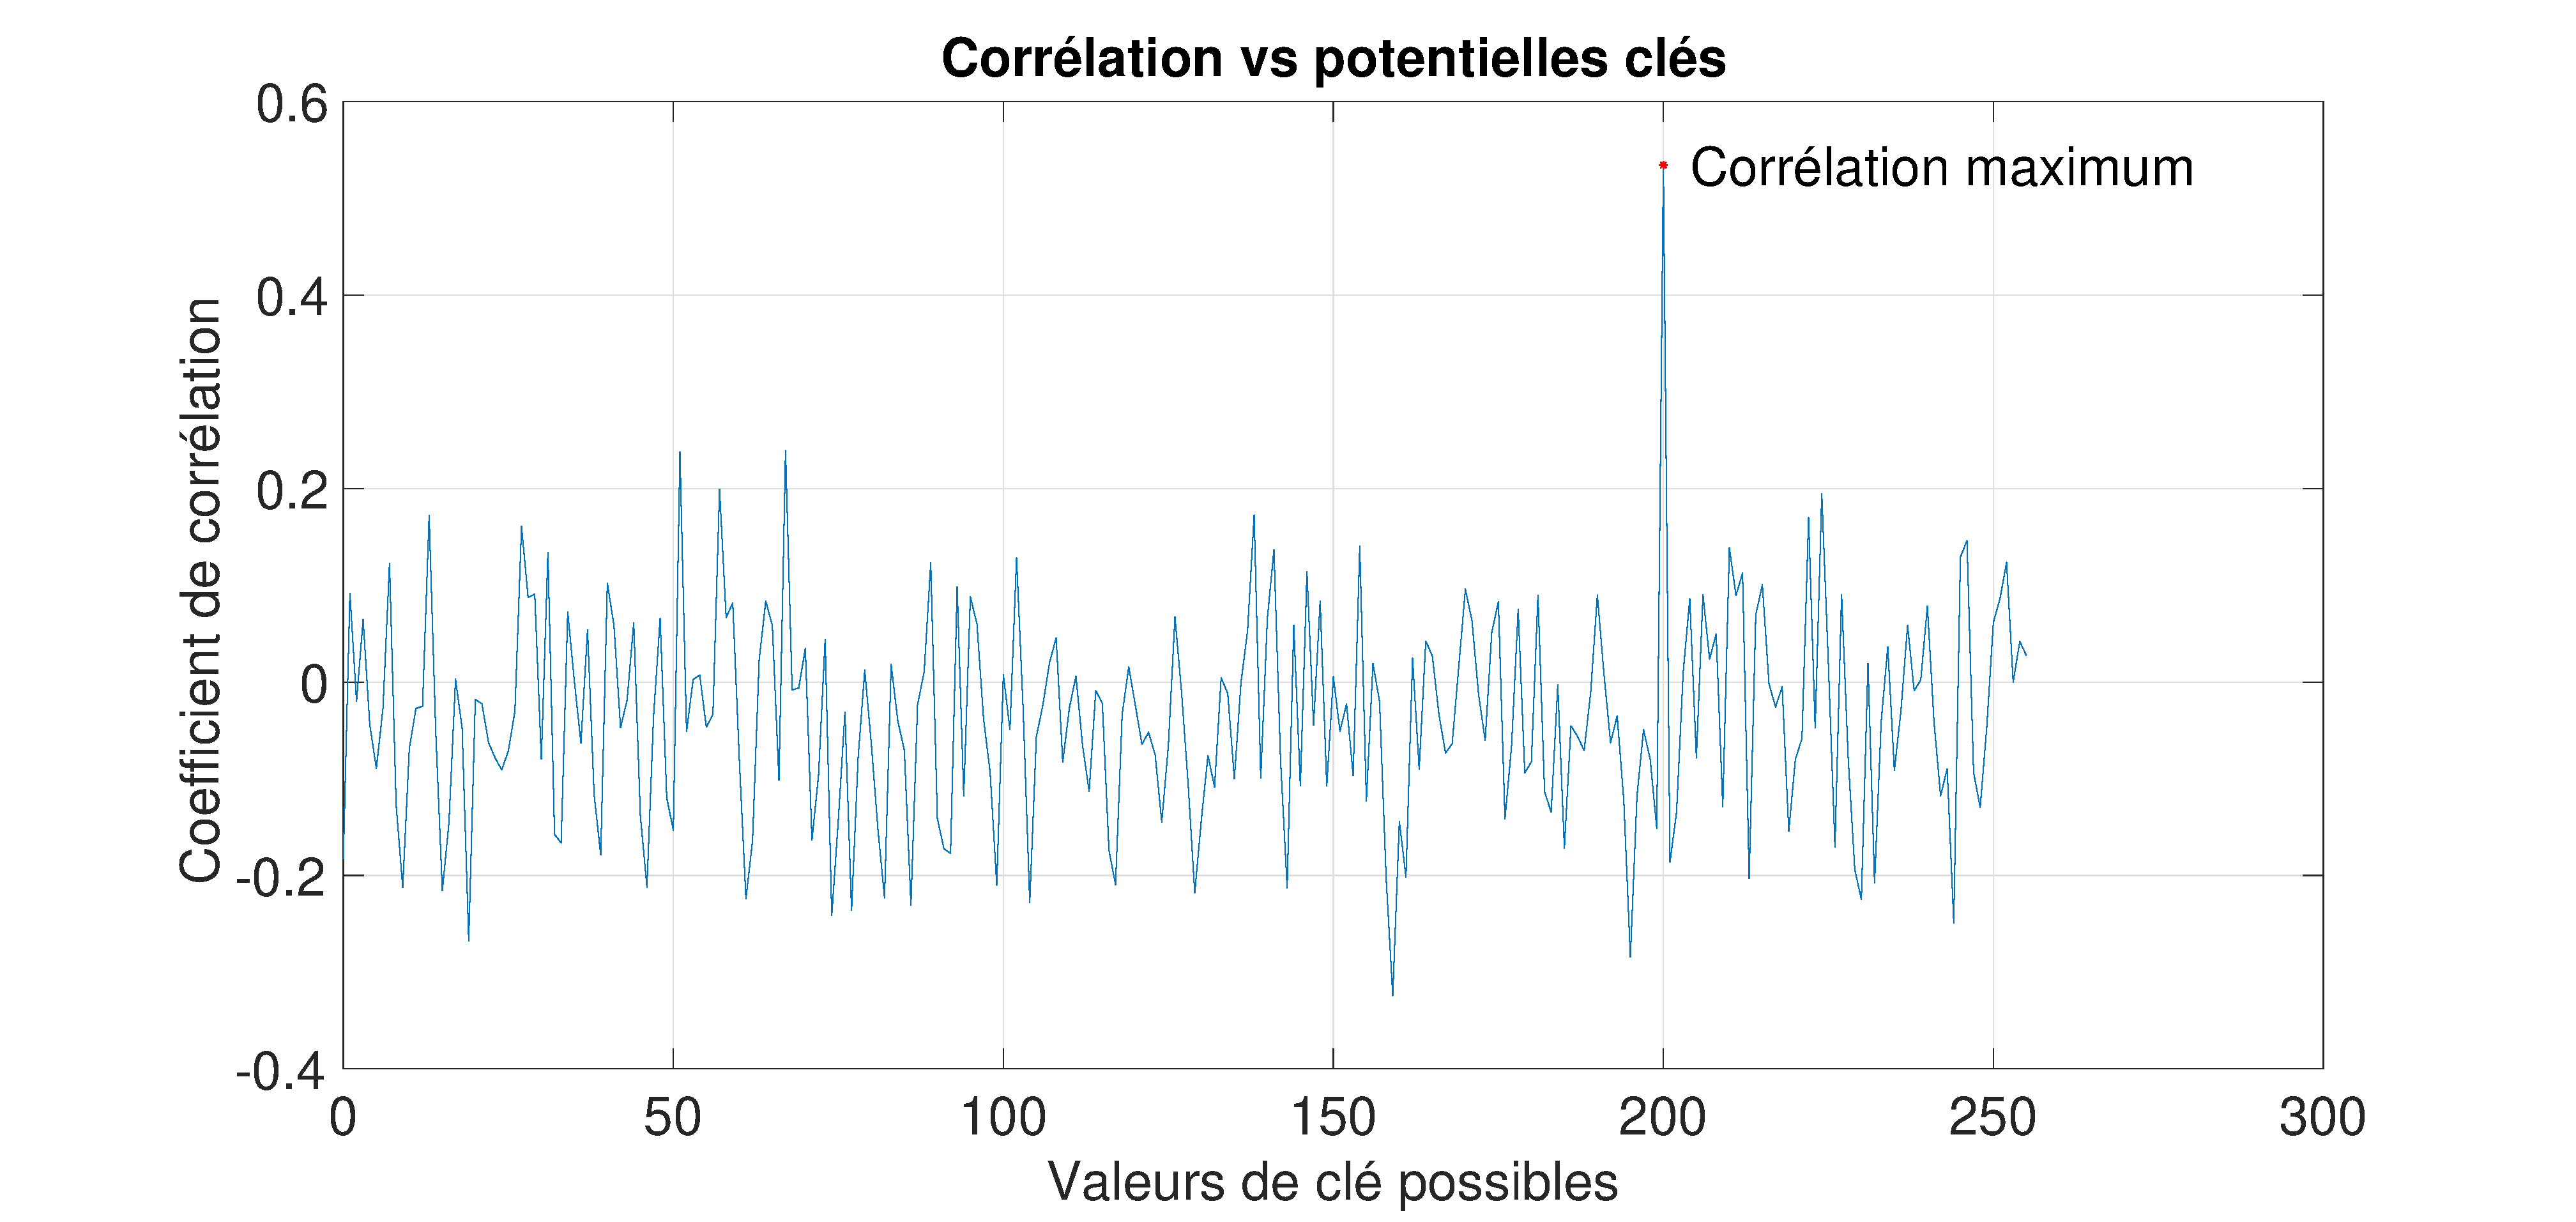
\includegraphics[width=0.95\textwidth]{image/100}    \caption{Coefficient de corrélation en fonction de la valeur de la clé lorsqu'on analyse 100 traces.}    \label{fig:100}
\end{figure}

\begin{figure}[htbp]
    \centering
    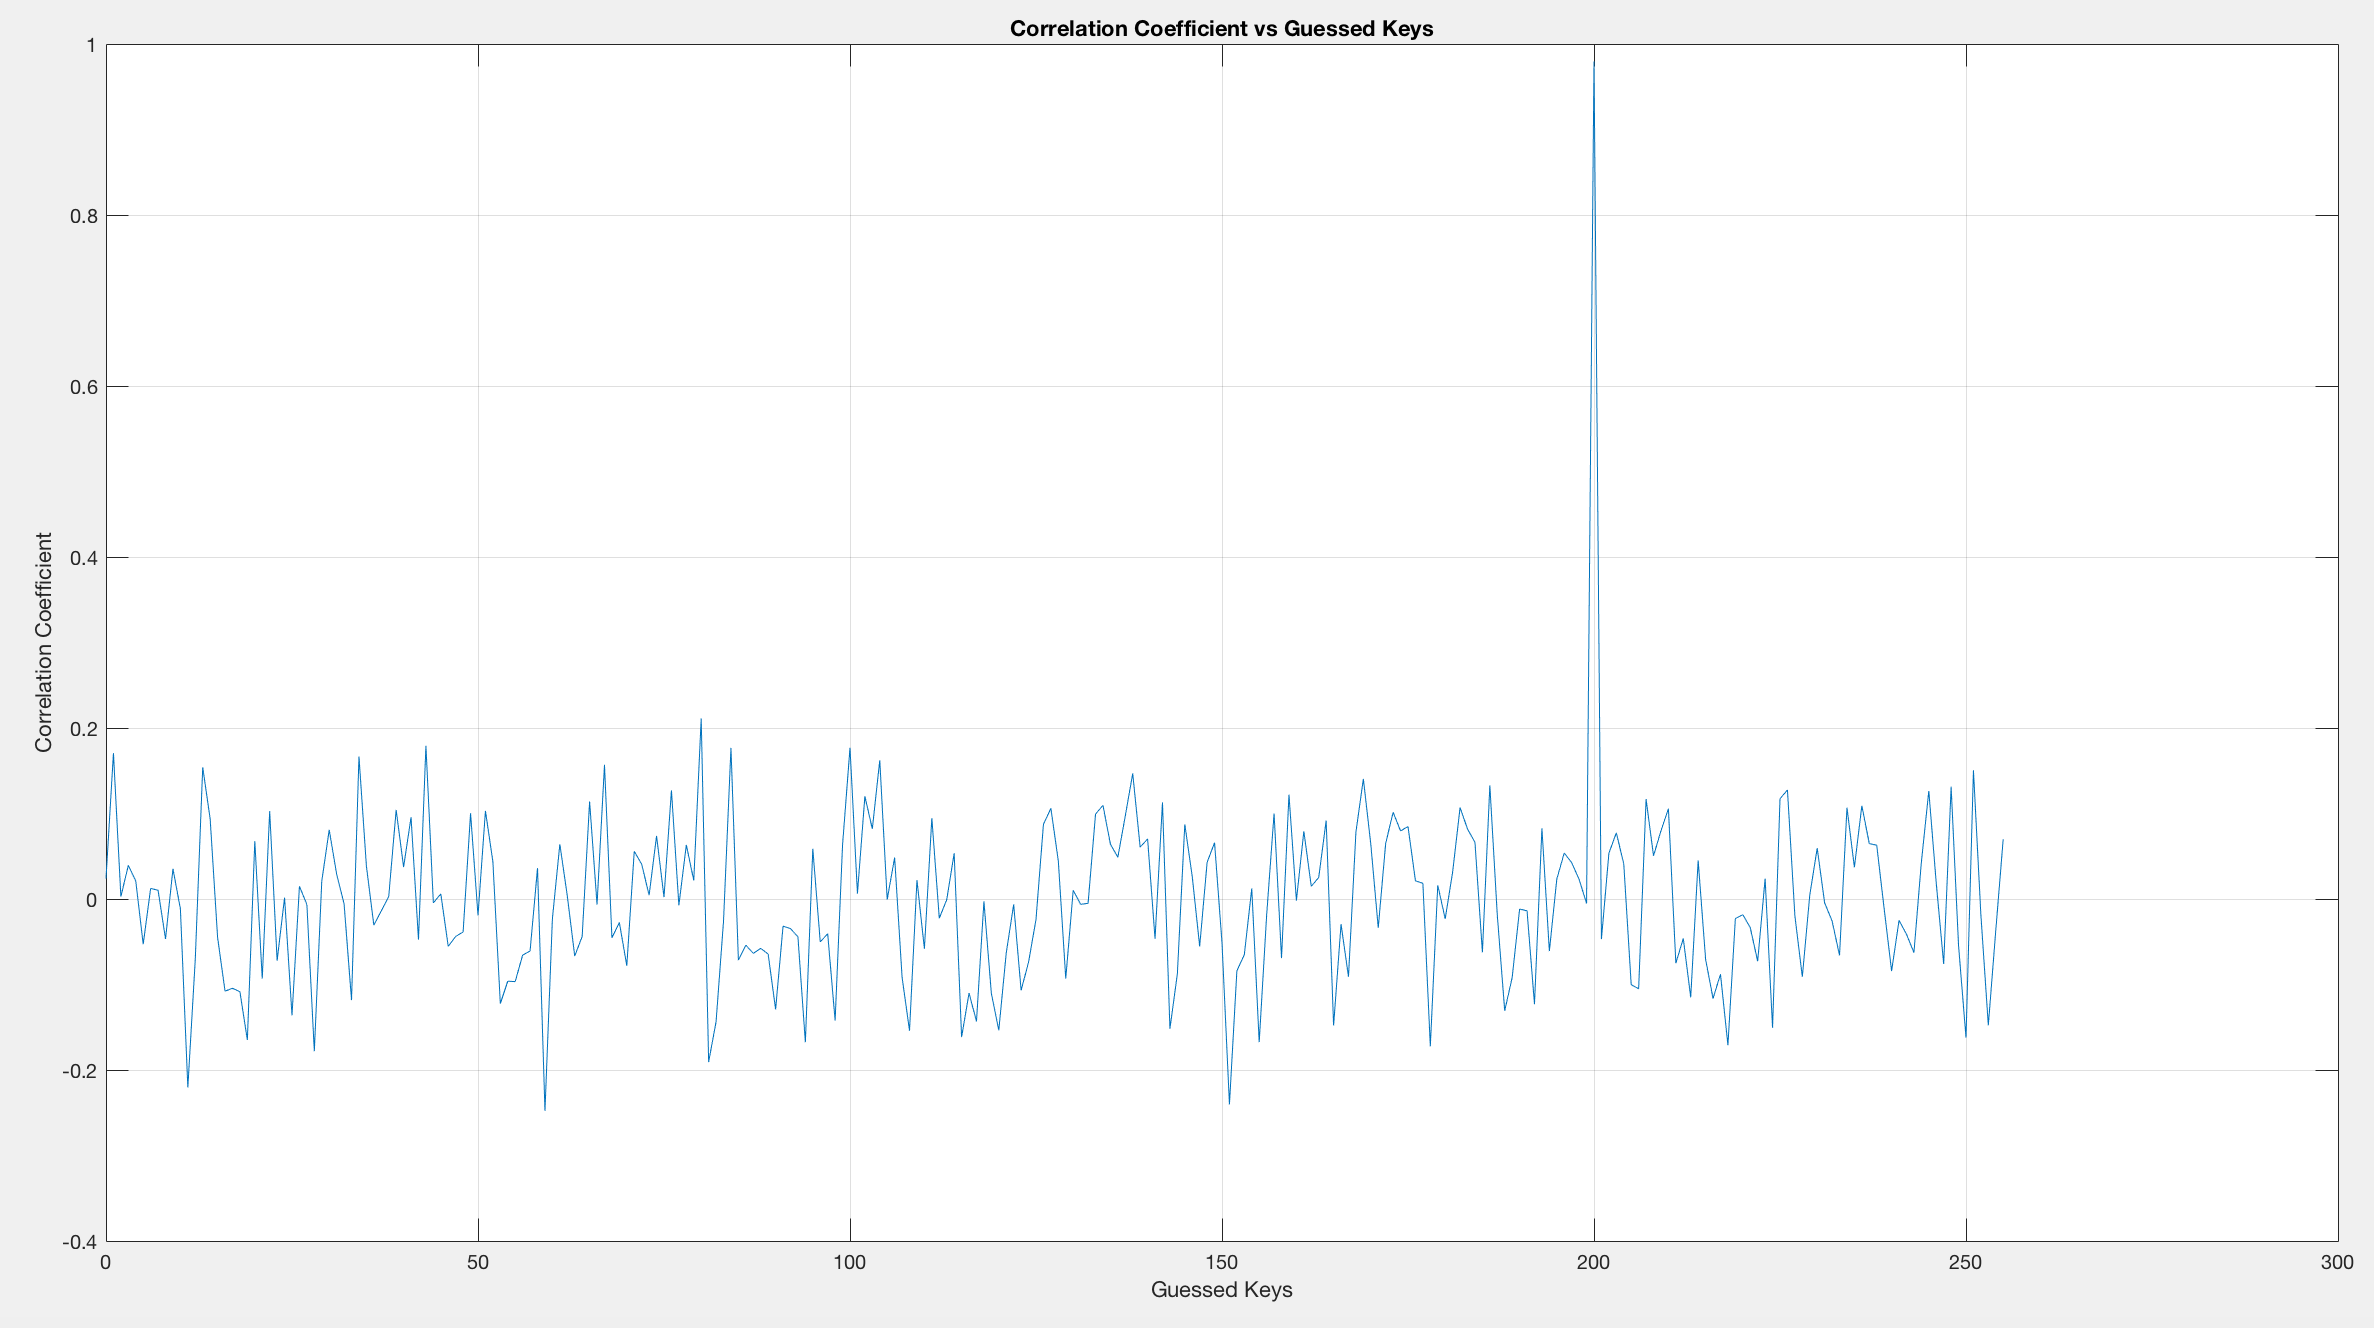
\includegraphics[width=1.05\textwidth]{image/1000}    \caption{Coefficient de corrélation en fonction de la valeur de la clé lorsqu'on analyse 1000 traces.}    \label{fig:1000}
\end{figure}

\newpage

\hspace{-0.5 cm}\textbf{\underline{Exercice 2 :}} La figure \ref{fig:simulEx2} ci-dessous représente le schéma-bloc de l'exercice 2. Dans cet exercice, on confronte les mesures obtenues à l'oscilloscope avec le poids de Hamming calculé à partir des messages clairs et pour chaque valeur de clé. À noter que dans cet exercice, on opère toujours sur le premier octet de données et le premier octet de la clé.
\begin{figure}[htbp]
    \centering
    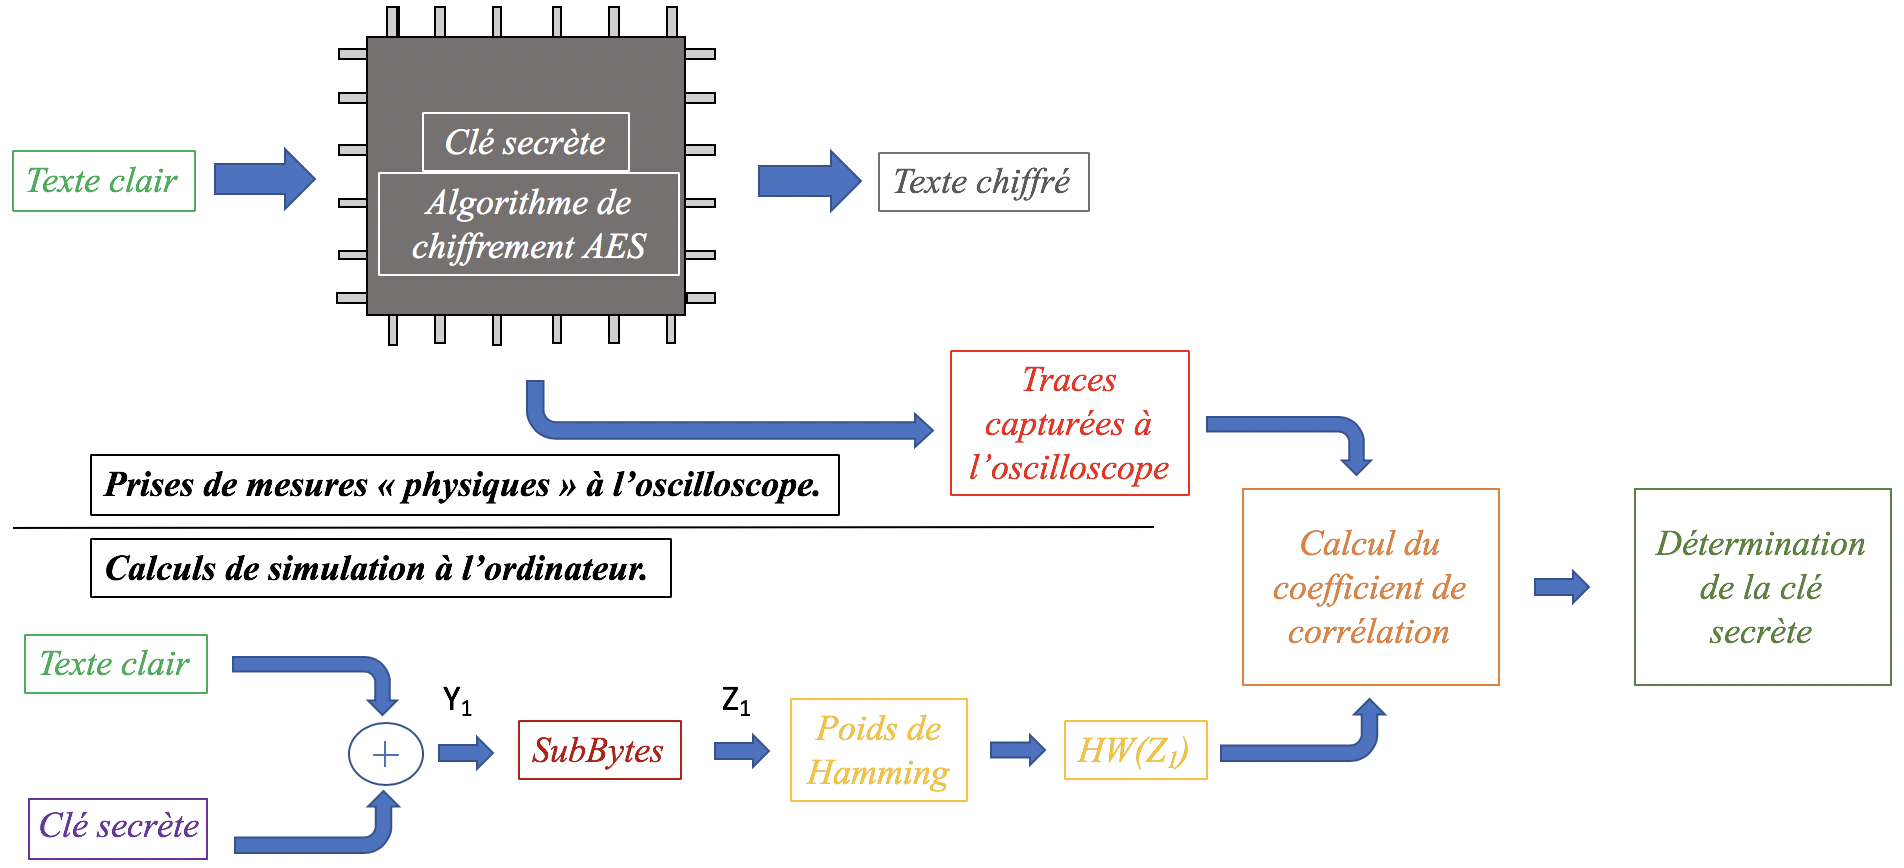
\includegraphics[scale=0.4]{image/simulEx2}
    \caption{Schéma-bloc permettant de comprendre le principe de fonctionnement du deuxième exercice.}
    \label{fig:simulEx2} 
\end{figure}

\vspace{-0.3 cm}On distingue 3 grands blocs sur le schéma ci-dessus :
\begin{itemize}
\item Premièrement, la prise de mesures à l'oscilloscope. Cette prise de mesure nous fournit un ensemble de traces. Plus précisément, l'oscilloscope a enregistré N traces différentes.
\item Deuxièmement, des calculs de simulation de la consommation de puissance à partir du modèle du \textit{poids de Hamming}. Pour chaque texte clair envoyé et pour chaque clé possible, on va calculer le poids de Hamming du résultat obtenu en sortie de l'opération \textit{SubBytes}. Ce bloc est identique à la figure \ref{fig:simul2}.
\item Dernièrement, le calcul du coefficient de corrélation. Cette corrélation est effectuée pour chaque trace capturée avec chaque résultat du poids de Hamming. 
\end{itemize}

\hspace{-0.5 cm}Voici les données dont nous disposons pour l'exercice :
\begin{itemize}
\item On connait le nombre de traces enregistrées à l'oscilloscope. Il y en a 2380.
\item On connait le nombre d'échantillons pris dans une seule trace. Il y en a 16384.
\item On connait tous les textes clairs envoyés au device cryptographique en vue d'être chiffrés. On a donc 2380 textes clairs connus. Chaque texte possédant une taille de 128 bits, soit 16 octets. Néanmoins, comme précisé précédemment, on ne s'intéresse qu'au premier octet.
\item On connait toutes les traces mesurées à l'oscilloscope. 2380 traces ont été enregistrées. Chaque trace contient 16384 points (échantillons). \\
\end{itemize}

\hspace{-0.5 cm}Les 4 figures suivantes permettent de mieux comprendre, en pratique, l'objectif de l'exercice :
\begin{enumerate}
\item La figure \ref{fig:traces} présente les quatre premières traces, parmi les 2380, mesurées à l'oscilloscope.
\item La figure \ref{fig:cle} présente les valeurs de coefficient de corrélation obtenues pour quatre clés possibles, à savoir les clés 128, 129, 130 et 131. Chaque valeur de corrélation est calculée pour chacun des 16384 points (échantillons) des 2380 traces. 
\item La figure \ref{fig:3D} présente en trois dimensions les valeurs de coefficient de corrélation obtenues pour les 256 valeurs de clé possibles. On remarque qu'il existe un coefficient de corrélation maximum, marqué par une étoile rouge sur la figure. Ce coefficient correspond à la clé 8 (en décimal). Cela signifie que le premier octet de la clé secrète vaut 8. 
\item La figure \ref{fig:cle8} présente les valeurs de coefficient de corrélation obtenues pour une valeur de clé correspondant à 8. Cette valeur présente le plus grand coefficient de corrélation et correspond donc au premier octet de la clé secrète. Le coefficient de corrélation maximum vaut effectivement 0,5099.
\end{enumerate}


\begin{figure}[htbp]
    \centering
    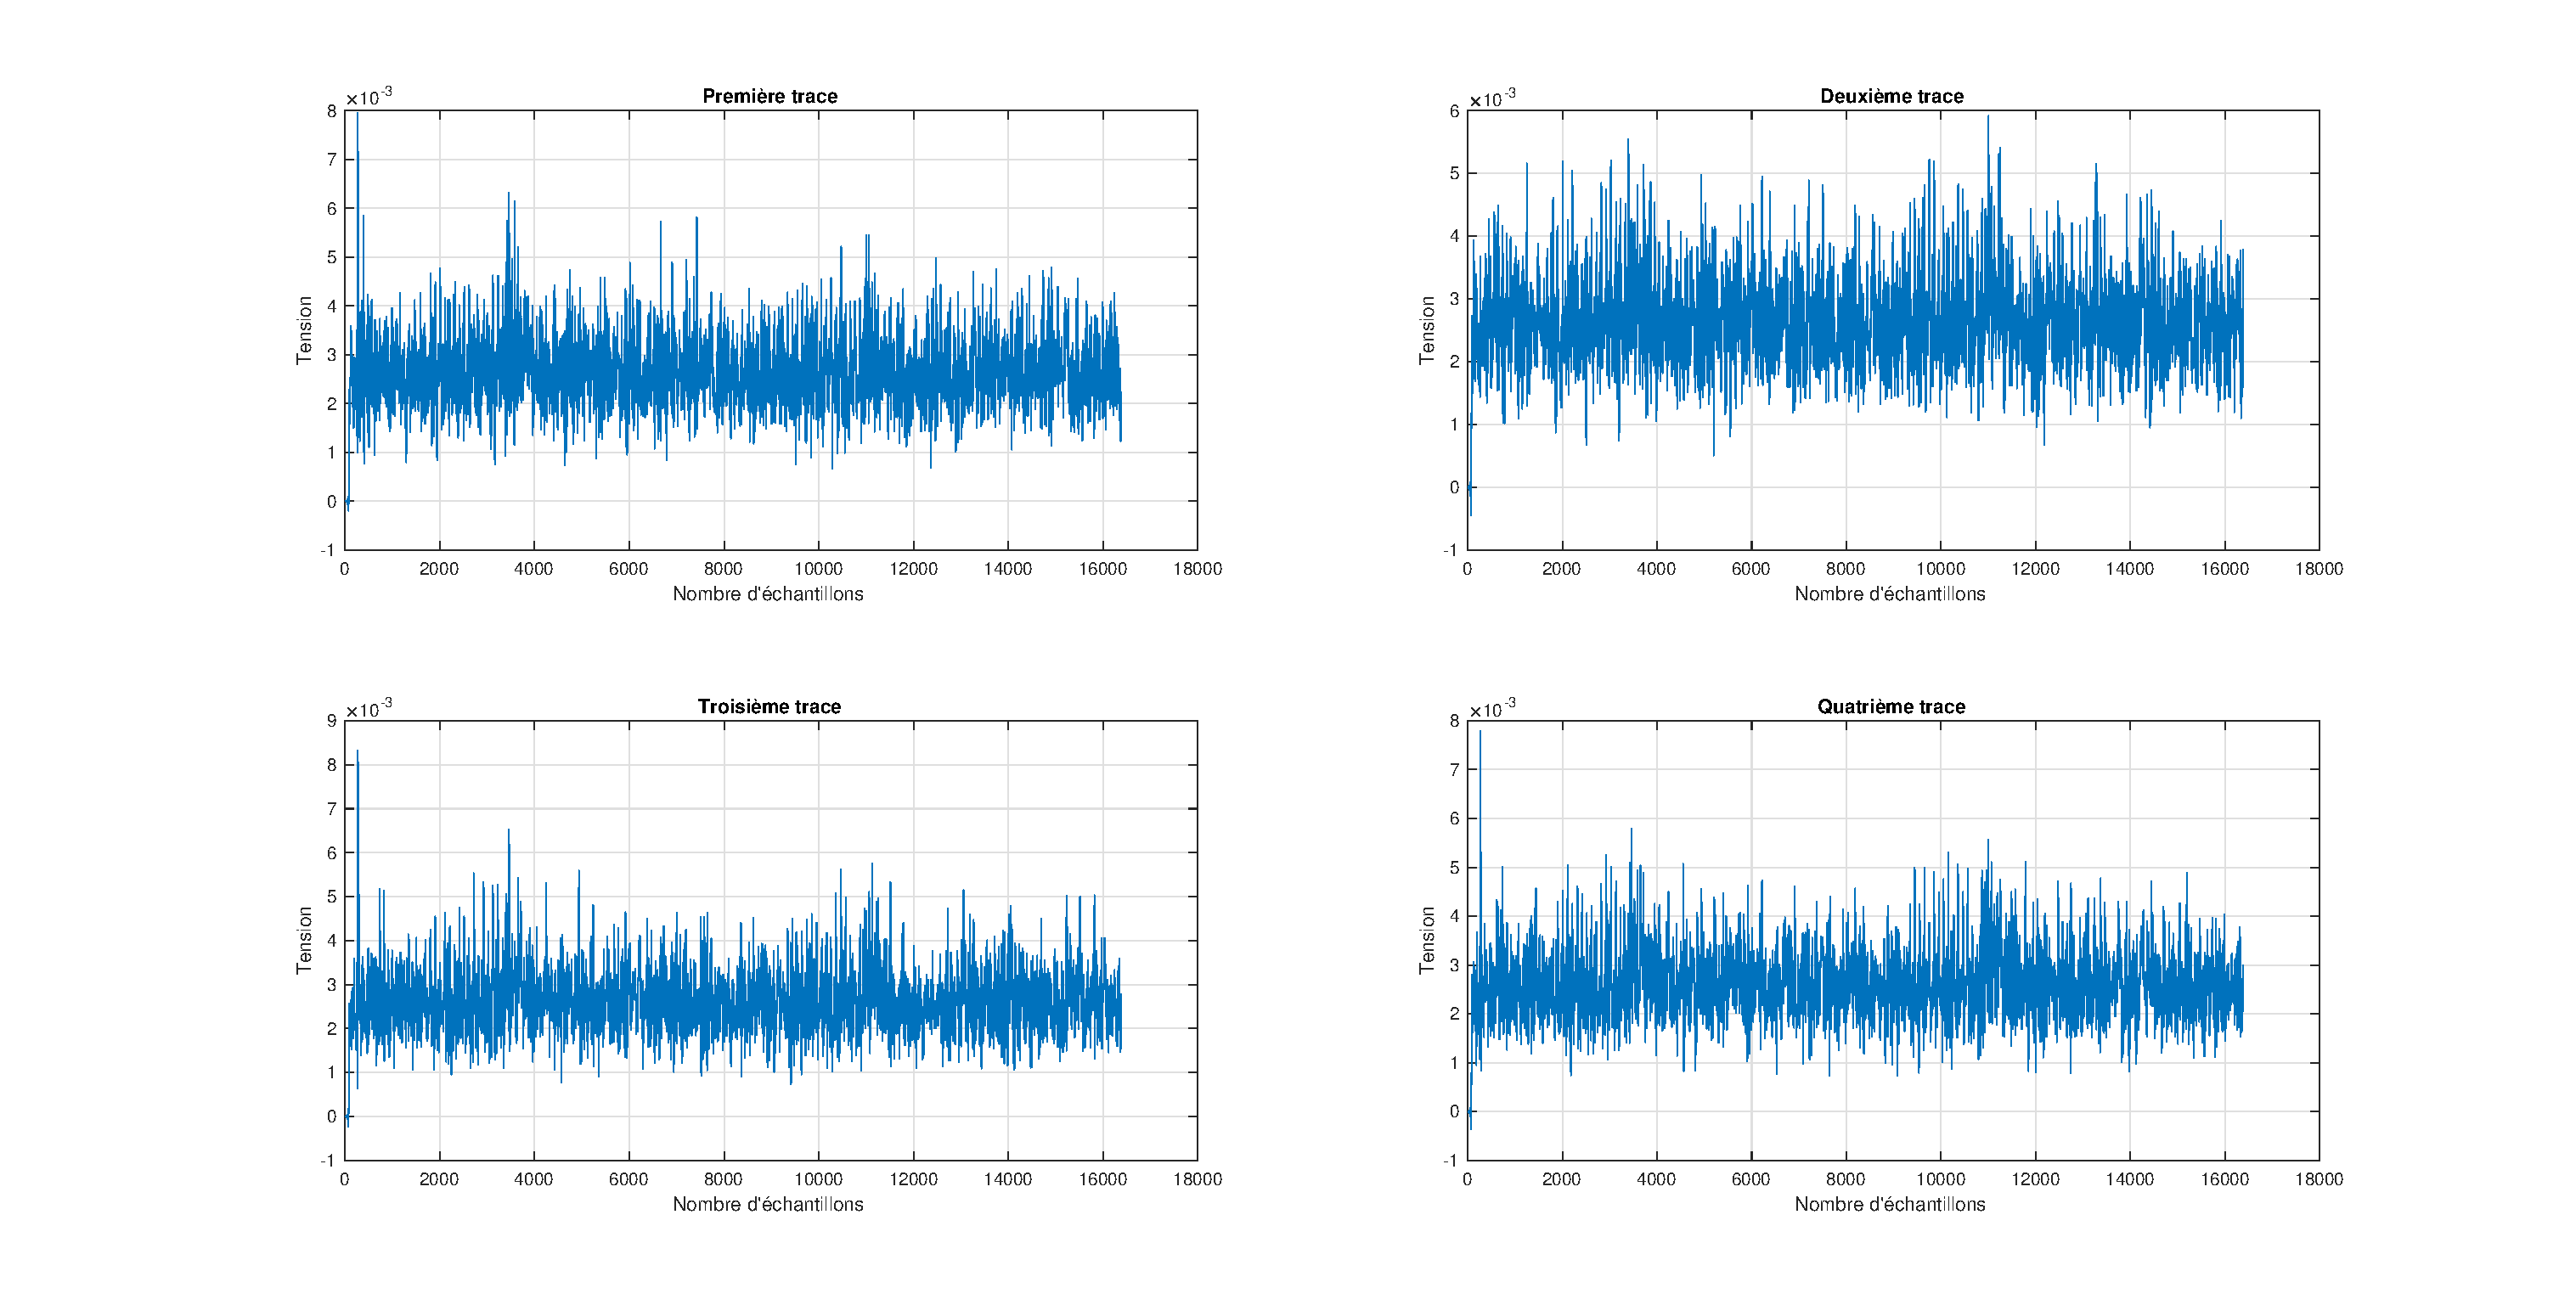
\includegraphics[scale=0.45, angle=90]{image/traces}
    \caption{Les 4 premières traces mesurées à l'oscilloscope.}
    \label{fig:traces} 
\end{figure}

\begin{figure}[htbp]
    \centering
    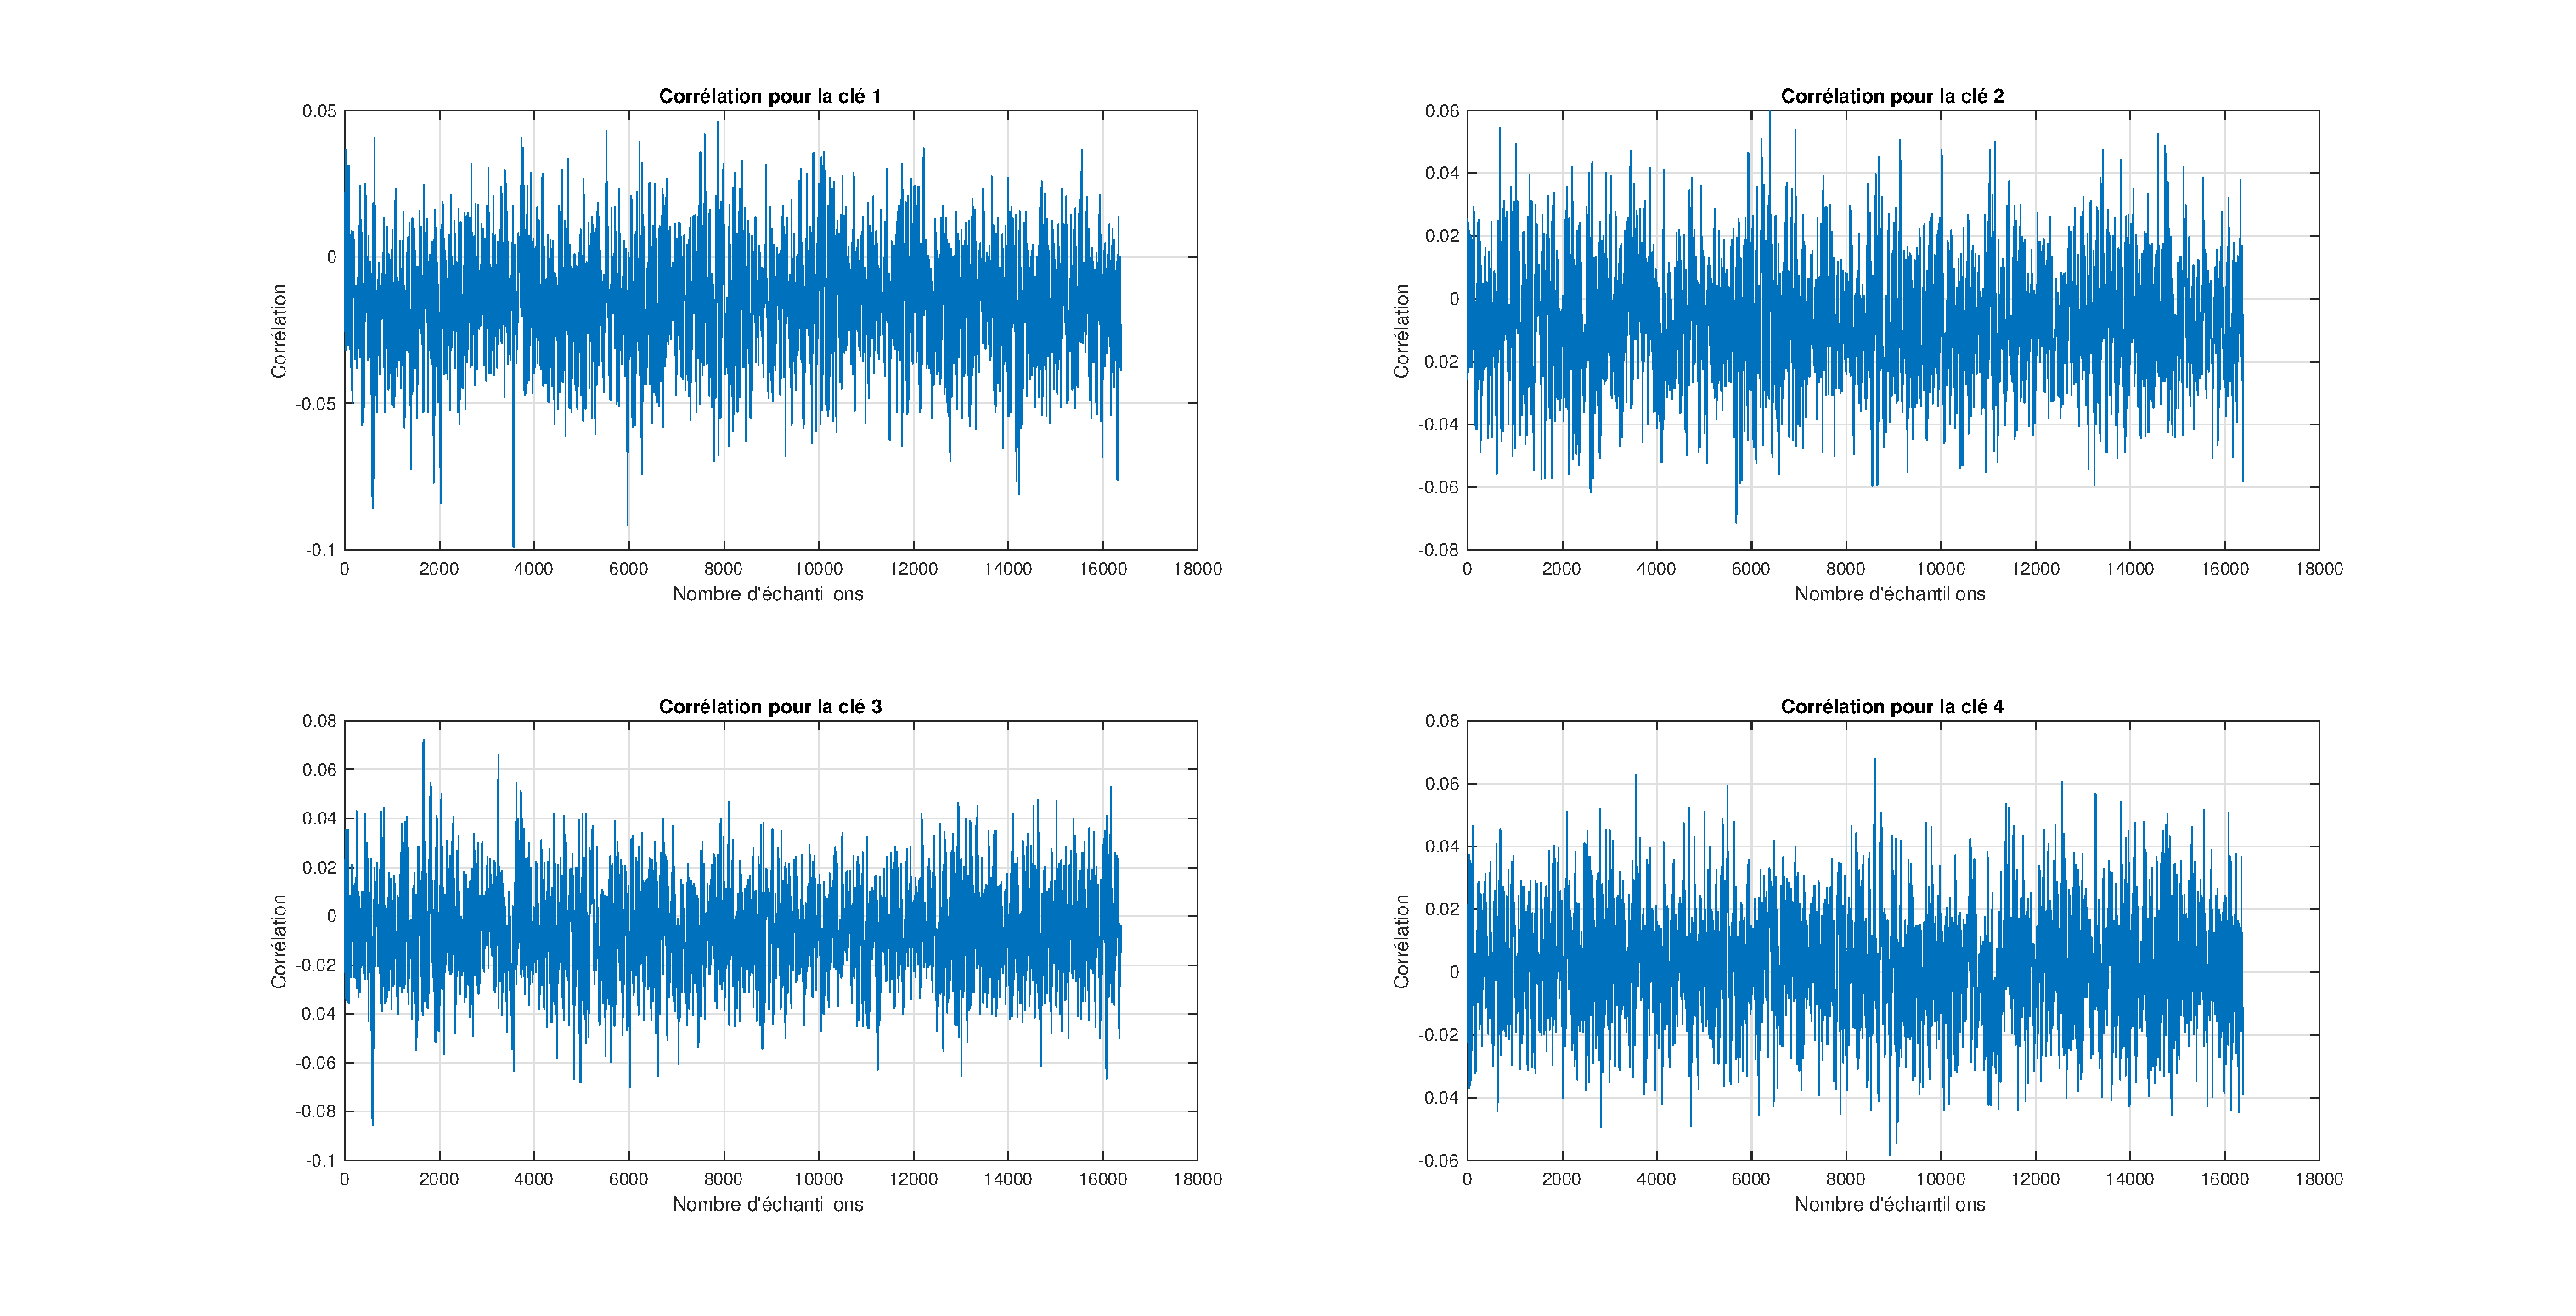
\includegraphics[scale=0.56, angle=90]{image/cle}
    \caption{Les valeurs de coefficient de corrélation obtenues pour les valeurs de clé : 128, 129, 130 et 131 respectivement.}
    \label{fig:cle} 
\end{figure}

\begin{figure}[htbp]
    \centering
    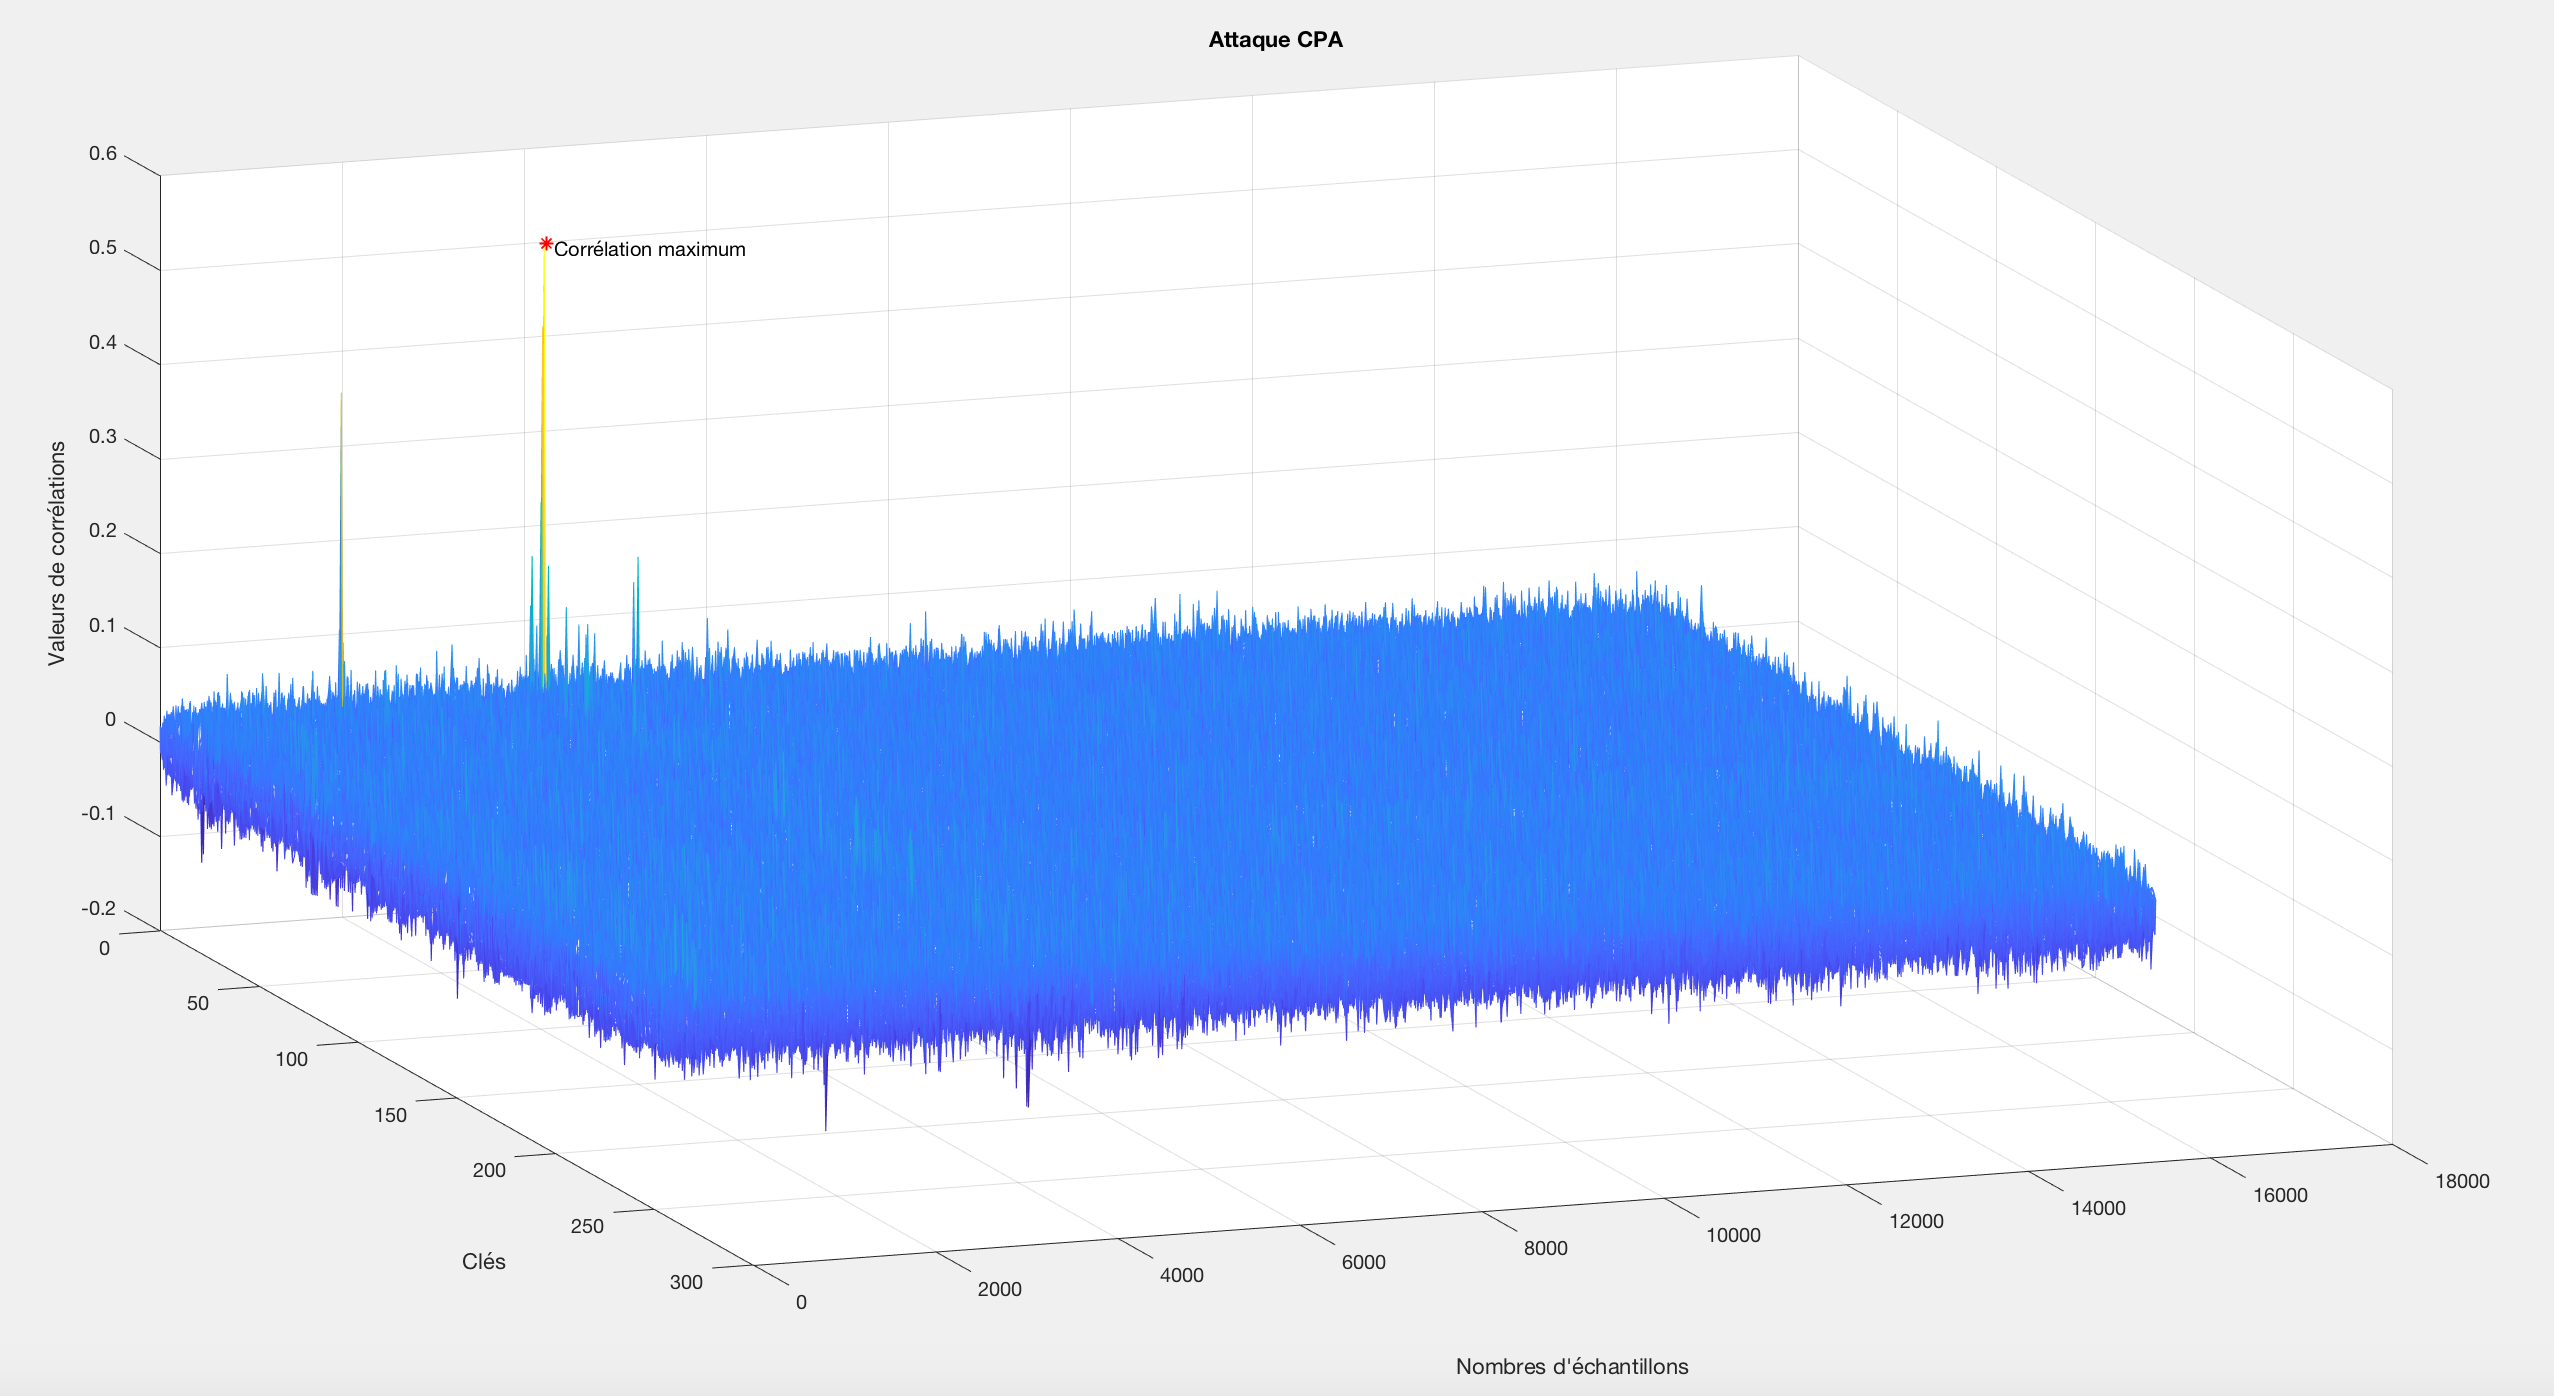
\includegraphics[scale=0.54, angle=90]{image/3D2}
    \caption{Affichage en 3D de toutes les valeurs de corrélation obtenues pour chaque valeur de clé possible.}
    \label{fig:3D} 
\end{figure}

\begin{figure}[htbp]
    \centering
    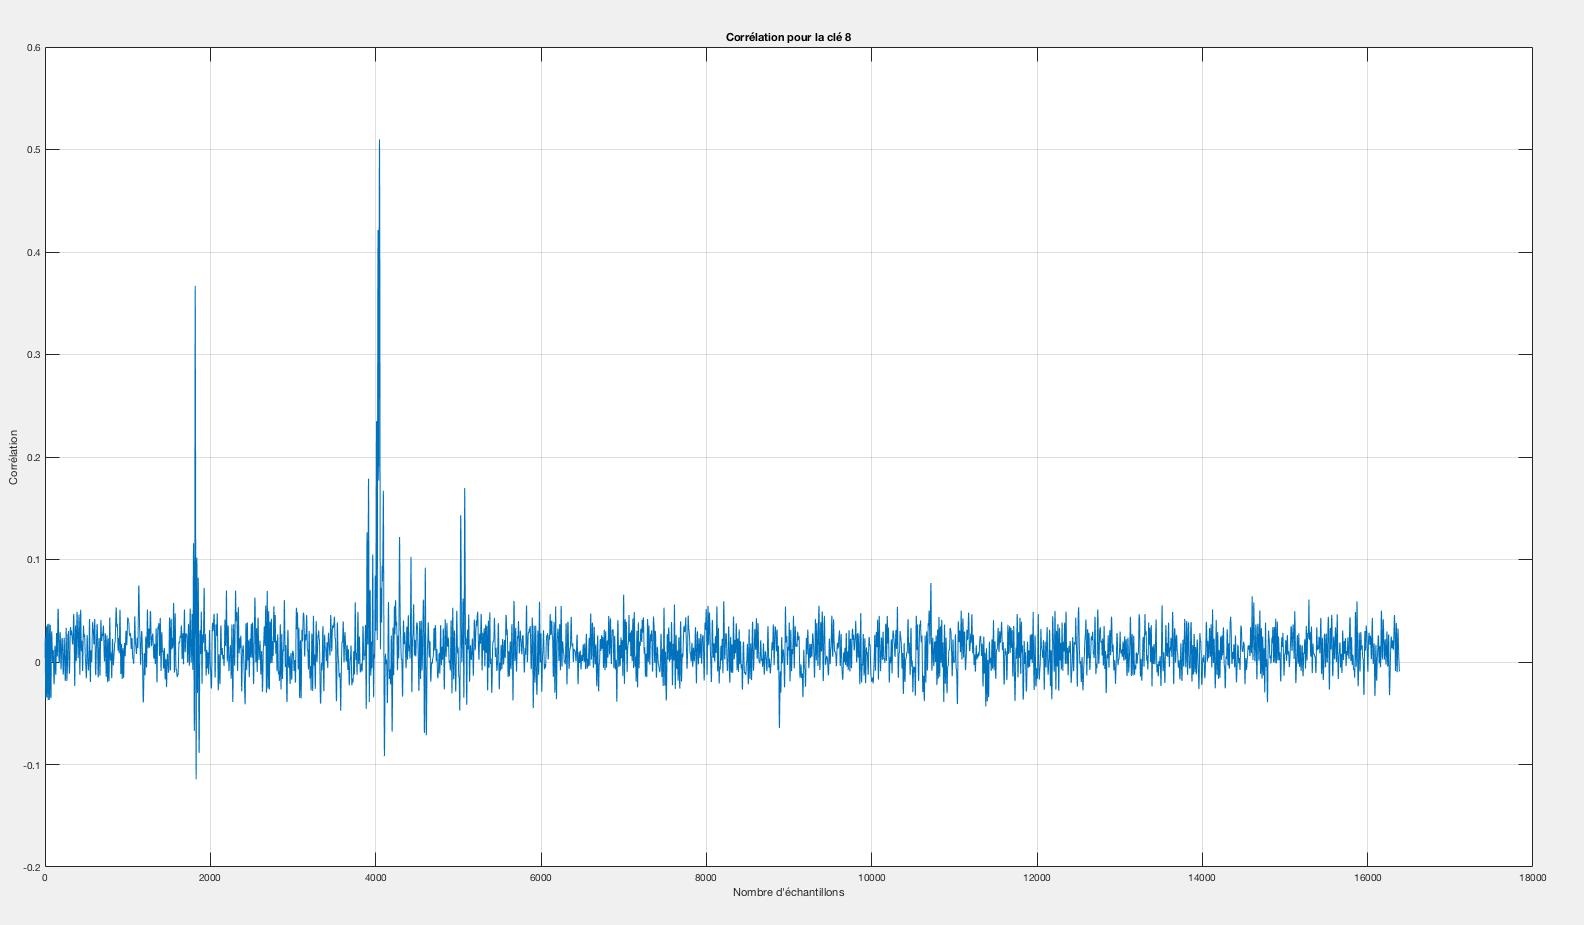
\includegraphics[scale=0.44, angle=90]{image/cle8}
    \caption{Valeurs de corrélation obtenue pour la clé secrète 8 (bonne clé).}
    \label{fig:cle8} 
\end{figure}

\newpage

\subsection{Contre-mesures}
\label{sec:contre-mesures}

\vspace{-0.2 cm}Une fois que les attaques par analyse de la consommation de puissance ont été reconnues comme fonctionnelles, certaines entreprises (comme les banques par exemple) devaient trouver des moyens de contrer ces attaques afin d'assurer la confidentialité des données sensibles qu'elles manipulaient. Par conséquent, une série de contre-mesures a été développée à partir du début du deuxième millénaire. Cette section a pour objectif de présenter ces contre-mesures. 

Pour rappel, les attaques par analyse de la consommation de puissance étudient des traces dont l'allure dépend essentiellement de deux facteurs : les opérations exécutées et les données manipulées. Pour protéger un appareil cryptographique de telles attaques, il faut donc casser les relations entre la consommation de puissance et les données sensibles manipulées et entre la consommation de puissance et les opérations exécutées. Les contre-mesures existantes sont divisées en deux catégories différentes : 
\begin{enumerate}
\item \textbf{Les contre-mesures de type \textit{Hiding}} : Le principe des contre-mesures de type Hiding est de rendre la consommation de puissance du device cryptographique indépendante des opérations exécutées et des données manipulées. Pour ce faire, on verra (section \ref{sec:hiding}) qu'il existe deux approches différentes possibles.
\item \textbf{Les contre-mesures de type \textit{Masking}} : Le principe des contre-mesures de type Masking est de générer des valeurs intermédiaires aléatoires. Ainsi, on accepte que la consommation de puissance du device cryptographique dépende des données manipulées. Cependant, on modifie (on masque) ces valeurs intermédiaires afin que les traces de puissance obtenues à l'oscilloscope soient faussées. On va donc construire des devices cryptographique dont la consommation de puissance est liée aux données manipulées mais ces données sont faussées (modifiées) volontairement. \\
\end{enumerate}

\vspace{-0.2 cm}Il faut noter que les traces de puissance sont en pratique vulgairement caractérisées par des traces en tension. Ainsi, sur un graphe, une trace de puissance est représentée par une courbe indiquant la tension mesurée en fonction du temps. Les contre-mesures développées pour les attaques par analyse de la consommation de puissance ont donc pour objectif de modifier l'allure de ces traces de puissances afin de compliquer la tâche de l'attaquant. Il existe deux façons de modifier une trace de puissance : 
\begin{itemize}
\item \textbf{En agissant sur \textit{l'amplitude} de la trace}, on parlera \textbf{\textit{d'intensité du leakage.}}
\item \textbf{En agissant sur \textit{la position dans le temps} de la trace}, on parlera \textbf{\textit{d'instant du leakage.}} \\
\end{itemize}

\vspace{-0.2 cm}Avant de détailler chacune des deux catégories de contre-mesures, rappelons la définition de rapport signal à bruit (SNR : \textit{Signal to Noise Ratio} en anglais). Le rapport signal à bruit ou SNR est un indicateur de performance. Plus précisément, son objectif est de mesurer la qualité de la transmission d'une information. Sa formulation mathématique est reprise à l'équation (\ref{eqn:SNR}). Elle peut également être exprimée en \textit{dB} (\ref{eqn:SNRdb}) : \\

\begin{minipage}{6cm}
\begin{equation}SNR = \frac{P_{signal}}{P_{noise}} \label{eqn:SNR} \end{equation} 
\end{minipage}
\begin{minipage}{6cm}
\begin{equation}SNR_{dB} = 10.log_{10}\frac{P_{signal}}{P_{noise}} \label{eqn:SNRdb}\end{equation}
\end{minipage}

\hspace{-0.5 cm}Où :
\begin{itemize}
\item $SNR$ représente l'indicateur de performance de la transmission de l'information (sans unité/dB).
\item $P_{signal}$ représente la puissance du signal (en \textit{Watt}).
\item $P_{noise}$ représente la puissance du bruit (en \textit{Watt}). \\
\end{itemize}

\vspace{-0.2 cm}Ainsi, le calcul du SNR permet de savoir si le signal de transmission que l'on étudie est fortement bruité ou non. Selon l'équation (\ref{eqn:SNR}), cet indicateur SNR est d'autant plus élevé que la puissance du signal est élevée ou est d'autant plus élevé que la puissance du bruit est faible. Dans une transmission idéale, on désirera toujours un SNR très grand, signifiant que la trace obtenue représente majoritairement le signal et minoritairment le bruit. \\
Pour une trace de puissance, si le SNR d'une opération est élevé, cela signifie que la puissance du signal est plus élevée que la puissance du bruit, c'est-à-dire qu'il est plus facile de détecter des fuites d'information. Idéalement, il faut donc que le SNR soit proche de 0. De cette façon, le bruit recouvre tellement le signal qu'il est impossible de détecter du leakage. En pratique, cela peut être réalisé en diminuant la variance du signal vers 0 ou en augmentant la variance du bruit vers l'infini.
\begin{itemize}
\item Pour réduire la variance du signal, la consommation de puissance a besoin d'être exactement égale pour toutes les opérations exécutées et données manipulées. En pratique, cela se traduira par de petites valeurs de variances pour le signal.
\item Pour augmenter la variance du bruit, l'amplitude du bruit a besoin d'être augmentée de façon significative laissant croire à l'attaquant l'existence de commutations sur les cellules du device. En pratique, cela se traduira par de grandes valeurs de variances pour le bruit.
\end{itemize}

\newpage

\subsubsection{Contre-mesures \textit{Hiding}}
\label{sec:hiding}
\vspace{-0.1 cm}Comme précisé ci-avant, le principe des contre-mesures de type Hiding est de rendre la consommation de puissance du device cryptographique indépendante des opérations exécutées et des données manipulées. De cette façon, deux approches sont possibles :
\begin{enumerate}
\item Faire en sorte que la consommation de puissance du device cryptographique soit \textbf{\textit{aléatoire}}. Cela signifie qu'à chaque coup de clock, une certaine quantité aléatoire de puissance est consommée. Le but est donc de \textbf{modifier l'instant du leakage} ou bien de \textbf{modifier l'intensité du leakage} dans la trace de puissance.
\begin{itemize}
\item \textit{La modification de l'instant du leakage peut être réalisée par un désalignement des traces}. Cela va compliquer la tâche de l'attaquant. En effet, celui-ci doit, dans un premier temps, procéder à l'alignement de ses traces pour pouvoir les analyser correctement. Si celles-ci ne sont pas alignées, il ne pourra rien en tirer de concret. Ce désalignement des traces peut s’obtenir de différentes façons : utiliser des horloges de fréquences différentes, utiliser des interruptions aléatoires lors de l’exécution du programme, changer l’ordre des instructions, etc.
\item \textit{La modification de l'intensité du leakage peut être réalisée par une modification du rapport signal à bruit}. Nous avons vu que pour modifier le SNR, il suffisait d'augmenter le bruit ou de diminuer le signal. Dans ce cas-ci, nous allons augmenter la variance du bruit. En effet, en ajoutant du bruit de façon indépendante à l'exécution de l'algorithme, on va diminuer le SNR, ce qui va avoir pour conséquence de diminuer le leakage d'une opération : L'attaquant aura dès lors plus de mal à retrouver la clé secrète. 
\end{itemize}
\item Faire en sorte que la consommation de puissance du device cryptographique soit \textbf{\textit{identique}}. Cela signifie qu'à chaque coup de clock, une quantité égale de puissance est consommée pour toutes les opérations exécutées et pour toutes les données manipulées. Le but est donc de \textbf{modifier l'intensité du leakage}. Autrement dit, on souhaite uniformiser l'amplitude de la trace. 
\textit{Pour ce faire, on va à nouveau modifier le rapport signal à bruit}. Comme dit précédemment, l'idéal serait d'avoir un SNR proche de 0. Si on n'augmente pas la variance du bruit, la deuxième approche consiste à diminuer la variance du signal. 
\end{enumerate}

La figure \ref{fig:hiding} ci-dessous présente les mesures possibles selon l'approche suivie tandis que la figure \ref{fig:resume_hiding} page suivante reprend l'ensemble des contre-mesures de type hiding.

\begin{figure}[htbp]
    \centering
    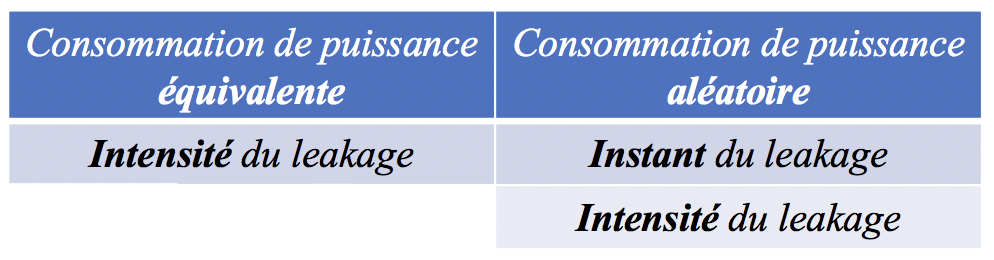
\includegraphics[scale=0.5]{image/hiding}
    \caption{Les contre-mesures de type hiding sont utilisées pour rendre aléatoire ou égale la consommation de puissance du device cryptographique.}
    \label{fig:hiding} 
\end{figure}

\begin{figure}[htbp]
    \centering
    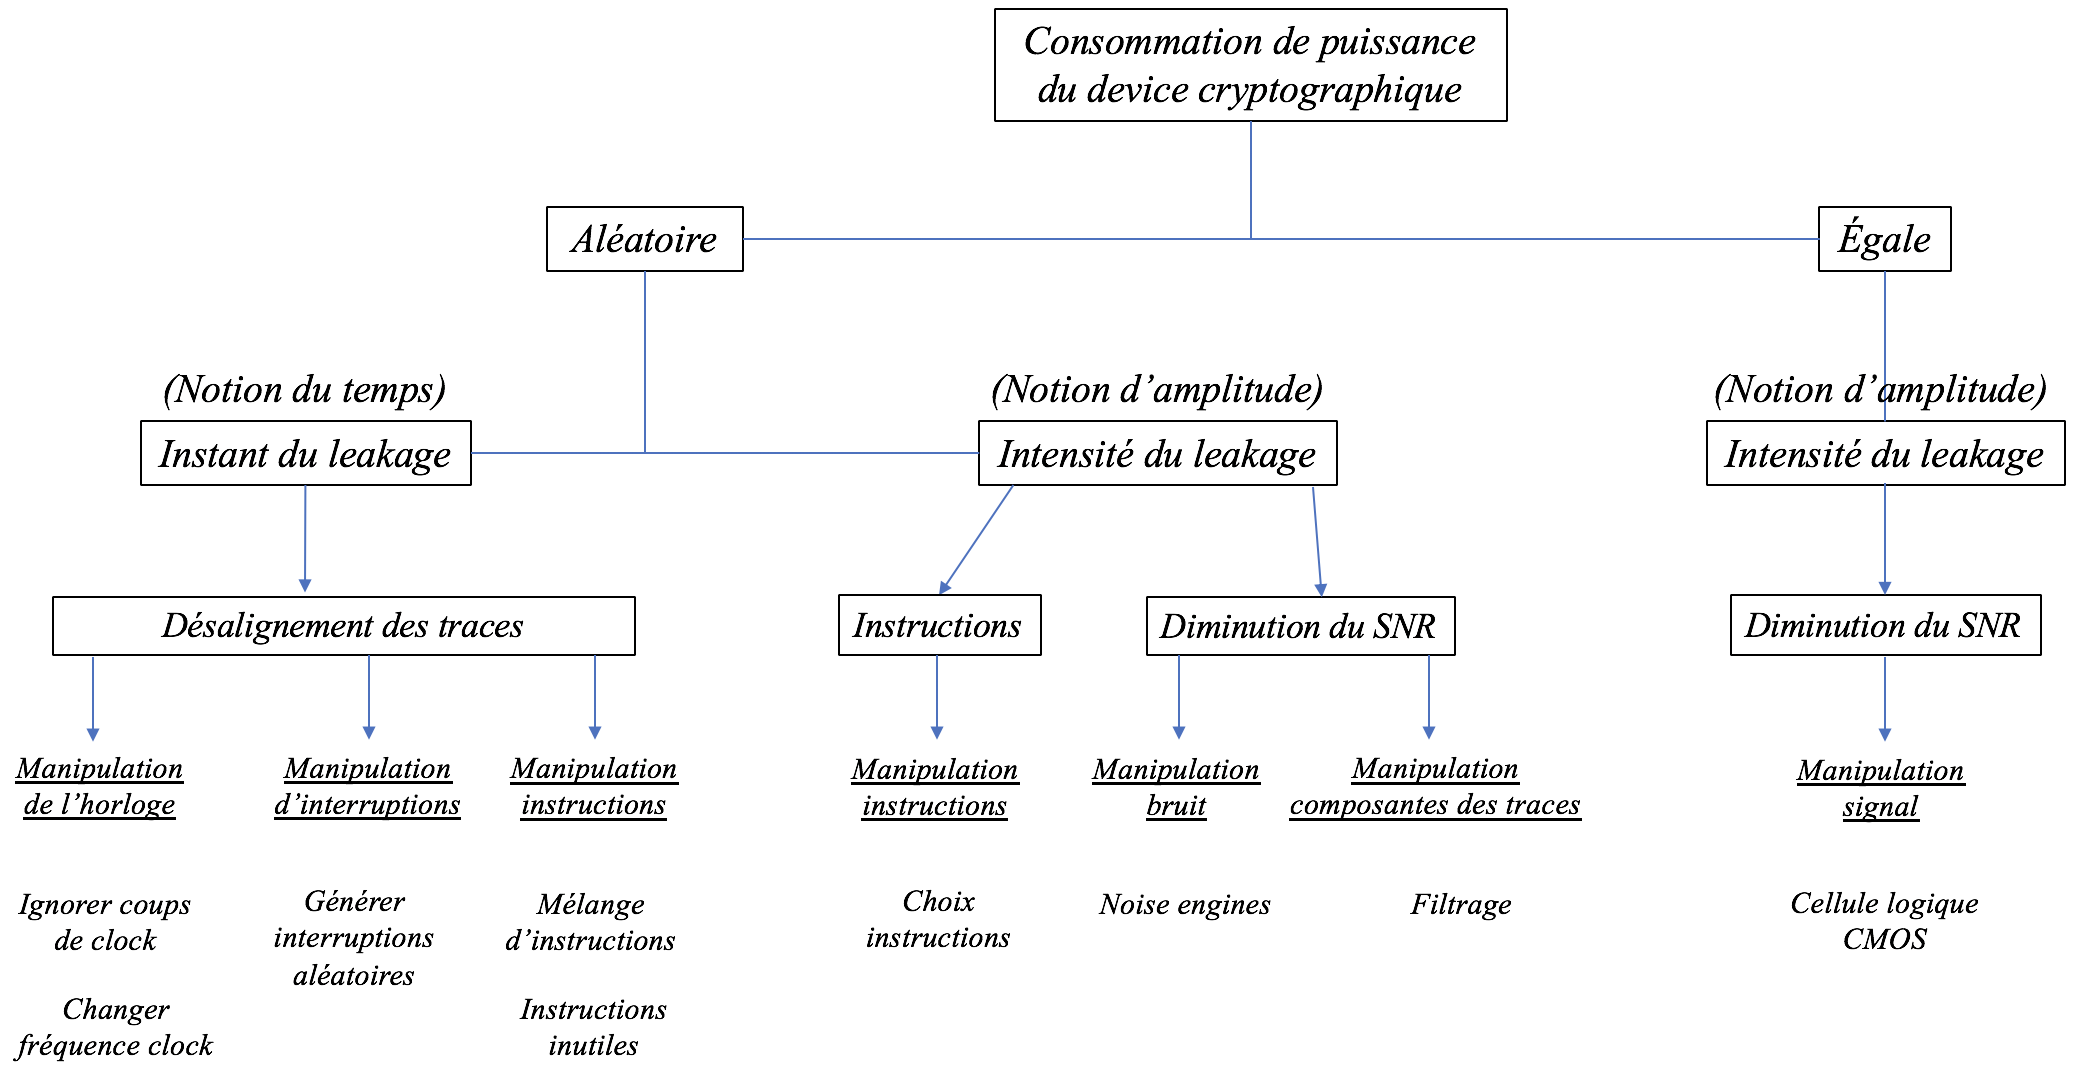
\includegraphics[scale=0.66, angle=90]{image/resume_hiding}
    \caption{Ce schéma présente une partie des contre-mesures de types hiding possibles.}
    \label{fig:resume_hiding} 
\end{figure}

\vspace{-0.4 cm}\hspace{-0.5 cm}Sur base de la figure \ref{fig:resume_hiding}, nous pouvons expliquer le principe de certains exemples de contre-mesures :
\begin{itemize}
\item Concernant la manipulation d’horloge, nous pouvons :
\begin{itemize}
\item Ignorer certains coups de clock : ce qui aura pour effet de retarder l’exécution du prochain cycle, ce qui engendrera donc un désaligenemnt des traces.
\item Changer aléatoirement la fréquence de clock : À l’aide d’un oscillateur et de nombres aléatoires, la fréquence d’horloge est changée à intervalles fréquents, provoquant des vitesses d’exécution différentes et par conséquent un désalignement des traces.
\end{itemize}
\item Concernant les interruptions : on va générer aléatoirement certaines interruptions lors de l'exécution de l'algorithme, ce qui va \textit{casser} (couper) les traces provoquant ainsi un désalignement.
\item Concernant la manipulation d'instructions : 
\begin{itemize}
\item Le mélange des instructions : on va mélanger l’ordre des opérations (seuls les opérations qui peuvent être déplacées ou interverties). Ainsi, pour AES par exemple, il est possible de réaliser l’opération de subBytes sur les 16 bytes de la matrice, dans n’importe quel ordre, sans nuire au déroulement de l’algorithme.
\item Les instructions inutiles : en insérant des opérations inutiles, on va injecter des quantités d'informations inutiles dans chaque trace. Cela provoquera un désalignement des traces.
\item Le choix des instructions : toutes les instructions ne fuitent pas la même quantité d’information sur les opérandes. Il pourrait être bon de choisir les instructions qui révèlent le moins d’informations utiles à un attaquant ou de remplacer certaines instructions par d’autres instructions équivalentes pour que la fuite d’information ne soit pas toujours la même.
\end{itemize}
\item Concernant la diminution du SNR :
\begin{itemize}
\item On peut diminuer le SNR en augmentant la variance du bruit à l'aide de \textit{noise engines}. Il s'agit de composants hardware qui travaillent en parallèle à l’exécution cryptographique. Autrement dit, ces composants hardware vont générer du bruit, ce qui va avoir pour conséquence de diminuer le SNR. En effet, la consommation mesurée sera la somme de la consommation de l’exécution de l’algorithme cryptographique et des composants hardware.
\item On peut diminuer le SNR en diminuant la variance du signal. En pratique, il existe deux possibilités pour diminuer la variance du signal :
\begin{itemize}
\item Une première approche pourrait concerner la cellule logique CMOS en elle-même. On sait (section \ref{sec:puissance}) que la consommation de puissance totale d'un device cryptographique est la somme des puissances consommées par chaque cellule. Ainsi, si chaque cellule consomme une puissance constante, la puissance totale est constante. Il faut donc construire des cellules qui consomment des quantités de puissance constantes.
\item Une seconde approche plus complexe pourrait concerner du filtrage. Il s'agit de filtrer la puissance consommée par le device cryptographique. Le but est alors de supprimer, via ce filtre, toutes les composantes de la trace de puissance qui dépendent des données manipulées et des opérations exécutées. 
\end{itemize}
\end{itemize}
\end{itemize}







\subsubsection{Contre-mesures \textit{Masking}}
Le principe des contre-mesures de type masking est de générer des valeurs intermédiaires aléatoires. Autrement dit, lors de l'exécution d'un algorithme, différentes opérations sont exécutées conduisant à différentes valeurs intermédiaires calculées. Si aucune protection n'est mise en place, la consommation de puissance du device cryptographique dépendra des données intermédiaires qui sont manipulées par le device cryptographique (par l'algorithme pour être plus précis). L'attaquant peut alors potentiellement retrouver la clé secrète en analysant la consommation de puissance du device cryptographique. Par contre, si chaque valeur intermédiaire est dissimulée sous une nouvelle valeur intermédiaire aléatoire dite \textbf{masquée}, alors l'attaquant pourra toujours analyser la consommation de puissance, les traces qu'il obtiendra fourniront des informations faussées (par le masque). En d'autres mots, ce type de contre-mesure accepte que la consommation de puissance du device cryptographique dépendante des données manipulées et des opérations exécutées. Cependant, on va modifier les valeurs intermédiaires de façon aléatoire pour que les traces mesurées à l'oscilloscope n'aient plus de sens. Un avantage de cette approche est qu'elle peut être implémentée au niveau de l'algorithme, c'est-à-dire sans changer les caractéristiques de consommation de puissance du device cryptographique (ce qui est plus complexe) comme c'est le cas pour le contre-mesures Hiding.


\underline{Définition du masque}

Une valeur intermédiaire masquée $v_m$ est une valeur intermédiaire $v$ cachée par une valeur aléatoire $m$ : $v_m = v * m$. Ne connaissant pas la valeur aléatoire $m$, l'attaquant ne peut pas retrouver la valeur intermédiaire $v$. Ainsi, la consommation de puissance du device cryptographique dépend des valeurs intermédiaires masquées $v_m$ qui ne fournissent aucune information sur les valeurs intermédiaires $v$. Autrement dit, un masque cache les valeurs intermédiaires et il n'est donc plus possible de retrouver la clé de chiffrement. Bien évidemment, les masques ont besoin d'être supprimés à la fin des opérations algorithmiques afin d'obtenir le message chiffré. \\
L'opération $*$ représente les opérations exécutées par l'algorithme de chiffrement. Il peut s'agir d'une fonction booléenne ou d'une fonction arithmétique. Ainsi, on définit : 
\begin{enumerate}
\item \textbf{\textit{Un masque booléen}} : l'opération $*$ est alors remplacée par la fonction booléenne XOR (\oplus). Dans ce cas, le masque devient : $v_m = v \oplus m$.
\item \textbf{\textit{Un masque arithmétique}} : l'opération $*$ est alors remplacée par une addition modulaire ($+$) ou par une multiplication modulaire (\times ). Dans ce cas, le masque devient : $v_m = v + m$ $(mod$ $n)$ ou $v_m = v \times m$ $(mod$ $n)$ où \textit{modulo n} est définit en fonction de l'algorithme de chiffrement.
\end{enumerate}

\newpage

\underline{Fonctions linéaires et non-linéaires}

Les algorithmes de chiffrement utilisent des fonctions linéaires mais aussi des fonctions non-linéaires. \textbf{Une fonction est dite \textit{linéaire} si elle respecte la propriété suivante : $f(x*y) = f(x)*f(y)$. À l'inverse, une fonction est dite \textit{non-linéaire} si elle ne respecte pas la propriété}.\\ \\
\textit{Par exemple}, dans l'algorithme AES, on retrouve l'opération XOR. Dans ce cas, l'opération est dite linéaire car la propriété $f(x\oplus m) = f(x) \oplus f(m)$ est respectée. On remarque donc qu'il est facile de calculer un masque booléen pour une fonction linéaire. \\
Un contre-exemple, dans l'algorithme AES, concerne l'opération \textit{SubBytes}. Il s'agit d'une opération non-linéaire. Autrement dit, $f(x\oplus m) \neq f(x) \oplus f(m)$. On remarque donc qu'il n'est pas facile de calculer un masque booléen pour une fonction non-linéaire. Dans ce cas, une alternative est de calculer un masque arithmétique. En effet, la relation $f(x \times m) = (x \times m)^{-1} = f(x) \times f(m)$ est respectée.



\subsubsection{Contre-mesures \textit{Faking}}


\newpage
%%%%%%%%%%%%%%%%%%%%%%%% Partie 4 - Conclusion %%%%%%%%%%%%%%%
\section{Conclusion}


\newpage
%%%%%%%%%%%%%%%%%%%%%%%% CREDITS %%%%%%%%%%%%%%%%%%%%
\pagebreak
\phantomsection
\section*{Crédits}
\addcontentsline{toc}{section}{Crédits}

\begin{itemize}

\item Figure~\ref{fig:thales} provenant du site internet :
\url{http://monipag.com/victoria-petitier/wp-content/uploads/sites/1363/Thales-Group-1.png}

\item Annexe~\ref{ann:Sbox} provenant du site internet de J.M. Dutertre \textit{"Synthèse AES 128"} :
\url{https://www.emse.fr/~dutertre/documents/synth_AES128.pdf}

\end{itemize}

%%%%%%%%%%%%%%%%%%%%%%%% REFERENCES %%%%%%%%%%%%%%%%%%%%

\phantomsection
\addcontentsline{toc}{section}{Références}

\nocite{*}
\bibliography{Stage}
\bibliographystyle{unsrt}


%%%%%%%%%%%%%%%%%%%%%%%% ANNEXES %%%%%%%%%%%%%%%%%%%%
\appendix
\clearpage
\section{Code algorithme AES-128}
\label{ann:AES}
\begin{figure}[!ht]
    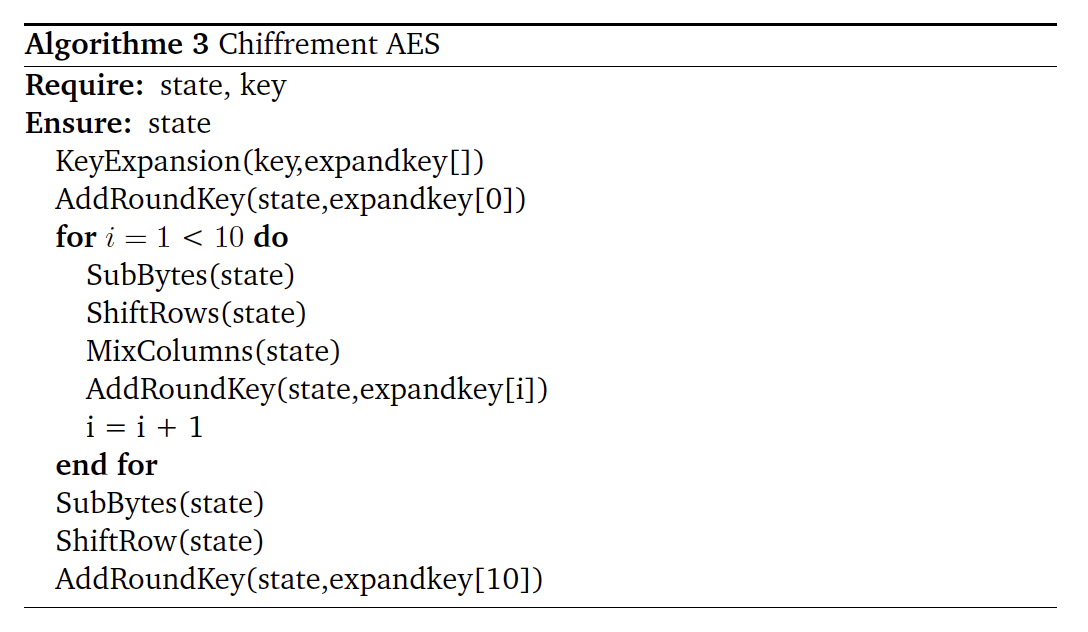
\includegraphics[width=\linewidth]{image/CodeAES}
    \caption{Code définissant l'ordres des opérations exécutées par l'algorithme AES-128.}
    \label{fig:AESCode}
\end{figure}

\section{Sbox - Table de substitution}
\label{ann:Sbox}
\begin{figure}[!ht]
    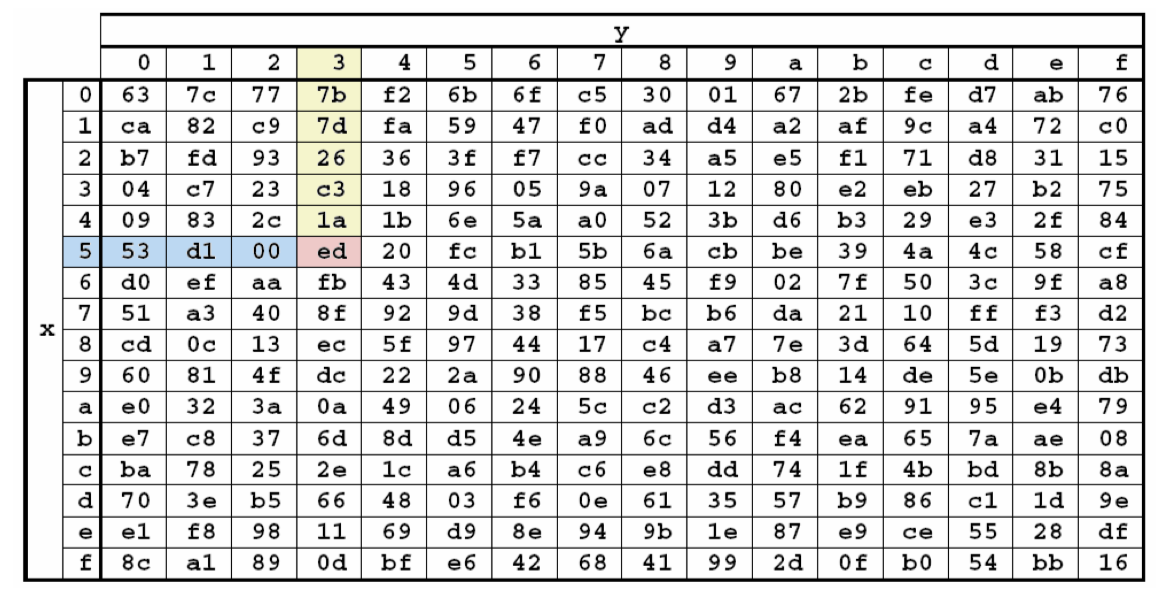
\includegraphics[width=\linewidth]{image/Sbox}
    \caption{La Sbox représente une table de substitution utilisée pour l'opération non-linéaire SubBytes de l'algorithme AES. À chaque donnée hexadécimale d'entrée correspond une donnée hexadécimale de sortie.}
    \label{fig:Sbox}
\end{figure}

\newpage

\section{Opération \textit{KeySchedule}}
\label{ann:KeySchedule}
\begin{figure}[htbp]
    \centering
    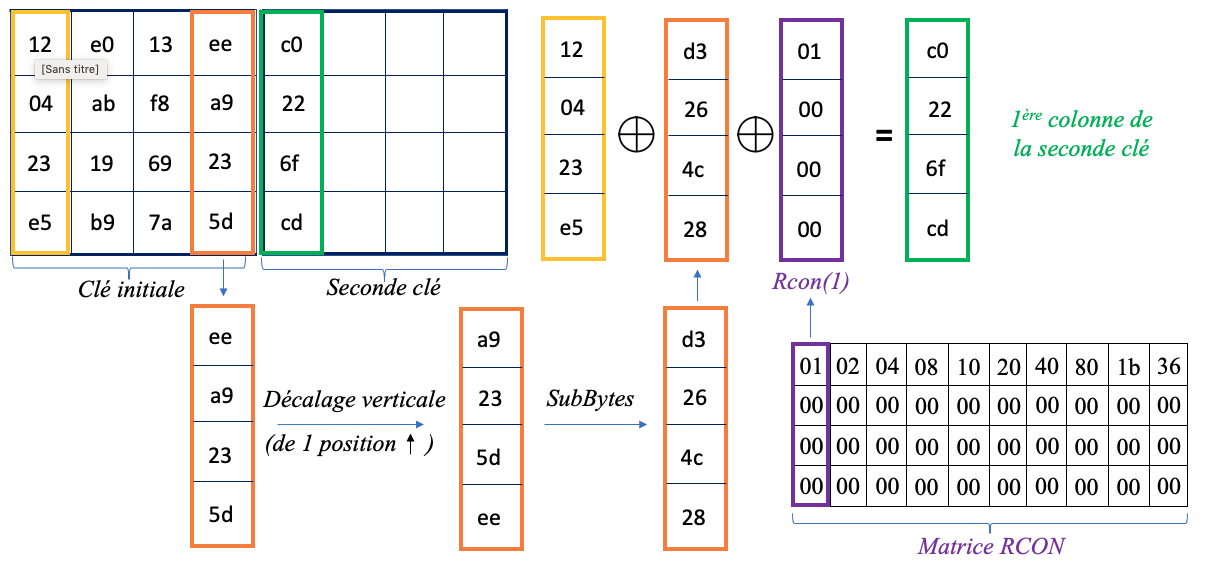
\includegraphics[scale=0.45]{image/KeySchedule1}
     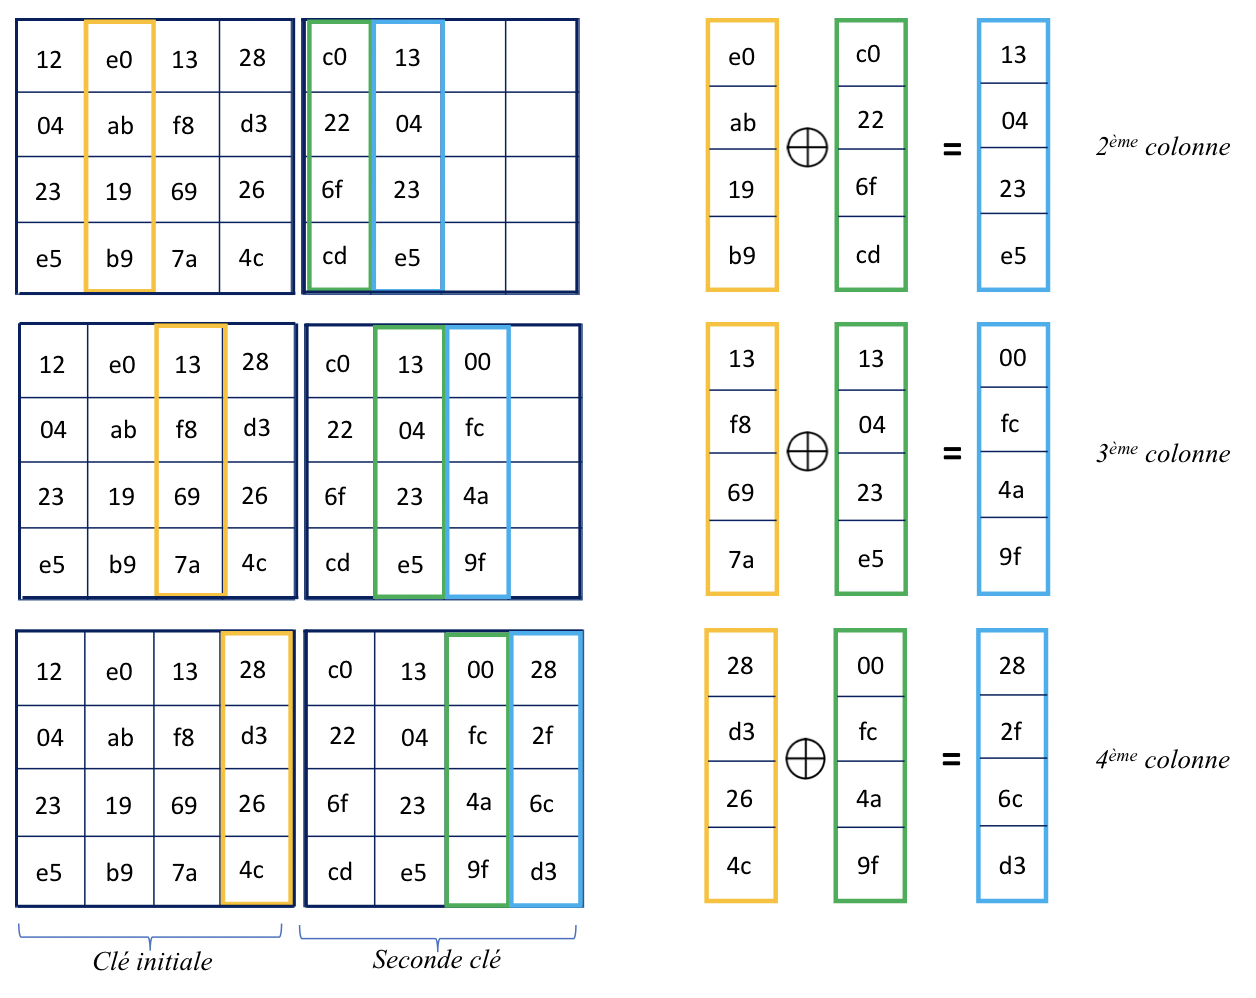
\includegraphics[scale=0.65]{image/KeySchedule2}
    \caption{Principe de fonctionnement de l'opération \textit{KeySchedule}.}
    \label{fig:KeySchedule1}
\end{figure}


\end{document}
